\documentclass[aspectratio=43,10pt]{beamer}
\usepackage[utf8]{inputenc}
\usepackage[vietnamese]{babel}
\usepackage{amsmath,amssymb,amsfonts}
\usepackage{graphicx}
\usepackage{float}
\usepackage{tikz}
\usetikzlibrary{intersections,calc,positioning}
\usepackage{pgfplots}
\pgfplotsset{compat=1.18}

% Thiết lập đường dẫn cho hình ảnh
\makeatletter
\def\input@path{{../}{../figure/}}
% Vô hiệu hóa figure environment cho beamer
\renewenvironment{figure}[1][]{}{}
% Vô hiệu hóa caption cho beamer
\renewcommand{\caption}[1]{}
\renewcommand{\label}[1]{}
\makeatother
\graphicspath{{../figure/}{../}}

\usetheme{Madrid}
\usecolortheme{default}

% Giảm kích thước font cho slide
\setbeamerfont{frametitle}{size=\normalsize}
\setbeamerfont{title}{size=\large}
\setbeamerfont{subtitle}{size=\small}
\setbeamerfont{normal text}{size=\small}

% Sửa footer ngắn gọn
\setbeamertemplate{footline}{
\leavevmode%
\hbox{%
\begin{beamercolorbox}[wd=.5\paperwidth,ht=2.25ex,dp=1ex,center]{author in head/foot}%
\usebeamerfont{author in head/foot}Chuyên đề giải tích số
\end{beamercolorbox}%
\begin{beamercolorbox}[wd=.5\paperwidth,ht=2.25ex,dp=1ex,right]{date in head/foot}%
\usebeamerfont{date in head/foot}\insertframenumber{} / \inserttotalframenumber\hspace*{2ex}
\end{beamercolorbox}}%
\vskip0pt%
}

\title{Phương pháp thể tích hữu hạn cho phương trình Euler}
\subtitle{Nghiên cứu và ứng dụng trong bài toán sóng xung kích}
\author{Nông Thanh Toàn, Nguyễn Hoàng Tú, Lê Minh Tuấn Kiệt, Đặng Kim Bảng}
\institute{Trường Đại học Khoa học Tự nhiên - ĐHQG TP.HCM}
\date{Thành phố Hồ Chí Minh, 2025}

\begin{document}

\frame{\titlepage}

\begin{frame}{Nội dung trình bày}
\tableofcontents[hideallsubsections]
\end{frame}

\section{Giới thiệu}

\begin{frame}{Bài toán nghiên cứu}
\begin{itemize}
    \item \textbf{Hệ phương trình Euler 1D:}
    \begin{align}
        \frac{\partial \rho}{\partial t} + \frac{\partial (\rho u)}{\partial x} &= 0 \\
        \frac{\partial (\rho u)}{\partial t} + \frac{\partial (\rho u^2 + p)}{\partial x} &= 0 \\
        \frac{\partial E}{\partial t} + \frac{\partial (u(E + p))}{\partial x} &= 0
    \end{align}
    
    \item \textbf{Phương trình trạng thái:} $E = \frac{p}{\gamma - 1} + \frac{1}{2}\rho u^2$, $\gamma = 1.4$
\end{itemize}
\end{frame}

\begin{frame}{Bài toán ống sốc Sod}

Xét một ống dài được chia thành hai phần bằng nhau bởi một màng ngăn, với hai bên màng ngăn được bơm khí với mật độ và áp suất khác nhau:
$$
\rho_L = 1.0, \quad \rho_R = 0.125, \quad p_L = 1.0, \quad p_R = 0.1.
$$
và vận tốc ban đầu ở cả hai bên màng ngăn đều bằng 0.

\begin{center}
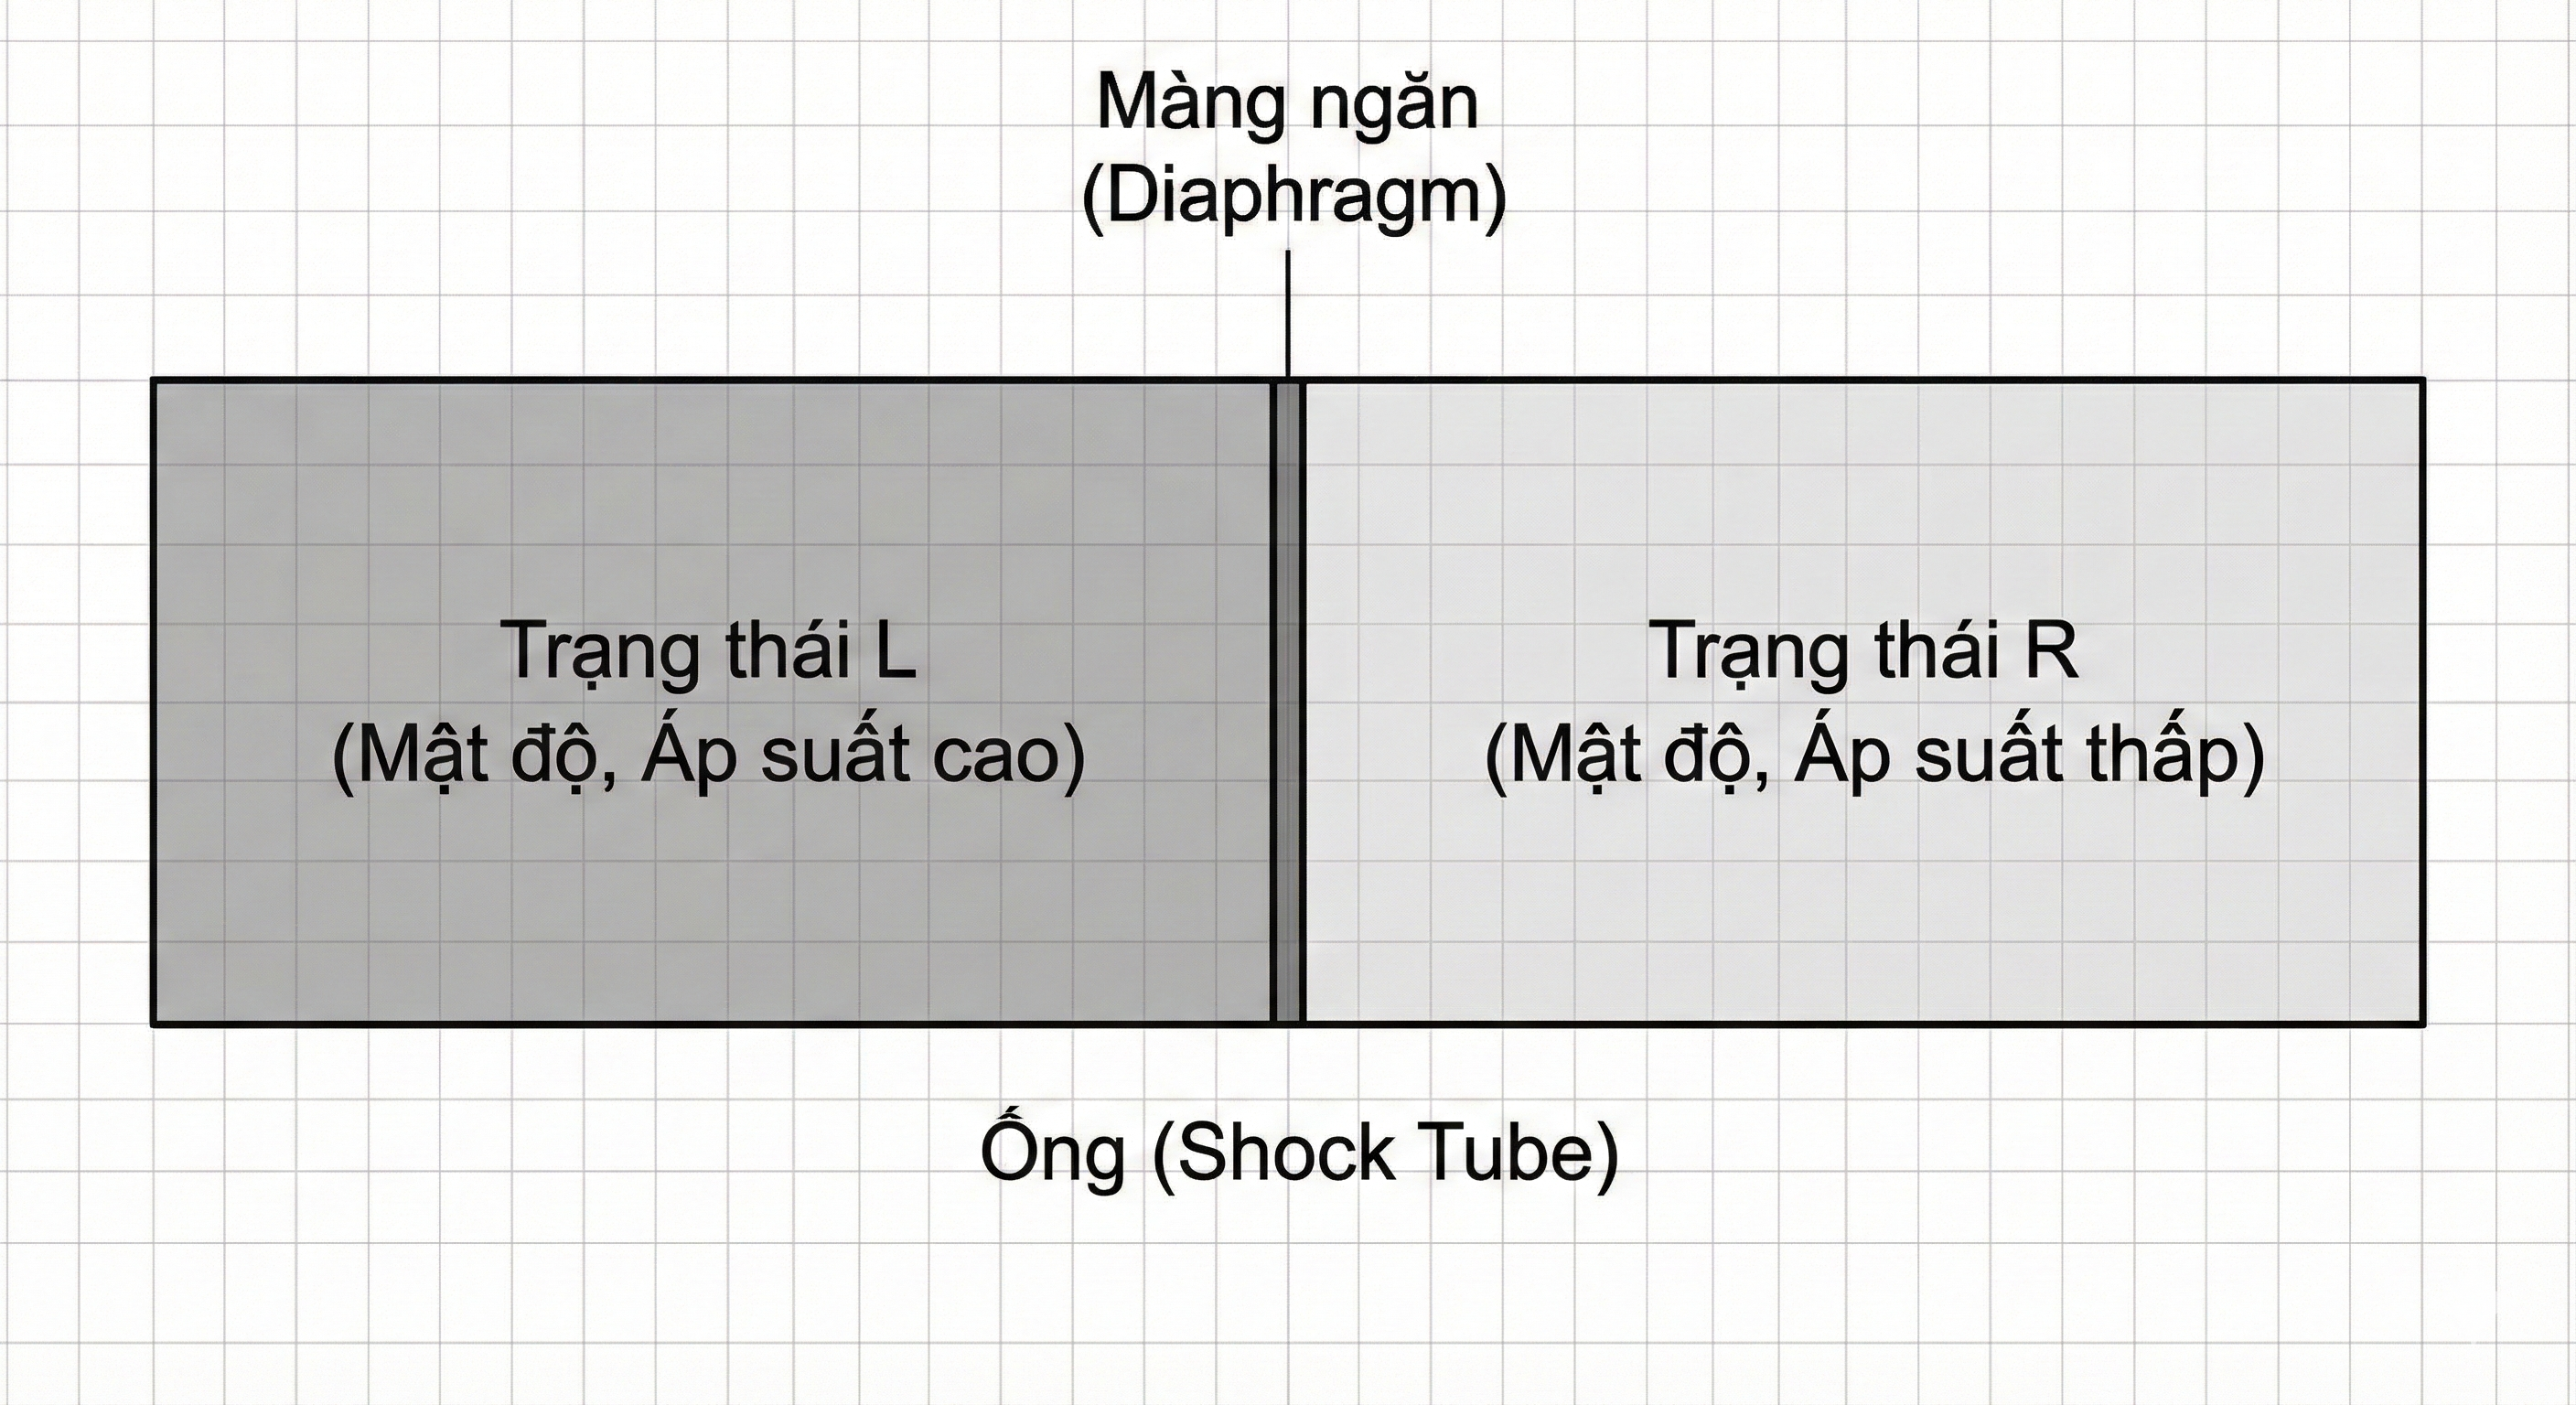
\includegraphics[width=0.5\textwidth]{tube.png}
\end{center}

Khi ta loại bỏ màng ngăn ở thời điểm $t = 0$, thì sẽ có sự biến đổi mật độ, áp suất và vận tốc tại các vị trí trong ống. Mục tiêu của ta là theo dỗi sự biến đổi này.

\end{frame}

\section{Nghiệm chính xác bài toán Riemann}

\begin{frame}{Cấu trúc nghiệm bài toán Riemann}

Giả sử rằng $p_L > p_R$, khi đó cấu trúc nghiệm của bài toán sẽ bao gồm: một sóng giãn (Rarefaction wave) lan truyền về phía trái, một gián đoạn tiếp xúc (Contact discontinuity) ở giữa, và một sóng xung kích (Shock wave) lan truyền về phía phải. Cấu trúc này chia mặt phẳng $x-t$ thành 4 vùng cơ bản: vùng trái ($L$), vùng sao trái ($L^*$), vùng sao phải ($R^*$), và vùng phải ($R$)

\begin{center}
\begin{figure}[H]
\centering
\begin{tikzpicture}[scale=1.5]
    % Draw axes
    \draw[->] (-3,0) -- (3,0) node[right] {$x$};
    \draw[->] (0,0) -- (0,3) node[above] {$t$};
    
    % Origin label
    \node[below] at (0,0) {$x_0$};
    
    % Rarefaction Fan (Left)
    \draw (0,0) -- (-2,2.5) node[above] {Head};
    \draw (0,0) -- (-1,2.5) node[above] {Tail};
    \foreach \i in {-1.8, -1.6, ..., -1.2}
        \draw[dotted] (0,0) -- (\i, 2.5);
        
    % Contact Discontinuity (Middle)
    \draw[dashed, thick] (0,0) -- (0.5,2.5) node[above] {Contact};
    
    % Shock Wave (Right)
    \draw[thick] (0,0) -- (2,2.5) node[above] {Shock};
    
    % Labels for regions
    \node at (-2.5, 1) {$L$};
    \node at (-0.5, 1.8) {$L^*$};
    \node at (1, 1.5) {$R^*$};
    \node at (2.5, 1) {$R$};
    
    % Arrow indicating expansion fan
    \draw[->] (-1.9, 1.2) to[bend left] (-1.1, 1.2);
    \node[below] at (-1.5, 1.2) {Rarefaction};

\end{tikzpicture}
\caption{Cấu trúc nghiệm bài toán Riemann trong mặt phẳng $x-t$ với $p_L > p_R$}
\label{fig:riemann_structure}
\end{figure}
\end{center}
\end{frame}

\begin{frame}{Thuật toán giải nghiệm chính xác}
\textbf{Mục tiêu:} Tìm áp suất vùng sao $p^*$ sao cho $u_L^* = u_R^* = u^*$

\textbf{Bước 1:} Thiết lập các hàm vận tốc
\begin{itemize}
    \item Sóng giãn: $u_L^*(p) = u_L + \frac{2a_L}{\gamma-1}\left[ 1 - \left( \frac{p}{p_L} \right)^{\frac{\gamma-1}{2\gamma}} \right]$
    \item Sóng shock: $u_R^*(p) = u_R + (p - p_R) \sqrt{\frac{A_R}{p + B_R}}$
\end{itemize}

\textbf{Bước 2:} Giải phương trình $f(p) = u_L^*(p) - u_R^*(p) = 0$

\textbf{Bước 3:} Tính các biến trạng thái vùng sao

\textbf{Bước 4:} Xác định nghiệm tại $(x,t)$
\end{frame}

\begin{frame}{Chi tiết Newton-Raphson}
\textbf{Công thức lặp:}
$$p_{k+1} = p_k - \frac{f(p_k)}{f'(p_k)}$$

\textbf{Giá trị khởi tạo:}
$$p_0 = \frac{p_L + p_R}{2}$$

\textbf{Điều kiện dừng:}
$$\frac{|p_{k+1} - p_k|}{p_k} < 10^{-6}$$

\textbf{Hằng số:} $A_R = \frac{2}{(\gamma+1)\rho_R}$, $B_R = \frac{\gamma-1}{\gamma+1}p_R$
\end{frame}

\section{Phương pháp thể tích hữu hạn}

\begin{frame}{Nguyên lý phương pháp thể tích hữu hạn}
Ta có dạng tổng quát của phương trình Euler cho trường hợp một chiều:
\[
w_t + f(w)_x = 0.
\]
Ta xét hệ phương trình trên trên một miền tính toán là $\Omega = \{(x, t) : 0 \leq t \leq t_{\text{final}}, a(t) \leq x \leq b(t) \}$, với $t_{\text{final}}$ là thời điểm cuối cùng mà ta muốn khảo sát, $a(t)$, $b(t)$ là biên của miền tính toán, thỏa điều kiện đầu $u(x, 0) = u_0(x)$.
Ta chia miền $\Omega$ ban đầu thành các miền nhỏ hơn: $[x_{i - 1/2}, x_{i + 1/2}] \times [t^n, t^{n+1}]$.
    
\begin{center}
\begin{figure}[H]
\centering
\begin{tikzpicture}[scale=0.6]
    % Draw axes
    \draw[->] (0,0) -- (6,0) node[right] {$x$};
    \draw[->] (0,0) -- (0,4) node[above] {$t$};
    
    % Draw the domain cell with solid lines
    \draw[thick] (2,1.5) rectangle (4,2.5);
    
    % Dashed lines from axes to domain cell
    \draw[dashed] (2,0) -- (2,1.5);
    \draw[dashed] (4,0) -- (4,1.5);
    \draw[dashed] (0,1.5) -- (2,1.5);
    \draw[dashed] (0,2.5) -- (2,2.5);
    
    % Tick marks on x-axis
    \draw (2,0) -- (2,-0.1);
    \draw (4,0) -- (4,-0.1);
    
    % Tick marks on t-axis
    \draw (0,1.5) -- (-0.1,1.5);
    \draw (0,2.5) -- (-0.1,2.5);
    
    % x-axis labels
    \node[below] at (2,0) {$x_{i-1/2}$};
    \node[below] at (4,0) {$x_{i+1/2}$};
    
    % t-axis labels
    \node[left] at (0,1.5) {$t^n$};
    \node[left] at (0,2.5) {$t^{n+1}$};
    
    % Arrow pointing to the domain with label outside
    \draw[->] (5,3) -- (3.5,2.2);
    \node[right] at (5,3) {$[x_{i-1/2}, x_{i+1/2}] \times [t^n, t^{n+1}]$};
    
\end{tikzpicture}
% \caption{Rời rạc hóa miền tính toán $\Omega$ thành các miền con}
% \label{fig:domain_discretization}
\end{figure}
    
\end{center}
\end{frame}

\begin{frame}{Biến đổi tích phân và công thức cập nhật}
\textbf{Bước 1:} Lấy tích phân trên miền con
$$\int_{t_n}^{t_{n+1}} \int_{x_{i-1/2}}^{x_{i+1/2}} \left( w_t + f(w)_x \right) dx \, dt = 0$$

\textbf{Bước 2:} Áp dụng định lý Newton-Leibniz
$$\int_{x_{i-1/2}}^{x_{i+1/2}} w(x, t_{n+1}) dx - \int_{x_{i-1/2}}^{x_{i+1/2}} w(x, t_n) dx + \int_{t_n}^{t_{n+1}} [f(w(x_{i+1/2}, t)) - f(w(x_{i-1/2}, t))] dt = 0$$

\textbf{Bước 3:} Định nghĩa giá trị trung bình và thông lượng số
$$W_i^n = \frac{1}{\Delta x}\int_{x_{i-1/2}}^{x_{i+1/2}} w(x, t_n) dx, \quad F_{i+1/2} = \frac{1}{\Delta t}\int_{t_n}^{t_{n+1}} f(w(x_{i+1/2}, t)) dt$$

\textbf{Kết quả:} Công thức cập nhật FVM
$$W_i^{n+1} = W_i^n - \frac{\Delta t}{\Delta x} \left( F_{i+1/2} - F_{i-1/2} \right)$$
\end{frame}

\begin{frame}{Xấp xỉ thông lượng số - Three-point stencil}
Giả sử giá trị của $F^n_{i+1/2}$ chỉ phụ thuộc vào các giá trị của $W_i^n$ và $W_{i+1}^{n}$, khi đó ta có thể xấp xỉ $F^n_{i+1/2}$ như sau:

\[
F^n_{i+1/2} \approx \mathcal{F} (W_i^n, W^n_{i+1}).
\]
Bằng cách xấp xỉ tương tự cho $F^n_{i-1/2}$, ta có kết quả sau:
\[
[W]_i^{n+1} = [W]_i^n - \frac{\Delta t}{\Delta x_i} \left( \mathcal{F} (W_i^n, W^n_{i+1}) - \mathcal{F} (W_{i-1}^n, W^n_{i})\right).
\]

Cách xấp xỉ như trên làm cho $W_i^{n+1}$ chỉ phụ thuộc vào $W_{i-1}^{n}, W_i^{n}$ và $W_{i+1}^{n}$, do đó ta gọi nó là phương pháp three-point stencil. Với mỗi cách chọn $\mathcal{F}$, ta có được một phương pháp số cho phương trình Euler.

Ta chọn $F^n_{i+1/2} \approx \mathcal{F} (W_i^n, W^n_{i+1}) = \dfrac{1}{2}(f(W_i^n) + f(W_{i+1}^n))$, khi đó phương trình cập nhật trở thành:
\begin{align*}
    W_i^{n+1} &=  W_i^n - \frac{\Delta t}{2\Delta x} \left[ f(W_i^n) + f(W_{i+1}^n) - f(W_{i-1}^n) - f(W_i^n) \right] \\ 
    &= W_i^n - \frac{\Delta t}{2\Delta x} \left( f(W_{i+1}^n) - f(W_{i-1}^n)\right) 
\end{align*}


\end{frame}

\begin{frame}{Phương pháp Lax-Friedrichs}
Phương pháp Lax-Friedrich là một trong những phương pháp đơn giản nhất để giải hệ phương trình Euler. Bằng cách thay đổi $W_i^n = \dfrac{W_{i+1}^n + W_{i-1}^n}{2}$ vào phương trình sai phân trung tâm, ta có được phương pháp Lax-Friedrich:
\[
W_i^{n+1} = \dfrac{W_{i-1}^n + W_{i+1}^n}{2} - \frac{\Delta t}{2\Delta x} \left( f(W_{i+1}^n) - f(W_{i-1}^n) \right).
\]
Đặc điểm của phương pháp Lax-Friedrich:
\begin{itemize}
    \small
    \item Sai số lớn tại vùng shock và contact discontinuity
    \item Hiện tượng tán xạ (smearing) rõ rệt
    \item Độ chính xác thấp nhưng ổn định
\end{itemize}
Dưới đây là kết quả áp dụng phương pháp Lax-Friedrich cho bài toán:
\end{frame}

\begin{frame}{Kết quả Lax-Friedrichs}
\begin{center}
\scalebox{0.6}{\begin{figure}[H]
\centering
\begin{tikzpicture}
    % Define spacing and dimensions
    \def\plotwidth{7cm}
    \def\plotheight{5.5cm}
    \def\hspace{8cm}
    \def\vspace{6.5cm}
    
    % Top row
    \node[anchor=south west, fill=white] at (0,\vspace) {
        \resizebox{\plotwidth}{\plotheight}{% This file was created by matlab2tikz.
%
%The latest updates can be retrieved from
%  http://www.mathworks.com/matlabcentral/fileexchange/22022-matlab2tikz-matlab2tikz
%where you can also make suggestions and rate matlab2tikz.
%
\definecolor{mycolor1}{rgb}{0.12941,0.12941,0.12941}%
%
\begin{tikzpicture}

\begin{axis}[%
width=3.229in,
height=2.498in,
at={(0.542in,0.392in)},
scale only axis,
xmin=0,
xmax=1,
xlabel style={font=\color{mycolor1}},
xlabel={x},
ymin=0.1,
ymax=1,
ylabel style={font=\color{mycolor1}},
ylabel={$\text{Density (}\rho\text{)}$},
axis background/.style={fill=white},
title style={font=\bfseries\color{mycolor1}},
title={Lax-Friedrichs Density Distribution},
xmajorgrids,
ymajorgrids,
legend style={legend cell align=left, align=left}
]
\addplot [color=blue, line width=2.0pt]
  table[row sep=crcr]{%
0	0.999998258674086\\
0.0050251256281407	0.999998258674086\\
0.0100502512562814	0.999997158031474\\
0.0150753768844221	0.999997158031474\\
0.0201005025125628	0.999993960385556\\
0.0251256281407035	0.999993960385556\\
0.0301507537688442	0.999987331053824\\
0.0351758793969849	0.999987331053824\\
0.0402010050251256	0.999974306385863\\
0.0452261306532663	0.999974306385863\\
0.050251256281407	0.999949649995506\\
0.0552763819095477	0.999949649995506\\
0.0603015075376884	0.999904600941577\\
0.0653266331658292	0.999904600941577\\
0.0703517587939698	0.999825110253605\\
0.0753768844221105	0.999825110253605\\
0.0804020100502513	0.999689571424351\\
0.085427135678392	0.999689571424351\\
0.0904522613065327	0.999466129261941\\
0.0954773869346734	0.999466129261941\\
0.100502512562814	0.999109792029165\\
0.105527638190955	0.999109792029165\\
0.110552763819095	0.998559738035543\\
0.115577889447236	0.998559738035543\\
0.120603015075377	0.997737356666548\\
0.125628140703518	0.997737356666548\\
0.130653266331658	0.996545638678143\\
0.135678391959799	0.996545638678143\\
0.14070351758794	0.994870475887804\\
0.14572864321608	0.994870475887804\\
0.150753768844221	0.992584215482233\\
0.155778894472362	0.992584215482233\\
0.160804020100503	0.989551455854656\\
0.165829145728643	0.989551455854656\\
0.170854271356784	0.985636641408037\\
0.175879396984925	0.985636641408037\\
0.180904522613065	0.980712624638726\\
0.185929648241206	0.980712624638726\\
0.190954773869347	0.974669128140635\\
0.195979899497487	0.974669128140635\\
0.201005025125628	0.967420028086455\\
0.206030150753769	0.967420028086455\\
0.21105527638191	0.958908595520745\\
0.21608040201005	0.958908595520745\\
0.221105527638191	0.949110205482028\\
0.226130653266332	0.949110205482028\\
0.231155778894472	0.938032450461357\\
0.236180904522613	0.938032450461357\\
0.241206030150754	0.925712969257643\\
0.246231155778894	0.925712969257643\\
0.251256281407035	0.912215554136316\\
0.256281407035176	0.912215554136316\\
0.261306532663317	0.897625204731094\\
0.266331658291457	0.897625204731094\\
0.271356783919598	0.882042773741923\\
0.276381909547739	0.882042773741923\\
0.281407035175879	0.865579738320631\\
0.28643216080402	0.865579738320631\\
0.291457286432161	0.848353478530375\\
0.296482412060302	0.848353478530375\\
0.301507537688442	0.830483289023292\\
0.306532663316583	0.830483289023292\\
0.311557788944724	0.812087217074702\\
0.316582914572864	0.812087217074702\\
0.321608040201005	0.793279720757579\\
0.326633165829146	0.793279720757579\\
0.331658291457286	0.774170076505514\\
0.336683417085427	0.774170076505514\\
0.341708542713568	0.754861430669598\\
0.346733668341709	0.754861430669598\\
0.351758793969849	0.735450377453233\\
0.35678391959799	0.735450377453233\\
0.361809045226131	0.716026948183909\\
0.366834170854271	0.716026948183909\\
0.371859296482412	0.696674907741938\\
0.376884422110553	0.696674907741938\\
0.381909547738693	0.67747226815296\\
0.386934673366834	0.67747226815296\\
0.391959798994975	0.658491943391131\\
0.396984924623116	0.658491943391131\\
0.402010050251256	0.639802481053911\\
0.407035175879397	0.639802481053911\\
0.412060301507538	0.621468814323378\\
0.417085427135678	0.621468814323378\\
0.422110552763819	0.603552980638621\\
0.42713567839196	0.603552980638621\\
0.4321608040201	0.586114751247608\\
0.437185929648241	0.586114751247608\\
0.442211055276382	0.56921210808866\\
0.447236180904523	0.56921210808866\\
0.452261306532663	0.552901491547567\\
0.457286432160804	0.552901491547567\\
0.462311557788945	0.537237725666756\\
0.467336683417085	0.537237725666756\\
0.472361809045226	0.522273508934371\\
0.477386934673367	0.522273508934371\\
0.482412060301508	0.508058343748125\\
0.487437185929648	0.508058343748125\\
0.492462311557789	0.494636774126054\\
0.49748743718593	0.494636774126054\\
0.50251256281407	0.482045821043267\\
0.507537688442211	0.482045821043267\\
0.512562814070352	0.470311562847773\\
0.517587939698492	0.470311562847773\\
0.522613065326633	0.459444919804426\\
0.527638190954774	0.459444919804426\\
0.532663316582915	0.4494368765261\\
0.537688442211055	0.4494368765261\\
0.542713567839196	0.4402536086084\\
0.547738693467337	0.4402536086084\\
0.552763819095477	0.431832239809118\\
0.557788944723618	0.431832239809118\\
0.562814070351759	0.424078182011587\\
0.5678391959799	0.424078182011587\\
0.57286432160804	0.416865114518571\\
0.577889447236181	0.416865114518571\\
0.582914572864322	0.410038550907304\\
0.587939698492462	0.410038550907304\\
0.592964824120603	0.40342356319841\\
0.597989949748744	0.40342356319841\\
0.603015075376884	0.396836598699914\\
0.608040201005025	0.396836598699914\\
0.613065326633166	0.390100539058563\\
0.618090452261307	0.390100539058563\\
0.623115577889447	0.383061390644362\\
0.628140703517588	0.383061390644362\\
0.633165829145729	0.375604456829846\\
0.638190954773869	0.375604456829846\\
0.64321608040201	0.367667676009173\\
0.648241206030151	0.367667676009173\\
0.653266331658292	0.359250069152967\\
0.658291457286432	0.359250069152967\\
0.663316582914573	0.350413875709734\\
0.668341708542714	0.350413875709734\\
0.673366834170854	0.341279834325959\\
0.678391959798995	0.341279834325959\\
0.683417085427136	0.332016016323179\\
0.688442211055276	0.332016016323179\\
0.693467336683417	0.322821481045337\\
0.698492462311558	0.322821481045337\\
0.703517587939699	0.313906658272723\\
0.708542713567839	0.313906658272723\\
0.71356783919598	0.305472675771766\\
0.718592964824121	0.305472675771766\\
0.723618090452261	0.297691776496801\\
0.728643216080402	0.297691776496801\\
0.733668341708543	0.290690479155551\\
0.738693467336683	0.290690479155551\\
0.743718592964824	0.284536229357029\\
0.748743718592965	0.284536229357029\\
0.753768844221106	0.279227002181657\\
0.758793969849246	0.279227002181657\\
0.763819095477387	0.274681730293125\\
0.768844221105528	0.274681730293125\\
0.773869346733668	0.270727718442816\\
0.778894472361809	0.270727718442816\\
0.78391959798995	0.267079824438749\\
0.78894472361809	0.267079824438749\\
0.793969849246231	0.263306442201109\\
0.798994974874372	0.263306442201109\\
0.804020100502513	0.258782667092942\\
0.809045226130653	0.258782667092942\\
0.814070351758794	0.252649132000028\\
0.819095477386935	0.252649132000028\\
0.824120603015075	0.243837521263082\\
0.829145728643216	0.243837521263082\\
0.834170854271357	0.23128983941941\\
0.839195979899497	0.23128983941941\\
0.844221105527638	0.214515904876155\\
0.849246231155779	0.214515904876155\\
0.85427135678392	0.19439651193949\\
0.85929648241206	0.19439651193949\\
0.864321608040201	0.173548335473074\\
0.869346733668342	0.173548335473074\\
0.874371859296482	0.155354259314585\\
0.879396984924623	0.155354259314585\\
0.884422110552764	0.142055548427925\\
0.889447236180904	0.142055548427925\\
0.894472361809045	0.133771801376835\\
0.899497487437186	0.133771801376835\\
0.904522613065327	0.129224902756225\\
0.909547738693467	0.129224902756225\\
0.914572864321608	0.126943118672822\\
0.919597989949749	0.126943118672822\\
0.924623115577889	0.125864436203158\\
0.92964824120603	0.125864436203158\\
0.934673366834171	0.125374576407908\\
0.939698492462312	0.125374576407908\\
0.944723618090452	0.125158561602955\\
0.949748743718593	0.125158561602955\\
0.954773869346734	0.125065609579864\\
0.959798994974874	0.125065609579864\\
0.964824120603015	0.125026521322311\\
0.969849246231156	0.125026521322311\\
0.974874371859296	0.125010471494743\\
0.979899497487437	0.125010471494743\\
0.984924623115578	0.125004117809962\\
0.989949748743719	0.125004117809962\\
0.994974874371859	0.125002237860314\\
1	0.125002237860314\\
};
\addlegendentry{LF Solution}

\end{axis}
\end{tikzpicture}%}
    };
    
    \node[anchor=south west, fill=white] at (\hspace,\vspace) {
        \resizebox{\plotwidth}{\plotheight}{% This file was created by matlab2tikz.
%
%The latest updates can be retrieved from
%  http://www.mathworks.com/matlabcentral/fileexchange/22022-matlab2tikz-matlab2tikz
%where you can also make suggestions and rate matlab2tikz.
%
\definecolor{mycolor1}{rgb}{0.12941,0.12941,0.12941}%
%
\begin{tikzpicture}

\begin{axis}[%
width=3.229in,
height=2.498in,
at={(0.542in,0.392in)},
scale only axis,
xmin=0,
xmax=1,
xlabel style={font=\color{mycolor1}},
xlabel={x},
ymin=0,
ymax=1,
ylabel style={font=\color{mycolor1}},
ylabel={Velocity (u)},
axis background/.style={fill=white},
title style={font=\bfseries\color{mycolor1}},
title={Lax-Friedrichs Velocity Distribution},
xmajorgrids,
ymajorgrids,
legend style={legend cell align=left, align=left}
]
\addplot [color=red, line width=2.0pt]
  table[row sep=crcr]{%
0	2.06036324041918e-06\\
0.0050251256281407	2.06036324041918e-06\\
0.0100502512562814	3.36265861710774e-06\\
0.0150753768844221	3.36265861710774e-06\\
0.0201005025125628	7.14615245128612e-06\\
0.0251256281407035	7.14615245128612e-06\\
0.0301507537688442	1.49900430316176e-05\\
0.0351758793969849	1.49900430316176e-05\\
0.0402010050251256	3.04009126164035e-05\\
0.0452261306532663	3.04009126164035e-05\\
0.050251256281407	5.95744020942169e-05\\
0.0552763819095477	5.95744020942169e-05\\
0.0603015075376884	0.000112876346982274\\
0.0653266331658292	0.000112876346982274\\
0.0703517587939698	0.000206929492666156\\
0.0753768844221105	0.000206929492666156\\
0.0804020100502513	0.00036729980550932\\
0.085427135678392	0.00036729980550932\\
0.0904522613065327	0.000631684506043909\\
0.0954773869346734	0.000631684506043909\\
0.100502512562814	0.0010533406115355\\
0.105527638190955	0.0010533406115355\\
0.110552763819095	0.00170430169408887\\
0.115577889447236	0.00170430169408887\\
0.120603015075377	0.00267776348169563\\
0.125628140703518	0.00267776348169563\\
0.130653266331658	0.0040889420678909\\
0.135678391959799	0.0040889420678909\\
0.14070351758794	0.00607378414520779\\
0.14572864321608	0.00607378414520779\\
0.150753768844221	0.00878516643709386\\
0.155778894472362	0.00878516643709386\\
0.160804020100503	0.012386633240322\\
0.165829145728643	0.012386633240322\\
0.170854271356784	0.0170441958187177\\
0.175879396984925	0.0170441958187177\\
0.180904522613065	0.0229171259793809\\
0.185929648241206	0.0229171259793809\\
0.190954773869347	0.0301488978468447\\
0.195979899497487	0.0301488978468447\\
0.201005025125628	0.0388594026909874\\
0.206030150753769	0.0388594026909874\\
0.21105527638191	0.0491392987149729\\
0.21608040201005	0.0491392987149729\\
0.221105527638191	0.061046947689434\\
0.226130653266332	0.061046947689434\\
0.231155778894472	0.0746079510032226\\
0.236180904522613	0.0746079510032226\\
0.241206030150754	0.0898169335359206\\
0.246231155778894	0.0898169335359206\\
0.251256281407035	0.106640996031596\\
0.256281407035176	0.106640996031596\\
0.261306532663317	0.125024176695531\\
0.266331658291457	0.125024176695531\\
0.271356783919598	0.144892303814866\\
0.276381909547739	0.144892303814866\\
0.281407035175879	0.16615773836621\\
0.28643216080402	0.16615773836621\\
0.291457286432161	0.188723653543851\\
0.296482412060302	0.188723653543851\\
0.301507537688442	0.212487642212414\\
0.306532663316583	0.212487642212414\\
0.311557788944724	0.23734456283668\\
0.316582914572864	0.23734456283668\\
0.321608040201005	0.263188621392526\\
0.326633165829146	0.263188621392526\\
0.331658291457286	0.289914741780604\\
0.336683417085427	0.289914741780604\\
0.341708542713568	0.317419305777712\\
0.346733668341709	0.317419305777712\\
0.351758793969849	0.345600352689511\\
0.35678391959799	0.345600352689511\\
0.361809045226131	0.374357325522354\\
0.366834170854271	0.374357325522354\\
0.371859296482412	0.403590440478316\\
0.376884422110553	0.403590440478316\\
0.381909547738693	0.433199744397591\\
0.386934673366834	0.433199744397591\\
0.391959798994975	0.463083913811193\\
0.396984924623116	0.463083913811193\\
0.402010050251256	0.493138842149891\\
0.407035175879397	0.493138842149891\\
0.412060301507538	0.523256060631971\\
0.417085427135678	0.523256060631971\\
0.422110552763819	0.553321045611355\\
0.42713567839196	0.553321045611355\\
0.4321608040201	0.583211483006845\\
0.437185929648241	0.583211483006845\\
0.442211055276382	0.612795591187413\\
0.447236180904523	0.612795591187413\\
0.452261306532663	0.641930649267859\\
0.457286432160804	0.641930649267859\\
0.462311557788945	0.670461938612832\\
0.467336683417085	0.670461938612832\\
0.472361809045226	0.698222378575923\\
0.477386934673367	0.698222378575923\\
0.482412060301508	0.725033214173659\\
0.487437185929648	0.725033214173659\\
0.492462311557789	0.750706175171193\\
0.49748743718593	0.750706175171193\\
0.50251256281407	0.775047542408226\\
0.507537688442211	0.775047542408226\\
0.512562814070352	0.797864485629091\\
0.517587939698492	0.797864485629091\\
0.522613065326633	0.818973830208117\\
0.527638190954774	0.818973830208117\\
0.532663316582915	0.838213033475923\\
0.537688442211055	0.838213033475923\\
0.542713567839196	0.855452612225189\\
0.547738693467337	0.855452612225189\\
0.552763819095477	0.870608642655314\\
0.557788944723618	0.870608642655314\\
0.562814070351759	0.883653422502688\\
0.5678391959799	0.883653422502688\\
0.57286432160804	0.894622172394238\\
0.577889447236181	0.894622172394238\\
0.582914572864322	0.903613963632275\\
0.587939698492462	0.903613963632275\\
0.592964824120603	0.910785951841079\\
0.597989949748744	0.910785951841079\\
0.603015075376884	0.916341299503918\\
0.608040201005025	0.916341299503918\\
0.613065326633166	0.920512507653032\\
0.618090452261307	0.920512507653032\\
0.623115577889447	0.923542810537015\\
0.628140703517588	0.923542810537015\\
0.633165829145729	0.925668519424172\\
0.638190954773869	0.925668519424172\\
0.64321608040201	0.927104706127573\\
0.648241206030151	0.927104706127573\\
0.653266331658292	0.928035624273504\\
0.658291457286432	0.928035624273504\\
0.663316582914573	0.928610130715194\\
0.668341708542714	0.928610130715194\\
0.673366834170854	0.928941405250657\\
0.678391959798995	0.928941405250657\\
0.683417085427136	0.929109644715483\\
0.688442211055276	0.929109644715483\\
0.693467336683417	0.929166135978696\\
0.698492462311558	0.929166135978696\\
0.703517587939699	0.929137076640309\\
0.708542713567839	0.929137076640309\\
0.71356783919598	0.92902552716445\\
0.718592964824121	0.92902552716445\\
0.723618090452261	0.928809723491327\\
0.728643216080402	0.928809723491327\\
0.733668341708543	0.928435408298736\\
0.738693467336683	0.928435408298736\\
0.743718592964824	0.927798568433855\\
0.748743718592965	0.927798568433855\\
0.753768844221106	0.926712662535625\\
0.758793969849246	0.926712662535625\\
0.763819095477387	0.924850730793864\\
0.768844221105528	0.924850730793864\\
0.773869346733668	0.92164749765667\\
0.778894472361809	0.92164749765667\\
0.78391959798995	0.916140304151359\\
0.78894472361809	0.916140304151359\\
0.793969849246231	0.90672374526868\\
0.798994974874372	0.90672374526868\\
0.804020100502513	0.890802226908472\\
0.809045226130653	0.890802226908472\\
0.814070351758794	0.86437667993431\\
0.819095477386935	0.86437667993431\\
0.824120603015075	0.821759332524212\\
0.829145728643216	0.821759332524212\\
0.834170854271357	0.755961278742321\\
0.839195979899497	0.755961278742321\\
0.844221105527638	0.660804026508322\\
0.849246231155779	0.660804026508322\\
0.85427135678392	0.535792503536017\\
0.85929648241206	0.535792503536017\\
0.864321608040201	0.392343481928518\\
0.869346733668342	0.392343481928518\\
0.874371859296482	0.254309597865968\\
0.879396984924623	0.254309597865968\\
0.884422110552764	0.14571647010679\\
0.889447236180904	0.14571647010679\\
0.894472361809045	0.0753236230090875\\
0.899497487437186	0.0753236230090875\\
0.904522613065327	0.0361935796887442\\
0.909547738693467	0.0361935796887442\\
0.914572864321608	0.0165788812706796\\
0.919597989949749	0.0165788812706796\\
0.924623115577889	0.0073513466857154\\
0.92964824120603	0.0073513466857154\\
0.934673366834171	0.00317884511561765\\
0.939698492462312	0.00317884511561765\\
0.944723618090452	0.00134405423122103\\
0.949748743718593	0.00134405423122103\\
0.954773869346734	0.000555800041100139\\
0.959798994974874	0.000555800041100139\\
0.964824120603015	0.000224601651482036\\
0.969849246231156	0.000224601651482036\\
0.974874371859296	8.86670037435969e-05\\
0.979899497487437	8.86670037435969e-05\\
0.984924623115578	3.48649556972697e-05\\
0.989949748743719	3.48649556972697e-05\\
0.994974874371859	1.89471868760348e-05\\
1	1.89471868760348e-05\\
};
\addlegendentry{LF Solution}

\end{axis}
\end{tikzpicture}%}
    };
    
    % Bottom row
    \node[anchor=south west, fill=white] at (0,0) {
        \resizebox{\plotwidth}{\plotheight}{% This file was created by matlab2tikz.
%
%The latest updates can be retrieved from
%  http://www.mathworks.com/matlabcentral/fileexchange/22022-matlab2tikz-matlab2tikz
%where you can also make suggestions and rate matlab2tikz.
%
\definecolor{mycolor1}{rgb}{0.12941,0.12941,0.12941}%
%
\begin{tikzpicture}

\begin{axis}[%
width=3.229in,
height=2.498in,
at={(0.542in,0.392in)},
scale only axis,
xmin=0,
xmax=1,
xlabel style={font=\color{mycolor1}},
xlabel={x},
ymin=0.1,
ymax=1,
ylabel style={font=\color{mycolor1}},
ylabel={Pressure (p)},
axis background/.style={fill=white},
title style={font=\bfseries\color{mycolor1}},
title={Lax-Friedrichs Pressure Distribution},
xmajorgrids,
ymajorgrids,
legend style={legend cell align=left, align=left}
]
\addplot [color=green, line width=2.0pt]
  table[row sep=crcr]{%
0	0.999997562147529\\
0.0050251256281407	0.999997562147529\\
0.0100502512562814	0.999996021254339\\
0.0150753768844221	0.999996021254339\\
0.0201005025125628	0.999991544583892\\
0.0251256281407035	0.999991544583892\\
0.0301507537688442	0.9999822636553\\
0.0351758793969849	0.9999822636553\\
0.0402010050251256	0.999964029627012\\
0.0452261306532663	0.999964029627012\\
0.050251256281407	0.999929512449228\\
0.0552763819095477	0.999929512449228\\
0.0603015075376884	0.999866449552029\\
0.0653266331658292	0.999866449552029\\
0.0703517587939698	0.999755180279986\\
0.0753768844221105	0.999755180279986\\
0.0804020100502513	0.999565476732363\\
0.085427135678392	0.999565476732363\\
0.0904522613065327	0.999252794773278\\
0.0954773869346734	0.999252794773278\\
0.100502512562814	0.998754270286759\\
0.105527638190955	0.998754270286759\\
0.110552763819095	0.997985024715732\\
0.115577889447236	0.997985024715732\\
0.120603015075377	0.9968355589178\\
0.125628140703518	0.9968355589178\\
0.130653266331658	0.995171123208581\\
0.135678391959799	0.995171123208581\\
0.14070351758794	0.992833871780376\\
0.14572864321608	0.992833871780376\\
0.150753768844221	0.989648293992091\\
0.155778894472362	0.989648293992091\\
0.160804020100503	0.985429885267673\\
0.165829145728643	0.985429885267673\\
0.170854271356784	0.979996381866661\\
0.175879396984925	0.979996381866661\\
0.180904522613065	0.973180303438463\\
0.185929648241206	0.973180303438463\\
0.190954773869347	0.964841197356966\\
0.195979899497487	0.964841197356966\\
0.201005025125628	0.954875970021523\\
0.206030150753769	0.954875970021523\\
0.21105527638191	0.943226026603689\\
0.21608040201005	0.943226026603689\\
0.221105527638191	0.929880519789545\\
0.226130653266332	0.929880519789545\\
0.231155778894472	0.914875665375506\\
0.236180904522613	0.914875665375506\\
0.241206030150754	0.89829065481281\\
0.246231155778894	0.89829065481281\\
0.251256281407035	0.880241071899891\\
0.256281407035176	0.880241071899891\\
0.261306532663317	0.860870867364795\\
0.266331658291457	0.860870867364795\\
0.271356783919598	0.840343890577654\\
0.276381909547739	0.840343890577654\\
0.281407035175879	0.818835788865236\\
0.28643216080402	0.818835788865236\\
0.291457286432161	0.796526836226483\\
0.296482412060302	0.796526836226483\\
0.301507537688442	0.77359600566993\\
0.306532663316583	0.77359600566993\\
0.311557788944724	0.750216391499326\\
0.316582914572864	0.750216391499326\\
0.321608040201005	0.726551936335834\\
0.326633165829146	0.726551936335834\\
0.331658291457286	0.702755322878266\\
0.336683417085427	0.702755322878266\\
0.341708542713568	0.678966843357537\\
0.346733668341709	0.678966843357537\\
0.351758793969849	0.655314047692121\\
0.35678391959799	0.655314047692121\\
0.361809045226131	0.631911982023562\\
0.366834170854271	0.631911982023562\\
0.371859296482412	0.608863852254264\\
0.376884422110553	0.608863852254264\\
0.381909547738693	0.586261974802805\\
0.386934673366834	0.586261974802805\\
0.391959798994975	0.564188903964394\\
0.396984924623116	0.564188903964394\\
0.402010050251256	0.542718648967501\\
0.407035175879397	0.542718648967501\\
0.412060301507538	0.521917912429136\\
0.417085427135678	0.521917912429136\\
0.422110552763819	0.501847294717621\\
0.42713567839196	0.501847294717621\\
0.4321608040201	0.482562415561953\\
0.437185929648241	0.482562415561953\\
0.442211055276382	0.464114905275842\\
0.447236180904523	0.464114905275842\\
0.452261306532663	0.446553213697661\\
0.457286432160804	0.446553213697661\\
0.462311557788945	0.429923176396491\\
0.467336683417085	0.429923176396491\\
0.472361809045226	0.414268266742812\\
0.477386934673367	0.414268266742812\\
0.482412060301508	0.399629452372736\\
0.487437185929648	0.399629452372736\\
0.492462311557789	0.386044570631609\\
0.49748743718593	0.386044570631609\\
0.50251256281407	0.373547147287251\\
0.507537688442211	0.373547147287251\\
0.512562814070352	0.362164615499507\\
0.517587939698492	0.362164615499507\\
0.522613065326633	0.351915956957871\\
0.527638190954774	0.351915956957871\\
0.532663316582915	0.342808889347643\\
0.537688442211055	0.342808889347643\\
0.542713567839196	0.334836858806792\\
0.547738693467337	0.334836858806792\\
0.552763819095477	0.327976241296203\\
0.557788944723618	0.327976241296203\\
0.562814070351759	0.322184272358208\\
0.5678391959799	0.322184272358208\\
0.57286432160804	0.317398257426597\\
0.577889447236181	0.317398257426597\\
0.582914572864322	0.313536516891631\\
0.587939698492462	0.313536516891631\\
0.592964824120603	0.31050127504426\\
0.597989949748744	0.31050127504426\\
0.603015075376884	0.308183345880475\\
0.608040201005025	0.308183345880475\\
0.613065326633166	0.306468090593386\\
0.618090452261307	0.306468090593386\\
0.623115577889447	0.305241835514045\\
0.628140703517588	0.305241835514045\\
0.633165829145729	0.304397838031403\\
0.638190954773869	0.304397838031403\\
0.64321608040201	0.303841002508293\\
0.648241206030151	0.303841002508293\\
0.653266331658292	0.303490835330482\\
0.658291457286432	0.303490835330482\\
0.663316582914573	0.303282492261658\\
0.668341708542714	0.303282492261658\\
0.673366834170854	0.30316610409622\\
0.678391959798995	0.30316610409622\\
0.683417085427136	0.303104784727934\\
0.688442211055276	0.303104784727934\\
0.693467336683417	0.303071788982059\\
0.698492462311558	0.303071788982059\\
0.703517587939699	0.303047196260897\\
0.708542713567839	0.303047196260897\\
0.71356783919598	0.303014273299197\\
0.718592964824121	0.303014273299197\\
0.723618090452261	0.302955336635784\\
0.728643216080402	0.302955336635784\\
0.733668341708543	0.302846489759687\\
0.738693467336683	0.302846489759687\\
0.743718592964824	0.302650008548988\\
0.748743718592965	0.302650008548988\\
0.753768844221106	0.302302310755431\\
0.758793969849246	0.302302310755431\\
0.763819095477387	0.301694291414098\\
0.768844221105528	0.301694291414098\\
0.773869346733668	0.300639394189702\\
0.778894472361809	0.300639394189702\\
0.78391959798995	0.298823704798339\\
0.78894472361809	0.298823704798339\\
0.793969849246231	0.295733717388382\\
0.798994974874372	0.295733717388382\\
0.804020100502513	0.290567092827512\\
0.809045226130653	0.290567092827512\\
0.814070351758794	0.282162510234559\\
0.819095477386935	0.282162510234559\\
0.824120603015075	0.269054740678023\\
0.829145728643216	0.269054740678023\\
0.834170854271357	0.249862883285666\\
0.839195979899497	0.249862883285666\\
0.844221105527638	0.224219418319934\\
0.849246231155779	0.224219418319934\\
0.85427135678392	0.194002456049316\\
0.85929648241206	0.194002456049316\\
0.864321608040201	0.163662688613954\\
0.869346733668342	0.163662688613954\\
0.874371859296482	0.138319589432588\\
0.879396984924623	0.138319589432588\\
0.884422110552764	0.120734310869637\\
0.889447236180904	0.120734310869637\\
0.894472361809045	0.110335928173583\\
0.899497487437186	0.110335928173583\\
0.904522613065327	0.104870291326925\\
0.909547738693467	0.104870291326925\\
0.914572864321608	0.102209883488706\\
0.919597989949749	0.102209883488706\\
0.924623115577889	0.100975690838694\\
0.92964824120603	0.100975690838694\\
0.934673366834171	0.100421107617311\\
0.939698492462312	0.100421107617311\\
0.944723618090452	0.100177904608843\\
0.949748743718593	0.100177904608843\\
0.954773869346734	0.10007354276037\\
0.959798994974874	0.10007354276037\\
0.964824120603015	0.100029714790825\\
0.969849246231156	0.100029714790825\\
0.974874371859296	0.100011729969812\\
0.979899497487437	0.100011729969812\\
0.984924623115578	0.100004612266805\\
0.989949748743719	0.100004612266805\\
0.994974874371859	0.100002506498085\\
1	0.100002506498085\\
};
\addlegendentry{LF Solution}

\end{axis}
\end{tikzpicture}%}
    };
    
\end{tikzpicture}
\caption{Kết quả phương pháp Lax-Friedrichs tại t = 0.2}
\label{fig:lf_results}
\end{figure}}
\end{center}
\vspace{-0.3cm}
\end{frame}

\begin{frame}{Phương pháp Local Lax-Friedrichs}
Phương pháp local Lax-Friedrich (LLF) là phương pháp cải tiến cho Lax-Friedrich. Phương pháp này hoạt động bằng cách thay thế giá trị $\dfrac{\Delta t}{\Delta x}$ bằng một giá trị cục bộ $\alpha$. Thành phần được thêm vào này được gọi là vận tốc truyền sóng cực đại (Maximum Local Wave Speed):
\[
F_{i+1/2}^{LLF}(W_-, W_+) = \frac{1}{2} \left( f(W_-) + f(W_+) \right) - \dfrac{\alpha_{1/2}}{2} \left( W_+ - W_- \right).
\]
Hệ số $\alpha_{i+1/2}$ được tính bằng công thức
\[
\alpha_{i+1/2} = \max \left( |f'(W_i)|, |f'(W_{i+1})| \right)
\]
đối với phương trình vô hướng, còn đối với phương trình Euler thì ta có:
\[
\alpha_{i+1/2} = \max \left( |\lambda(A(W_i))|, |\lambda(A(W_{i+1}))| \right)
\]

Dưới đây là kết quả áp dụng phương pháp Local Lax-Friedrich cho bài toán:
\end{frame}

\begin{frame}{Kết quả Local Lax-Friedrichs}
\begin{center}
\scalebox{0.6}{\begin{tikzpicture}
    % Define spacing and dimensions
    \def\plotwidth{7cm}
    \def\plotheight{5.5cm}
    \def\hspace{8cm}
    \def\vspace{6.5cm}
    
    % Top row
    \node[anchor=south west, fill=white] at (0,\vspace) {
        \resizebox{\plotwidth}{\plotheight}{% This file was created by matlab2tikz.
%
%The latest updates can be retrieved from
%  http://www.mathworks.com/matlabcentral/fileexchange/22022-matlab2tikz-matlab2tikz
%where you can also make suggestions and rate matlab2tikz.
%
\definecolor{mycolor1}{rgb}{0.12941,0.12941,0.12941}%
%
\begin{tikzpicture}

\begin{axis}[%
width=3.229in,
height=2.498in,
at={(0.542in,0.392in)},
scale only axis,
xmin=0,
xmax=1,
xlabel style={font=\color{mycolor1}},
xlabel={x},
ymin=0.1,
ymax=1,
ylabel style={font=\color{mycolor1}},
ylabel={$\text{Density (}\rho\text{)}$},
axis background/.style={fill=white},
title style={font=\bfseries\color{mycolor1}},
title={Local Lax-Friedrichs Density Distribution},
xmajorgrids,
ymajorgrids,
legend style={legend cell align=left, align=left}
]
\addplot [color=blue, line width=2.0pt]
  table[row sep=crcr]{%
0	1\\
0.0050251256281407	1\\
0.0100502512562814	1\\
0.0150753768844221	1\\
0.0201005025125628	0.999999999999999\\
0.0251256281407035	0.999999999999997\\
0.0301507537688442	0.999999999999989\\
0.0351758793969849	0.999999999999964\\
0.0402010050251256	0.999999999999888\\
0.0452261306532663	0.999999999999657\\
0.050251256281407	0.999999999998975\\
0.0552763819095477	0.999999999997004\\
0.0603015075376884	0.999999999991443\\
0.0653266331658292	0.999999999976125\\
0.0703517587939698	0.999999999934928\\
0.0753768844221105	0.999999999826737\\
0.0804020100502513	0.999999999549314\\
0.085427135678392	0.999999998854747\\
0.0904522613065327	0.999999997156958\\
0.0954773869346734	0.999999993105318\\
0.100502512562814	0.999999983666239\\
0.105527638190955	0.999999962200332\\
0.110552763819095	0.999999914551219\\
0.115577889447236	0.999999811321144\\
0.120603015075377	0.999999593069089\\
0.125628140703518	0.999999142812202\\
0.130653266331658	0.99999823654624\\
0.135678391959799	0.999996457114649\\
0.14070351758794	0.999993049365914\\
0.14572864321608	0.999986685255945\\
0.150753768844221	0.999975097284679\\
0.155778894472362	0.999954529618177\\
0.160804020100503	0.999918952442116\\
0.165829145728643	0.999858992495848\\
0.170854271356784	0.999760558763502\\
0.175879396984925	0.999603194059077\\
0.180904522613065	0.999358264246383\\
0.185929648241206	0.998987202373217\\
0.190954773869347	0.998440137466532\\
0.195979899497487	0.997655324500953\\
0.201005025125628	0.996559809383853\\
0.206030150753769	0.995071668540138\\
0.21105527638191	0.993103936743349\\
0.21608040201005	0.990570002393637\\
0.221105527638191	0.987389882067243\\
0.226130653266332	0.983496498790079\\
0.231155778894472	0.978840990504969\\
0.236180904522613	0.973396221490978\\
0.241206030150754	0.9671580276147\\
0.246231155778894	0.96014418461088\\
0.251256281407035	0.952391504430934\\
0.256281407035176	0.943951725761638\\
0.261306532663317	0.934886929482997\\
0.266331658291457	0.925265108408554\\
0.271356783919598	0.91515632535584\\
0.276381909547739	0.904629680366\\
0.281407035175879	0.893751130096939\\
0.28643216080402	0.882582083248085\\
0.291457286432161	0.871178634556589\\
0.296482412060302	0.85959128287754\\
0.301507537688442	0.847864989440668\\
0.306532663316583	0.836039456362968\\
0.311557788944724	0.824149533134098\\
0.316582914572864	0.81222568452705\\
0.321608040201005	0.80029447475747\\
0.326633165829146	0.788379039162617\\
0.331658291457286	0.776499526621133\\
0.336683417085427	0.764673504202449\\
0.341708542713568	0.752916320990961\\
0.346733668341709	0.741241431447049\\
0.351758793969849	0.729660680664244\\
0.35678391959799	0.718184554926768\\
0.361809045226131	0.706822401401257\\
0.366834170854271	0.695582620844885\\
0.371859296482412	0.684472837037361\\
0.376884422110553	0.673500046349147\\
0.381909547738693	0.662670750507383\\
0.386934673366834	0.65199107525281\\
0.391959798994975	0.641466877216275\\
0.396984924623116	0.631103840991312\\
0.402010050251256	0.620907568041382\\
0.407035175879397	0.610883658752917\\
0.412060301507538	0.601037788621546\\
0.417085427135678	0.591375779229376\\
0.422110552763819	0.581903664325378\\
0.42713567839196	0.572627750947056\\
0.4321608040201	0.563554675107921\\
0.437185929648241	0.554691451110757\\
0.442211055276382	0.546045513022107\\
0.447236180904523	0.537624746253808\\
0.452261306532663	0.529437506543961\\
0.457286432160804	0.521492622924039\\
0.462311557788945	0.513799380526776\\
0.467336683417085	0.506367478376793\\
0.472361809045226	0.499206956683551\\
0.477386934673367	0.492328087725128\\
0.482412060301508	0.485741224305027\\
0.487437185929648	0.479456600146437\\
0.492462311557789	0.47348407764299\\
0.49748743718593	0.467832840294842\\
0.50251256281407	0.462511030069879\\
0.507537688442211	0.457525333901853\\
0.512562814070352	0.452880528481975\\
0.517587939698492	0.448578998120242\\
0.522613065326633	0.444620246194288\\
0.527638190954774	0.441000425754481\\
0.532663316582915	0.437711918206844\\
0.537688442211055	0.434742989598446\\
0.542713567839196	0.432077551024855\\
0.547738693467337	0.429695042689764\\
0.552763819095477	0.427570450551401\\
0.557788944723618	0.425674451578859\\
0.562814070351759	0.423973670567253\\
0.5678391959799	0.422431020928558\\
0.57286432160804	0.421006096595256\\
0.577889447236181	0.419655584187555\\
0.582914572864322	0.418333674650165\\
0.587939698492462	0.416992470724394\\
0.592964824120603	0.415582408230758\\
0.597989949748744	0.414052731174269\\
0.603015075376884	0.412352078419027\\
0.608040201005025	0.410429248493948\\
0.613065326633166	0.408234205318168\\
0.618090452261307	0.405719369271635\\
0.623115577889447	0.402841205280994\\
0.628140703517588	0.399562075119549\\
0.633165829145729	0.395852270060315\\
0.638190954773869	0.39169208954316\\
0.64321608040201	0.387073789988982\\
0.648241206030151	0.382003203613411\\
0.653266331658292	0.376500826731702\\
0.658291457286432	0.370602204092318\\
0.663316582914573	0.364357489358146\\
0.668341708542714	0.357830136344351\\
0.673366834170854	0.351094761264962\\
0.678391959798995	0.344234300790533\\
0.683417085427136	0.337336661769808\\
0.688442211055276	0.330491105910547\\
0.693467336683417	0.323784630695033\\
0.698492462311558	0.317298595675064\\
0.703517587939699	0.311105805340701\\
0.708542713567839	0.305268203884933\\
0.71356783919598	0.29983527293273\\
0.718592964824121	0.294843159814459\\
0.723618090452261	0.290314508400915\\
0.728643216080402	0.286258921212626\\
0.733668341708543	0.282673951935917\\
0.738693467336683	0.279546510815825\\
0.743718592964824	0.276854559490986\\
0.748743718592965	0.274568974094158\\
0.753768844221106	0.272655463511551\\
0.758793969849246	0.271076441767082\\
0.763819095477387	0.269792768241435\\
0.768844221105528	0.268765285612988\\
0.773869346733668	0.267956101225267\\
0.778894472361809	0.267329569654073\\
0.78391959798995	0.26685293564161\\
0.78894472361809	0.26649657264903\\
0.793969849246231	0.266233671319262\\
0.798994974874372	0.266039023383904\\
0.804020100502513	0.26588605053043\\
0.809045226130653	0.265740132096625\\
0.814070351758794	0.265543742548805\\
0.819095477386935	0.265183652325222\\
0.824120603015075	0.264420149374002\\
0.829145728643216	0.262742939241247\\
0.834170854271357	0.259115416364568\\
0.839195979899497	0.251654731980178\\
0.844221105527638	0.237632147603155\\
0.849246231155779	0.214758725651435\\
0.85427135678392	0.184519029909397\\
0.85929648241206	0.155054435428736\\
0.864321608040201	0.136042954688121\\
0.869346733668342	0.128152002028822\\
0.874371859296482	0.125791229169379\\
0.879396984924623	0.12518970362446\\
0.884422110552764	0.125044858224337\\
0.889447236180904	0.125010562568674\\
0.894472361809045	0.125002482789629\\
0.899497487437186	0.125000582867147\\
0.904522613065327	0.12500013665775\\
0.909547738693467	0.12500003199132\\
0.914572864321608	0.125000007475209\\
0.919597989949749	0.12500000174276\\
0.924623115577889	0.125000000405205\\
0.92964824120603	0.125000000093909\\
0.934673366834171	0.12500000002168\\
0.939698492462312	0.125000000004983\\
0.944723618090452	0.125000000001139\\
0.949748743718593	0.125000000000259\\
0.954773869346734	0.125000000000058\\
0.959798994974874	0.125000000000013\\
0.964824120603015	0.125000000000003\\
0.969849246231156	0.125000000000001\\
0.974874371859296	0.125\\
0.979899497487437	0.125\\
0.984924623115578	0.125\\
0.989949748743719	0.125\\
0.994974874371859	0.125\\
1	0.125\\
};
\addlegendentry{LLF Solution}

\end{axis}
\end{tikzpicture}%}
    };
    
    \node[anchor=south west, fill=white] at (\hspace,\vspace) {
        \resizebox{\plotwidth}{\plotheight}{% This file was created by matlab2tikz.
%
%The latest updates can be retrieved from
%  http://www.mathworks.com/matlabcentral/fileexchange/22022-matlab2tikz-matlab2tikz
%where you can also make suggestions and rate matlab2tikz.
%
\definecolor{mycolor1}{rgb}{0.12941,0.12941,0.12941}%
%
\begin{tikzpicture}

\begin{axis}[%
width=3.229in,
height=2.498in,
at={(0.542in,0.392in)},
scale only axis,
xmin=0,
xmax=1,
xlabel style={font=\color{mycolor1}},
xlabel={x},
ymin=0,
ymax=1,
ylabel style={font=\color{mycolor1}},
ylabel={Velocity (u)},
axis background/.style={fill=white},
title style={font=\bfseries\color{mycolor1}},
title={Local Lax-Friedrichs Velocity Distribution},
xmajorgrids,
ymajorgrids,
legend style={legend cell align=left, align=left}
]
\addplot [color=red, line width=2.0pt]
  table[row sep=crcr]{%
0	0\\
0.0050251256281407	0\\
0.0100502512562814	9.75685235752145e-17\\
0.0150753768844221	3.21769486609396e-16\\
0.0201005025125628	1.1798257496155e-15\\
0.0251256281407035	4.00726354206742e-15\\
0.0301507537688442	1.31040585007194e-14\\
0.0351758793969849	4.20801238307517e-14\\
0.0402010050251256	1.32143601392406e-13\\
0.0452261306532663	4.05044395062861e-13\\
0.050251256281407	1.21252671629791e-12\\
0.0552763819095477	3.54516478701844e-12\\
0.0603015075376884	1.01250366810572e-11\\
0.0653266331658292	2.82489591795703e-11\\
0.0703517587939698	7.699413493165e-11\\
0.0753768844221105	2.05007108749359e-10\\
0.0804020100502513	5.33259299640377e-10\\
0.085427135678392	1.35508172934608e-09\\
0.0904522613065327	3.36393263392178e-09\\
0.0954773869346734	8.15789834696141e-09\\
0.100502512562814	1.93263662190758e-08\\
0.105527638190955	4.47251706848823e-08\\
0.110552763819095	1.01104360561949e-07\\
0.115577889447236	2.23247833282821e-07\\
0.120603015075377	4.81487151863619e-07\\
0.125628140703518	1.01423832241445e-06\\
0.130653266331658	2.08654688493209e-06\\
0.135678391959799	4.19199982554654e-06\\
0.14070351758794	8.22410745941132e-06\\
0.14572864321608	1.57542446600663e-05\\
0.150753768844221	2.94653977588645e-05\\
0.155778894472362	5.38016816190077e-05\\
0.160804020100503	9.58981609661811e-05\\
0.165829145728643	0.000166846919967129\\
0.170854271356784	0.000283324922300638\\
0.175879396984925	0.000469548794899554\\
0.180904522613065	0.000759427417747498\\
0.185929648241206	0.00119866102703121\\
0.190954773869347	0.00184640639652912\\
0.195979899497487	0.00277602960336992\\
0.201005025125628	0.00407445086209352\\
0.206030150753769	0.00583969658058496\\
0.21105527638191	0.00817653208850657\\
0.21608040201005	0.0111904248074598\\
0.221105527638191	0.0149804949433606\\
0.226130653266332	0.0196324240177806\\
0.231155778894472	0.0252123938122629\\
0.236180904522613	0.0317629649185391\\
0.241206030150754	0.0393014146016345\\
0.246231155778894	0.0478205597761447\\
0.251256281407035	0.0572916440274085\\
0.256281407035176	0.0676685852678408\\
0.261306532663317	0.0788928058384341\\
0.266331658291457	0.0908979679942946\\
0.271356783919598	0.103614139662612\\
0.276381909547739	0.116971138889329\\
0.281407035175879	0.130900994207244\\
0.28643216080402	0.145339587029168\\
0.291457286432161	0.160227610851083\\
0.296482412060302	0.175511003919112\\
0.301507537688442	0.191141004101316\\
0.306532663316583	0.207073951776289\\
0.311557788944724	0.223270938928866\\
0.316582914572864	0.239697376342693\\
0.321608040201005	0.256322528587388\\
0.326633165829146	0.273119049176388\\
0.331658291457286	0.290062535505348\\
0.336683417085427	0.307131114205417\\
0.341708542713568	0.324305061502743\\
0.346733668341709	0.341566459286973\\
0.351758793969849	0.358898885222535\\
0.35678391959799	0.376287133902307\\
0.361809045226131	0.393716965390473\\
0.366834170854271	0.411174877281525\\
0.371859296482412	0.428647896446621\\
0.376884422110553	0.446123386835716\\
0.381909547738693	0.463588869984379\\
0.386934673366834	0.481031855196838\\
0.391959798994975	0.498439676720742\\
0.396984924623116	0.515799335587681\\
0.402010050251256	0.533097344170021\\
0.407035175879397	0.550319571910378\\
0.412060301507538	0.56745109113246\\
0.417085427135678	0.584476022363851\\
0.422110552763819	0.601377379219884\\
0.42713567839196	0.618136913644634\\
0.4321608040201	0.634734963214182\\
0.437185929648241	0.651150303313811\\
0.442211055276382	0.667360008337082\\
0.447236180904523	0.683339327645464\\
0.452261306532663	0.699061583881342\\
0.457286432160804	0.714498103327091\\
0.462311557788945	0.729618190288981\\
0.467336683417085	0.744389159838051\\
0.472361809045226	0.758776445460569\\
0.477386934673367	0.772743799957182\\
0.482412060301508	0.786253608863789\\
0.487437185929648	0.799267335210293\\
0.492462311557789	0.811746111948821\\
0.49748743718593	0.823651493192855\\
0.50251256281407	0.834946366901865\\
0.507537688442211	0.845596019440758\\
0.512562814070352	0.855569326600176\\
0.517587939698492	0.864840026917424\\
0.522613065326633	0.873388013094332\\
0.527638190954774	0.881200558518037\\
0.532663316582915	0.888273381706049\\
0.537688442211055	0.894611445637447\\
0.542713567839196	0.900229394749933\\
0.547738693467337	0.905151551932894\\
0.552763819095477	0.909411430988049\\
0.557788944723618	0.913050763864189\\
0.562814070351759	0.916118090921565\\
0.5678391959799	0.918667009129846\\
0.57286432160804	0.920754209707608\\
0.577889447236181	0.92243745698256\\
0.582914572864322	0.923773660883125\\
0.587939698492462	0.924817176918371\\
0.592964824120603	0.925618433769996\\
0.597989949748744	0.926222946158469\\
0.603015075376884	0.926670726739878\\
0.608040201005025	0.926996071949621\\
0.613065326633166	0.92722766749561\\
0.618090452261307	0.927388941724959\\
0.623115577889447	0.9274985891368\\
0.628140703517588	0.927571189961866\\
0.633165829145729	0.927617862113254\\
0.638190954773869	0.927646895877924\\
0.64321608040201	0.927664336772806\\
0.648241206030151	0.927674496014739\\
0.653266331658292	0.927680379794195\\
0.658291457286432	0.927684037437565\\
0.663316582914573	0.927686834566497\\
0.668341708542714	0.927689660843553\\
0.673366834170854	0.927693083343571\\
0.678391959798995	0.92769745657383\\
0.683417085427136	0.92770299920986\\
0.688442211055276	0.927709846155864\\
0.693467336683417	0.927718082909038\\
0.698492462311558	0.927727767629344\\
0.703517587939699	0.92773894492163\\
0.708542713567839	0.927751654184835\\
0.71356783919598	0.92776593448206\\
0.718592964824121	0.927781827212588\\
0.723618090452261	0.927799377383456\\
0.728643216080402	0.927818633938493\\
0.733668341708543	0.927839649361042\\
0.738693467336683	0.92786247857514\\
0.743718592964824	0.927887176970011\\
0.748743718592965	0.927913797068943\\
0.753768844221106	0.927942382764299\\
0.758793969849246	0.927972958719226\\
0.763819095477387	0.928005509513935\\
0.768844221105528	0.928039936120443\\
0.773869346733668	0.928075961072688\\
0.778894472361809	0.928112916149496\\
0.78391959798995	0.928149259686866\\
0.78894472361809	0.928181471097922\\
0.793969849246231	0.928201512249665\\
0.798994974874372	0.928190996670724\\
0.804020100502513	0.928107816293345\\
0.809045226130653	0.927855675317821\\
0.814070351758794	0.927215002092284\\
0.819095477386935	0.925687890361029\\
0.824120603015075	0.922158502206075\\
0.829145728643216	0.914185631693572\\
0.834170854271357	0.896676688224371\\
0.839195979899497	0.859903519536217\\
0.844221105527638	0.787942642043329\\
0.849246231155779	0.661364343002731\\
0.85427135678392	0.472096246027225\\
0.85929648241206	0.255908552279432\\
0.864321608040201	0.0965342738062098\\
0.869346733668342	0.027243046761056\\
0.874371859296482	0.00675255830512803\\
0.879396984924623	0.00161011011153123\\
0.884422110552764	0.000380054310940096\\
0.889447236180904	8.94436960458631e-05\\
0.894472361809045	2.10213128754121e-05\\
0.899497487437186	4.93484870000321e-06\\
0.904522613065327	1.15700322337851e-06\\
0.909547738693467	2.70851642617963e-07\\
0.914572864321608	6.32881489862829e-08\\
0.919597989949749	1.47549134339687e-08\\
0.924623115577889	3.4306332785133e-09\\
0.92964824120603	7.95068990551865e-10\\
0.934673366834171	1.8355514769541e-10\\
0.939698492462312	4.21858871908449e-11\\
0.944723618090452	9.64455208133057e-12\\
0.949748743718593	2.19150286498935e-12\\
0.954773869346734	4.94444957285347e-13\\
0.959798994974874	1.106086435552e-13\\
0.964824120603015	2.45175204564859e-14\\
0.969849246231156	5.37169533284924e-15\\
0.974874371859296	1.10605688142565e-15\\
0.979899497487437	1.9513734897128e-16\\
0.984924623115578	0\\
0.989949748743719	0\\
0.994974874371859	0\\
1	0\\
};
\addlegendentry{LLF Solution}

\end{axis}
\end{tikzpicture}%}
    };
    
    % Bottom row
    \node[anchor=south west, fill=white] at (0,0) {
        \resizebox{\plotwidth}{\plotheight}{% This file was created by matlab2tikz.
%
%The latest updates can be retrieved from
%  http://www.mathworks.com/matlabcentral/fileexchange/22022-matlab2tikz-matlab2tikz
%where you can also make suggestions and rate matlab2tikz.
%
\definecolor{mycolor1}{rgb}{0.12941,0.12941,0.12941}%
%
\begin{tikzpicture}

\begin{axis}[%
width=3.229in,
height=2.498in,
at={(0.542in,0.392in)},
scale only axis,
xmin=0,
xmax=1,
xlabel style={font=\color{mycolor1}},
xlabel={x},
ymin=0.1,
ymax=1,
ylabel style={font=\color{mycolor1}},
ylabel={Pressure (p)},
axis background/.style={fill=white},
title style={font=\bfseries\color{mycolor1}},
title={Local Lax-Friedrichs Pressure Distribution},
xmajorgrids,
ymajorgrids,
legend style={legend cell align=left, align=left}
]
\addplot [color=green, line width=2.0pt]
  table[row sep=crcr]{%
0	1\\
0.0050251256281407	1\\
0.0100502512562814	1\\
0.0150753768844221	0.999999999999999\\
0.0201005025125628	0.999999999999999\\
0.0251256281407035	0.999999999999995\\
0.0301507537688442	0.999999999999984\\
0.0351758793969849	0.99999999999995\\
0.0402010050251256	0.999999999999844\\
0.0452261306532663	0.999999999999521\\
0.050251256281407	0.999999999998565\\
0.0552763819095477	0.999999999995805\\
0.0603015075376884	0.99999999998802\\
0.0653266331658292	0.999999999966576\\
0.0703517587939698	0.9999999999089\\
0.0753768844221105	0.999999999757432\\
0.0804020100502513	0.999999999369039\\
0.085427135678392	0.999999998396646\\
0.0904522613065327	0.999999996019741\\
0.0954773869346734	0.999999990347445\\
0.100502512562814	0.999999977132735\\
0.105527638190955	0.999999947080465\\
0.110552763819095	0.999999880371713\\
0.115577889447236	0.999999735849628\\
0.120603015075377	0.999999430296844\\
0.125628140703518	0.999998799937592\\
0.130653266331658	0.999997531166808\\
0.135678391959799	0.999995039968556\\
0.14070351758794	0.999990269142111\\
0.14572864321608	0.999981359463809\\
0.150753768844221	0.999965136554322\\
0.155778894472362	0.999936342609736\\
0.160804020100503	0.999886536928223\\
0.165829145728643	0.999802599754185\\
0.170854271356784	0.999664810862783\\
0.175879396984925	0.99944454763672\\
0.180904522613065	0.999101762236947\\
0.185929648241206	0.998582547324146\\
0.190954773869347	0.997817259753941\\
0.195979899497487	0.996719795213772\\
0.201005025125628	0.995188631065307\\
0.206030150753769	0.993110118618918\\
0.21105527638191	0.990364180029977\\
0.21608040201005	0.98683208188563\\
0.221105527638191	0.982405426857108\\
0.226130653266332	0.976995091182383\\
0.231155778894472	0.970538699153973\\
0.236180904522613	0.963005446209142\\
0.241206030150754	0.954397611014871\\
0.246231155778894	0.944748768888868\\
0.251256281407035	0.934119323772322\\
0.256281407035176	0.922590349585548\\
0.261306532663317	0.910256815276909\\
0.266331658291457	0.897221108572211\\
0.271356783919598	0.883587479633745\\
0.276381909547739	0.86945770989858\\
0.281407035175879	0.854928051134345\\
0.28643216080402	0.840087307989918\\
0.291457286432161	0.825015851473498\\
0.296482412060302	0.80978532987429\\
0.301507537688442	0.794458862547214\\
0.306532663316583	0.779091539643992\\
0.311557788944724	0.763731093024449\\
0.316582914572864	0.748418642239244\\
0.321608040201005	0.733189451223951\\
0.326633165829146	0.718073655542149\\
0.331658291457286	0.703096937423959\\
0.336683417085427	0.688281137757593\\
0.341708542713568	0.673644801944801\\
0.346733668341709	0.659203661295172\\
0.351758793969849	0.644971054337295\\
0.35678391959799	0.630958293760535\\
0.361809045226131	0.61717498516588\\
0.366834170854271	0.603629303740139\\
0.371859296482412	0.59032823460349\\
0.376884422110553	0.5772777820638\\
0.381909547738693	0.564483152434132\\
0.386934673366834	0.551948914486713\\
0.391959798994975	0.539679141056546\\
0.396984924623116	0.527677534783879\\
0.402010050251256	0.51594754049973\\
0.407035175879397	0.504492446308812\\
0.412060301507538	0.493315475001941\\
0.417085427135678	0.482419867025144\\
0.422110552763819	0.47180895583393\\
0.42713567839196	0.461486236056407\\
0.4321608040201	0.451455424466223\\
0.437185929648241	0.441720513314724\\
0.442211055276382	0.432285815082076\\
0.447236180904523	0.423155997174116\\
0.452261306532663	0.414336104515451\\
0.457286432160804	0.405831567378972\\
0.462311557788945	0.397648191168874\\
0.467336683417085	0.389792124277051\\
0.472361809045226	0.382269799621998\\
0.477386934673367	0.375087845142267\\
0.482412060301508	0.368252958470378\\
0.487437185929648	0.36177174140407\\
0.492462311557789	0.355650490788818\\
0.49748743718593	0.349894944203517\\
0.50251256281407	0.344509981552046\\
0.507537688442211	0.339499287392773\\
0.512562814070352	0.3348649835489\\
0.517587939698492	0.330607247012783\\
0.522613065326633	0.326723933925494\\
0.527638190954774	0.323210235752788\\
0.532663316582915	0.320058397730533\\
0.537688442211055	0.317257531131874\\
0.542713567839196	0.314793548901085\\
0.547738693467337	0.312649248025559\\
0.552763819095477	0.310804551607676\\
0.557788944723618	0.309236909696744\\
0.562814070351759	0.307921842146168\\
0.5678391959799	0.306833591337032\\
0.57286432160804	0.305945840073047\\
0.577889447236181	0.305232442518274\\
0.582914572864322	0.304668115092001\\
0.587939698492462	0.304229039931949\\
0.592964824120603	0.303893344817348\\
0.597989949748744	0.303641438261034\\
0.603015075376884	0.303456194316495\\
0.608040201005025	0.30332299608663\\
0.613065326633166	0.303229658132069\\
0.618090452261307	0.303166254972278\\
0.623115577889447	0.303124885539525\\
0.628140703517588	0.30309940237405\\
0.633165829145729	0.303085130554335\\
0.638190954773869	0.30307859599265\\
0.64321608040201	0.303077276851782\\
0.648241206030151	0.30307938627591\\
0.653266331658292	0.30308368990863\\
0.658291457286432	0.303089358051198\\
0.663316582914573	0.30309584983207\\
0.668341708542714	0.303102825304094\\
0.673366834170854	0.303110080765387\\
0.678391959798995	0.303117502593018\\
0.683417085427136	0.303125035272834\\
0.688442211055276	0.303132659923034\\
0.693467336683417	0.303140380303383\\
0.698492462311558	0.303148213978981\\
0.703517587939699	0.303156186908068\\
0.708542713567839	0.303164330219445\\
0.71356783919598	0.303172678331115\\
0.718592964824121	0.30318126784632\\
0.723618090452261	0.303190136862228\\
0.728643216080402	0.303199324457583\\
0.733668341708543	0.303208870204094\\
0.738693467336683	0.303218813581863\\
0.743718592964824	0.303229193171932\\
0.748743718592965	0.303240045431348\\
0.753768844221106	0.303251402673652\\
0.758793969849246	0.303263289443594\\
0.763819095477387	0.303275715464231\\
0.768844221105528	0.303288660986822\\
0.773869346733668	0.303302044925829\\
0.778894472361809	0.303315653544906\\
0.78391959798995	0.303328978332615\\
0.78894472361809	0.303340844676745\\
0.793969849246231	0.303348559140564\\
0.798994974874372	0.303345951114428\\
0.804020100502513	0.303318882660083\\
0.809045226130653	0.303235027610168\\
0.814070351758794	0.303020740365604\\
0.819095477386935	0.302509384549342\\
0.824120603015075	0.301329429112999\\
0.829145728643216	0.298677685690245\\
0.834170854271357	0.292924388239093\\
0.839195979899497	0.281152931395329\\
0.844221105527638	0.259303717948389\\
0.849246231155779	0.224442568522252\\
0.85427135678392	0.179901299599167\\
0.85929648241206	0.138490169954664\\
0.864321608040201	0.113359452753888\\
0.869346733668342	0.103646204222034\\
0.874371859296482	0.100895727645497\\
0.879396984924623	0.100213133634763\\
0.884422110552764	0.10005028398727\\
0.889447236180904	0.100011832704761\\
0.894472361809045	0.100002780881257\\
0.899497487437186	0.100000652820385\\
0.904522613065327	0.100000153057209\\
0.909547738693467	0.100000035830308\\
0.914572864321608	0.100000008372235\\
0.919597989949749	0.100000001951892\\
0.924623115577889	0.10000000045383\\
0.92964824120603	0.100000000105178\\
0.934673366834171	0.100000000024282\\
0.939698492462312	0.100000000005581\\
0.944723618090452	0.100000000001276\\
0.949748743718593	0.10000000000029\\
0.954773869346734	0.100000000000065\\
0.959798994974874	0.100000000000015\\
0.964824120603015	0.100000000000003\\
0.969849246231156	0.100000000000001\\
0.974874371859296	0.1\\
0.979899497487437	0.1\\
0.984924623115578	0.1\\
0.989949748743719	0.1\\
0.994974874371859	0.1\\
1	0.1\\
};
\addlegendentry{LLF Solution}

\end{axis}
\end{tikzpicture}%}
    };
    
\end{tikzpicture}}
\end{center}
\end{frame}

\section{Phương pháp bậc 2}

\begin{frame}{Phương pháp bậc 2 theo không gian}
Phương pháp LLF ở trên cho ta sai số bậc một theo không gian, vì nó dựa trên việc tái cấu trúc từng đoạn bằng hằng số. Cụ thể hơn, trong công thức
\begin{equation*}
\begin{aligned}
    F_{i+1/2} = \frac{1}{2} \left( f(W_{i+1/2}^-) + f(W_{i+1/2}^+) \right) - \frac{\alpha_{i+1/2}}{2} (W_{i+1/2}^+ - W_{i+1/2}^-),
\end{aligned}
\end{equation*}
đối với LLF thì ta có $W_{i+1/2}^- = W_i, W_{i+1/2}^+ = W_{i+1}$.

Để tăng độ chính xác lên bậc 2 theo không gian, thay vì để $W_{i+1/2}^-$ và $W_{i+1/2}^+$ như trên, ta sẽ dùng các công thức sau:
\[
W_{i+1/2}^- = W_i + W_i' \frac{\Delta x}{2}, \quad W_{i+1/2}^+ = W_{i+1} - W_{i+1}' \frac{\Delta x}{2}.
\]
Phương pháp này được gọi là piecewise linear construction.
Trong công thức, $W_i'$ là đạo hàm tại $x_i$, tuy nhiên có thể được thay thế bởi việc dùng hàm minmod với hai tham số:
\[
W'_i = \frac{1}{\Delta x}\text{minmod}(W_i - W_{i-1}, W_{i+1} - W_i).
\]
Với hàm minmod được cho bởi
\[
\text{minmod(a, b)} = \dfrac{1}{2}(\text{sgn}(a) + \text{sgn}(b)) \min(|a|, |b|).
\]
\end{frame}

\begin{frame}{Kết quả bậc 2 theo không gian}
\begin{center}
\scalebox{0.6}{\input{../figure/spatial2_results}}
\end{center}
\end{frame}

\begin{frame}{Phương pháp bậc 2 theo thời gian - Heun}
Xét phương trình Euler 1 chiều:
\begin{equation*}
    w_t + f(w)_x = 0
\end{equation*}
Trước tiên, ta lấy tích phân phương trình ban đầu trên đoạn $[x_{i-\frac{1}{2}}, x_{i+\frac{1}{2}}]$:
\[
\int_{x_{i-1/2}}^{x_{i+1/2}} \left( \frac{\partial w}{\partial t} + \frac{\partial f(w)}{\partial x} \right) dx = 0
\]
Áp dụng quy tắc Leibniz cho số hạng đầu tiên và định lý cơ bản của giải tích cho số hạng thứ hai:
\begin{align*}
        \int_{x_{i-1/2}}^{x_{i+1/2}}  \frac{\partial w}{\partial t} dx &= \frac{d}{dt} \int_{x_{i-1/2}}^{x_{i+1/2}} w(x,t) \, dx, \\
        \int_{x_{i-1/2}}^{x_{i+1/2}} \frac{\partial f(w)}{\partial x}  dx &= \left[ f(w(x_{i+1/2}, t)) - f(w(x_{i-1/2}, t)) \right].
\end{align*}
\end{frame}

\begin{frame}{Biến đổi về hệ ODE (tiếp)}
Suy ra:
\[
\frac{d}{dt} \int_{x_{i-1/2}}^{x_{i+1/2}} w(x,t) \, dx + \left[ f(w(x_{i+1/2}, t)) - f(w(x_{i-1/2}, t)) \right] = 0.
\]
Chia hai vế của phương trình trên cho $\Delta x$:
\[
\frac{1}{\Delta x}\frac{d}{dt} \int_{x_{i-1/2}}^{x_{i+1/2}} w(x,t) \, dx + \frac{1}{\Delta x}\left[ f(w(x_{i+1/2}, t)) - f(w(x_{i-1/2}, t)) \right] = 0.
\]
Đặt giá trị trung bình trên ô (cell average) và các thông lượng số (numerical flux):
\[
\langle w \rangle_i = \frac{1}{\Delta x}\int_{x_{i-1/2}}^{x_{i+1/2}} w(x,t) \, dx, \quad F_{i+1/2} \approx f(w(x_{i+1/2}, t)), \quad F_{i-1/2} \approx f(w(x_{i-1/2}, t)).
\]
Cuối cùng ta thu được phương trình:
\[
\frac{d\langle w \rangle_i}{dt} = - \frac{F_{i+1/2} - F_{i-1/2}}{\Delta x} =: \mathcal{F}_i(w).
\]
Hệ phương trình thu được sau cùng là hệ ODE và có thể được tính xấp xỉ nghiệm bằng cách dùng phương pháp số cho phương trình vi phân.
\end{frame}

\begin{frame}{Áp dụng công thức Heun}
Công thức lặp tổng quát của phương pháp Heun để tìm nghiệm xấp xỉ $y_{i+1}$ tại bước $x_{i+1} = x_i + h$ (với $h$ là bước nhảy thời gian) được xác định như sau:
\begin{equation*}
    y_{i+1} = y_i + \frac{h}{2} \left[ f(x_i, y_i) + f\Big(x_i + h, \, y_i + h f(x_i, y_i)\Big)\right]
\end{equation*}
Trong đó, công thức có thể được diễn giải qua hai giai đoạn (Dự báo - Hiệu chỉnh):
\begin{align*}
    \text{Dự báo (Predictor):} & \quad \tilde{y}_{i+1} = y_i + h f(x_i, y_i) \\
    \text{Hiệu chỉnh (Corrector):} & \quad y_{i+1} = y_i + \frac{h}{2} \left[ f(x_i, y_i) + f(x_{i+1}, \tilde{y}_{i+1}) \right]
\end{align*}

\noindent Để áp dụng công thức này vào bài toán, trước tiên ta sẽ "lắp ghép" các vector biến bảo toàn $W_i (\approx \langle w \rangle_i)$ và vector tốc độ biến thiên $\mathcal{F}_i$ thành các Vector trạng thái toàn cục $W$ và $\mathcal{F}$, khi đó ta có hệ:
\[
\dfrac{dW}{dt} = \mathcal{F}(W).
\]
\end{frame}

\begin{frame}{Thuật toán Heun cho FVM}
Áp dụng công thức Heun với bước thời gian $\Delta t$, ta có công thức cập nhật nghiệm:
\[
W^{n+1} = W^n + \frac{\Delta t}{2} \left[ \mathcal{F}(W^n) + \mathcal{F}\Big(W^n + \Delta t \mathcal{F}(W^n)\Big)\right].
\]
Cụ thể hơn, thuật toán được thực hiện qua 4 bước:
\begin{enumerate}
    \item Bước 1 (Tính độ dốc ban đầu):
    Tính toán vector thay đổi dựa trên trạng thái hiện tại $W^n$:
    \begin{equation*}
        K_1 = \mathcal{F}(W^n)
    \end{equation*}

    \item Bước 2 (Dự báo - Predictor):
    Ước lượng nghiệm trung gian $W^*$ (nghiệm dự báo) bằng phương pháp Euler thuận:
    \begin{equation*}
        W^* = W^n + \Delta t K_1
    \end{equation*}
\end{enumerate}
\end{frame}

\begin{frame}{Thuật toán Heun (tiếp)}
\begin{enumerate}
    \setcounter{enumi}{2}
    \item Bước 3 (Tính độ dốc tại điểm dự báo):
    Tính toán vector thay đổi dựa trên trạng thái dự báo $W^*$:
    \begin{equation*}
        K_2 = \mathcal{F}(W^*)
    \end{equation*}

    \item Bước 4 (Hiệu chỉnh - Corrector):
    Cập nhật nghiệm chính thức tại bước thời gian mới $n+1$ bằng trung bình cộng của hai độ dốc:
    \begin{equation*}
        W^{n+1} = W^n + \frac{\Delta t}{2} (K_1 + K_2)
    \end{equation*}
\end{enumerate}

\textbf{Ưu điểm của phương pháp Heun:}
\begin{itemize}
    \item Độ chính xác bậc 2 theo thời gian
    \item Ổn định với bước thời gian lớn hơn phương pháp Euler thuận
    \item Giảm sai số tích lũy theo thời gian đáng kể
    \item Dễ cài đặt và tính toán hiệu quả
\end{itemize}
\end{frame}

\begin{frame}{Kết quả bậc 2 theo thời gian}
\begin{center}
\scalebox{0.6}{\begin{figure}[H]
\centering
\begin{tikzpicture}
    % Define spacing and dimensions
    \def\plotwidth{7cm}
    \def\plotheight{5.5cm}
    \def\hspace{8cm}
    \def\vspace{6.5cm}
    
    % Top row
    \node[anchor=south west, fill=white] at (0,\vspace) {
        \resizebox{\plotwidth}{\plotheight}{% This file was created by matlab2tikz.
%
%The latest updates can be retrieved from
%  http://www.mathworks.com/matlabcentral/fileexchange/22022-matlab2tikz-matlab2tikz
%where you can also make suggestions and rate matlab2tikz.
%
\definecolor{mycolor1}{rgb}{0.12941,0.12941,0.12941}%
%
\begin{tikzpicture}

\begin{axis}[%
width=3.229in,
height=2.498in,
at={(0.542in,0.392in)},
scale only axis,
xmin=0,
xmax=1,
xlabel style={font=\color{mycolor1}},
xlabel={x},
ymin=0.1,
ymax=1,
ylabel style={font=\color{mycolor1}},
ylabel={$\text{Density (}\rho\text{)}$},
axis background/.style={fill=white},
title style={font=\bfseries\color{mycolor1}},
title={Second-Order Temporal Density Distribution},
xmajorgrids,
ymajorgrids,
legend style={legend cell align=left, align=left}
]
\addplot [color=blue, line width=2.0pt]
  table[row sep=crcr]{%
0	0.999999999995799\\
0.0050251256281407	0.999999999995799\\
0.0100502512562814	0.999999999990777\\
0.0150753768844221	0.999999999979982\\
0.0201005025125628	0.999999999957054\\
0.0251256281407035	0.999999999908937\\
0.0301507537688442	0.99999999980917\\
0.0351758793969849	0.999999999604815\\
0.0402010050251256	0.999999999191343\\
0.0452261306532663	0.999999998365062\\
0.050251256281407	0.999999996734326\\
0.0552763819095477	0.999999993556247\\
0.0603015075376884	0.999999987440892\\
0.0653266331658292	0.999999975823653\\
0.0703517587939698	0.999999954038781\\
0.0753768844221105	0.99999991371861\\
0.0804020100502513	0.999999840072914\\
0.085427135678392	0.999999707342588\\
0.0904522613065327	0.999999471333651\\
0.0954773869346734	0.999999057374586\\
0.100502512562814	0.999998341248583\\
0.105527638190955	0.999997119577965\\
0.110552763819095	0.999995064738371\\
0.115577889447236	0.999991657644774\\
0.120603015075377	0.999986089732543\\
0.125628140703518	0.999977123310024\\
0.130653266331658	0.999962897490841\\
0.135678391959799	0.999940665626574\\
0.14070351758794	0.999906450281084\\
0.14572864321608	0.999854604256076\\
0.150753768844221	0.999777272061218\\
0.155778894472362	0.999663756529153\\
0.160804020100503	0.999499810642339\\
0.165829145728643	0.999266894903538\\
0.170854271356784	0.998941464309304\\
0.175879396984925	0.998494373074725\\
0.180904522613065	0.997890504842732\\
0.185929648241206	0.997088744996133\\
0.190954773869347	0.99604240348671\\
0.195979899497487	0.994700166544245\\
0.201005025125628	0.993007602753701\\
0.206030150753769	0.990909177880017\\
0.21105527638191	0.988350654143073\\
0.21608040201005	0.985281678670512\\
0.221105527638191	0.981658318928767\\
0.226130653266332	0.977445292748851\\
0.231155778894472	0.972617671892372\\
0.236180904522613	0.967161905731206\\
0.241206030150754	0.961076101534137\\
0.246231155778894	0.954369591374193\\
0.251256281407035	0.94706189485757\\
0.256281407035176	0.939181239249279\\
0.261306532663317	0.930762819483413\\
0.266331658291457	0.921846972815771\\
0.271356783919598	0.912477414385503\\
0.276381909547739	0.902699640488368\\
0.281407035175879	0.892559564892268\\
0.28643216080402	0.882102416553349\\
0.291457286432161	0.87137189819668\\
0.296482412060302	0.86040958543772\\
0.301507537688442	0.849254534704854\\
0.306532663316583	0.837943063512259\\
0.311557788944724	0.826508666688192\\
0.316582914572864	0.81498203519884\\
0.321608040201005	0.803391148790238\\
0.326633165829146	0.791761418774326\\
0.331658291457286	0.780115862250995\\
0.336683417085427	0.768475293515961\\
0.341708542713568	0.756858522190696\\
0.346733668341709	0.745282550694184\\
0.351758793969849	0.733762766102923\\
0.35678391959799	0.722313123298875\\
0.361809045226131	0.710946317680831\\
0.366834170854271	0.699673946706523\\
0.371859296482412	0.688506660223949\\
0.376884422110553	0.677454300011097\\
0.381909547738693	0.666526029229943\\
0.386934673366834	0.65573045265705\\
0.391959798994975	0.645075728612159\\
0.396984924623116	0.634569673491089\\
0.402010050251256	0.624219859735801\\
0.407035175879397	0.614033707951847\\
0.412060301507538	0.604018573715857\\
0.417085427135678	0.594181829403064\\
0.422110552763819	0.58453094110378\\
0.42713567839196	0.575073540382269\\
0.4321608040201	0.565817490254098\\
0.437185929648241	0.556770944310728\\
0.442211055276382	0.547942397396069\\
0.447236180904523	0.539340725635365\\
0.452261306532663	0.530975212934989\\
0.457286432160804	0.522855560325515\\
0.462311557788945	0.514991873738397\\
0.467336683417085	0.507394625038119\\
0.472361809045226	0.50007458045388\\
0.477386934673367	0.493042690077499\\
0.482412060301508	0.486309931962915\\
0.487437185929648	0.479887104756607\\
0.492462311557789	0.473784563909357\\
0.49748743718593	0.468011898569207\\
0.50251256281407	0.462577549394658\\
0.507537688442211	0.457488371822925\\
0.512562814070352	0.452749154685067\\
0.517587939698492	0.448362110153251\\
0.522613065326633	0.444326357232992\\
0.527638190954774	0.440637426494787\\
0.532663316582915	0.437286817393034\\
0.537688442211055	0.434261640233456\\
0.542713567839196	0.431544371744105\\
0.547738693467337	0.429112745944032\\
0.552763819095477	0.426939791074202\\
0.557788944723618	0.424994010201422\\
0.562814070351759	0.42323969002598\\
0.5678391959799	0.421637312181338\\
0.57286432160804	0.420144036514321\\
0.577889447236181	0.418714228204724\\
0.582914572864322	0.417300010373097\\
0.587939698492462	0.415851839514471\\
0.592964824120603	0.41431911953469\\
0.597989949748744	0.412650887132143\\
0.603015075376884	0.410796612308204\\
0.608040201005025	0.40870715914832\\
0.613065326633166	0.406335941445298\\
0.618090452261307	0.403640285046013\\
0.623115577889447	0.400582976060671\\
0.628140703517588	0.39713393544438\\
0.633165829145729	0.393271921693209\\
0.638190954773869	0.388986131011171\\
0.64321608040201	0.384277544558943\\
0.648241206030151	0.379159870169372\\
0.653266331658292	0.37365994369981\\
0.658291457286432	0.367817492404749\\
0.663316582914573	0.36168421553767\\
0.668341708542714	0.355322199247343\\
0.673366834170854	0.34880174543529\\
0.678391959798995	0.342198749053744\\
0.683417085427136	0.335591798099582\\
0.688442211055276	0.329059190601626\\
0.693467336683417	0.322676061764477\\
0.698492462311558	0.316511793947012\\
0.703517587939699	0.310627846771036\\
0.708542713567839	0.305076100371572\\
0.71356783919598	0.299897757914833\\
0.718592964824121	0.295122809527867\\
0.723618090452261	0.290770022669268\\
0.728643216080402	0.286847395847397\\
0.733668341708543	0.283352993857986\\
0.738693467336683	0.280276072433926\\
0.743718592964824	0.277598396626824\\
0.748743718592965	0.275295658274199\\
0.753768844221106	0.273338901406472\\
0.758793969849246	0.271695868318863\\
0.763819095477387	0.270332181091915\\
0.768844221105528	0.269212270988396\\
0.773869346733668	0.268299957874232\\
0.778894472361809	0.267558558529375\\
0.78391959798995	0.266950358644305\\
0.78894472361809	0.266435210543229\\
0.793969849246231	0.265967934450781\\
0.798994974874372	0.265493977703159\\
0.804020100502513	0.26494240097941\\
0.809045226130653	0.264215421214477\\
0.814070351758794	0.263172781354016\\
0.819095477386935	0.261609528275579\\
0.824120603015075	0.259226513826231\\
0.829145728643216	0.255596259760192\\
0.834170854271357	0.250135754644893\\
0.839195979899497	0.242116882831704\\
0.844221105527638	0.230776530282181\\
0.849246231155779	0.215615771522519\\
0.85427135678392	0.196935161468144\\
0.85929648241206	0.176418538052175\\
0.864321608040201	0.157138822882367\\
0.869346733668342	0.142265183930238\\
0.874371859296482	0.133054340911765\\
0.879396984924623	0.1283883066612\\
0.884422110552764	0.126342380207929\\
0.889447236180904	0.12551645367536\\
0.894472361809045	0.12519610906771\\
0.899497487437186	0.125074034993859\\
0.904522613065327	0.125027870047439\\
0.909547738693467	0.125010473223589\\
0.914572864321608	0.12500393019789\\
0.919597989949749	0.125001472836433\\
0.924623115577889	0.125000551136018\\
0.92964824120603	0.125000205901365\\
0.934673366834171	0.12500007678448\\
0.939698492462312	0.125000028576527\\
0.944723618090452	0.125000010611276\\
0.949748743718593	0.125000003930448\\
0.954773869346734	0.125000001451848\\
0.959798994974874	0.125000000534674\\
0.964824120603015	0.125000000196257\\
0.969849246231156	0.125000000071781\\
0.974874371859296	0.125000000026153\\
0.979899497487437	0.125000000009489\\
0.984924623115578	0.125000000003428\\
0.989949748743719	0.125000000001232\\
0.994974874371859	0.125000000000441\\
1	0.125000000000441\\
};
\addlegendentry{2nd Order Temporal}

\end{axis}
\end{tikzpicture}%}
    };
    
    \node[anchor=south west, fill=white] at (\hspace,\vspace) {
        \resizebox{\plotwidth}{\plotheight}{% This file was created by matlab2tikz.
%
%The latest updates can be retrieved from
%  http://www.mathworks.com/matlabcentral/fileexchange/22022-matlab2tikz-matlab2tikz
%where you can also make suggestions and rate matlab2tikz.
%
\definecolor{mycolor1}{rgb}{0.12941,0.12941,0.12941}%
%
\begin{tikzpicture}

\begin{axis}[%
width=3.229in,
height=2.498in,
at={(0.542in,0.392in)},
scale only axis,
xmin=0,
xmax=1,
xlabel style={font=\color{mycolor1}},
xlabel={x},
ymin=0,
ymax=1,
ylabel style={font=\color{mycolor1}},
ylabel={Velocity (u)},
axis background/.style={fill=white},
title style={font=\bfseries\color{mycolor1}},
title={Second-Order Temporal Velocity Distribution},
xmajorgrids,
ymajorgrids,
legend style={legend cell align=left, align=left}
]
\addplot [color=red, line width=2.0pt]
  table[row sep=crcr]{%
0	4.96997182411239e-12\\
0.0050251256281407	4.96997182411239e-12\\
0.0100502512562814	1.09124957536652e-11\\
0.0150753768844221	2.36851556667719e-11\\
0.0201005025125628	5.08138185605085e-11\\
0.0251256281407035	1.07746918677238e-10\\
0.0301507537688442	2.25793249078473e-10\\
0.0351758793969849	4.67589107054701e-10\\
0.0402010050251256	9.56815914159698e-10\\
0.0452261306532663	1.9344852049519e-09\\
0.050251256281407	3.86399731734005e-09\\
0.0552763819095477	7.62435081880798e-09\\
0.0603015075376884	1.48601364419636e-08\\
0.0653266331658292	2.86058399690955e-08\\
0.0703517587939698	5.4382048400748e-08\\
0.0753768844221105	1.02089517812471e-07\\
0.0804020100502513	1.89228280858979e-07\\
0.085427135678392	3.46276922952599e-07\\
0.0904522613065327	6.25526475939251e-07\\
0.0954773869346734	1.11532949787192e-06\\
0.100502512562814	1.9626613979503e-06\\
0.105527638190955	3.40816221490487e-06\\
0.110552763819095	5.83948335236697e-06\\
0.115577889447236	9.87081760879948e-06\\
0.120603015075377	1.64588805988697e-05\\
0.125628140703518	2.70681540481185e-05\\
0.130653266331658	4.39005360588493e-05\\
0.135678391959799	7.02060796280854e-05\\
0.14070351758794	0.000110691385491721\\
0.14572864321608	0.000172039350990939\\
0.150753768844221	0.000263547123820248\\
0.155778894472362	0.000397877113234509\\
0.160804020100503	0.000591898071083777\\
0.165829145728643	0.000867569823524847\\
0.170854271356784	0.00125279796237877\\
0.175879396984925	0.00178215736703641\\
0.180904522613065	0.00249736147939146\\
0.185929648241206	0.00344734485665639\\
0.190954773869347	0.0046878367619072\\
0.195979899497487	0.00628033840865965\\
0.201005025125628	0.00829047646788733\\
0.206030150753769	0.0107857847993961\\
0.21105527638191	0.0138330527546184\\
0.21608040201005	0.0174954548862273\\
0.221105527638191	0.0218297260407183\\
0.226130653266332	0.0268836547209243\\
0.231155778894472	0.0326941322560066\\
0.236180904522613	0.0392859222325304\\
0.241206030150754	0.0466712191905048\\
0.246231155778894	0.0548499674376902\\
0.251256281407035	0.0638108283262639\\
0.256281407035176	0.0735326298830794\\
0.261306532663317	0.0839861106325629\\
0.266331658291457	0.0951357766605733\\
0.271356783919598	0.106941719337056\\
0.276381909547739	0.119361280750511\\
0.281407035175879	0.132350495799261\\
0.28643216080402	0.145865277491735\\
0.291457286432161	0.159862341697744\\
0.296482412060302	0.174299888261662\\
0.301507537688442	0.189138067689549\\
0.306532663316583	0.204339268151554\\
0.311557788944724	0.219868258186743\\
0.316582914572864	0.235692218022428\\
0.321608040201005	0.25178068825225\\
0.326633165829146	0.268105459794304\\
0.331658291457286	0.284640424251925\\
0.336683417085427	0.301361399418641\\
0.341708542713568	0.318245940892154\\
0.346733668341709	0.335273147641311\\
0.351758793969849	0.352423466875431\\
0.35678391959799	0.369678501626433\\
0.361809045226131	0.3870208229845\\
0.366834170854271	0.40443378784105\\
0.371859296482412	0.421901362210366\\
0.376884422110553	0.439407949657248\\
0.381909547738693	0.456938223999487\\
0.386934673366834	0.474476965240811\\
0.391959798994975	0.492008897593682\\
0.396984924623116	0.509518528454117\\
0.402010050251256	0.526989987284049\\
0.407035175879397	0.544406863540598\\
0.412060301507538	0.561752043073739\\
0.417085427135678	0.579007542809083\\
0.422110552763819	0.596154344062422\\
0.42713567839196	0.613172225524581\\
0.4321608040201	0.630039597840844\\
0.437185929648241	0.646733342822973\\
0.442211055276382	0.663228661706173\\
0.447236180904523	0.679498938524017\\
0.452261306532663	0.695515626630712\\
0.457286432160804	0.711248168633983\\
0.462311557788945	0.726663962450179\\
0.467336683417085	0.741728388728608\\
0.472361809045226	0.756404917298663\\
0.477386934673367	0.770655312244071\\
0.482412060301508	0.784439956247001\\
0.487437185929648	0.797718314381461\\
0.492462311557789	0.810449554870869\\
0.49748743718593	0.822593338714039\\
0.50251256281407	0.83411078085623\\
0.507537688442211	0.844965572324093\\
0.512562814070352	0.855125235537115\\
0.517587939698492	0.864562464690398\\
0.522613065326633	0.873256481481142\\
0.527638190954774	0.881194316374273\\
0.532663316582915	0.888371910788569\\
0.537688442211055	0.894794930109131\\
0.542713567839196	0.900479184889513\\
0.547738693467337	0.905450580065503\\
0.552763819095477	0.909744549024509\\
0.557788944723618	0.913404977453916\\
0.562814070351759	0.91648267463117\\
0.5678391959799	0.919033498972782\\
0.57286432160804	0.921116281879938\\
0.577889447236181	0.922790712728142\\
0.582914572864322	0.924115345242465\\
0.587939698492462	0.925145862644297\\
0.592964824120603	0.925933700768808\\
0.597989949748744	0.926525082146439\\
0.603015075376884	0.926960467695184\\
0.608040201005025	0.927274392912292\\
0.613065326633166	0.927495626707993\\
0.618090452261307	0.927647575009192\\
0.623115577889447	0.92774884728007\\
0.628140703517588	0.927813909772679\\
0.633165829145729	0.927853761433013\\
0.638190954773869	0.927876583707806\\
0.64321608040201	0.927888331289154\\
0.648241206030151	0.927893245138154\\
0.653266331658292	0.927894280804057\\
0.658291457286432	0.927893453669738\\
0.663316582914573	0.927892108398757\\
0.668341708542714	0.927891122950262\\
0.673366834170854	0.927891058633678\\
0.678391959798995	0.927892267386083\\
0.683417085427136	0.927894966300957\\
0.688442211055276	0.927899287842318\\
0.693467336683417	0.927905312448622\\
0.698492462311558	0.927913088558147\\
0.703517587939699	0.92792264356372\\
0.708542713567839	0.92793398783911\\
0.71356783919598	0.927947112711348\\
0.718592964824121	0.927961981956492\\
0.723618090452261	0.927978514870702\\
0.728643216080402	0.927996556914132\\
0.733668341708543	0.928015830892559\\
0.738693467336683	0.928035856948906\\
0.743718592964824	0.928055822237064\\
0.748743718592965	0.928074369428279\\
0.753768844221106	0.928089254657204\\
0.758793969849246	0.928096796283756\\
0.763819095477387	0.928090989942079\\
0.768844221105528	0.928062093484905\\
0.773869346733668	0.9279943732288\\
0.778894472361809	0.927862528076352\\
0.78391959798995	0.927626036102576\\
0.78894472361809	0.92722024716661\\
0.793969849246231	0.926542526159413\\
0.798994974874372	0.925430798151034\\
0.804020100502513	0.923629867558791\\
0.809045226130653	0.920740009409285\\
0.814070351758794	0.916138933853159\\
0.819095477386935	0.908865914910348\\
0.824120603015075	0.897455773862636\\
0.829145728643216	0.879715866610526\\
0.834170854271357	0.852463208458056\\
0.839195979899497	0.811307317040352\\
0.844221105527638	0.750724041061721\\
0.849246231155779	0.664971695041896\\
0.85427135678392	0.550800346327225\\
0.85929648241206	0.412759007668186\\
0.864321608040201	0.268990499347793\\
0.869346733668342	0.148051767307356\\
0.874371859296482	0.0693839450513218\\
0.879396984924623	0.0290365580172406\\
0.884422110552764	0.0114382115146456\\
0.889447236180904	0.00438537238882011\\
0.894472361809045	0.0016624101521941\\
0.899497487437186	0.000627127617386477\\
0.904522613065327	0.000236006338842851\\
0.909547738693467	8.86774517682004e-05\\
0.914572864321608	3.3275641679873e-05\\
0.919597989949749	1.24697714677805e-05\\
0.924623115577889	4.66616063841524e-06\\
0.92964824120603	1.74324705714763e-06\\
0.934673366834171	6.50088846657838e-07\\
0.939698492462312	2.41940482357912e-07\\
0.944723618090452	8.98393622437208e-08\\
0.949748743718593	3.3276758512151e-08\\
0.954773869346734	1.22919308606243e-08\\
0.959798994974874	4.52676409907143e-09\\
0.964824120603015	1.66159259548183e-09\\
0.969849246231156	6.07725911605549e-10\\
0.974874371859296	2.21418336868944e-10\\
0.979899497487437	8.03372481620404e-11\\
0.984924623115578	2.90196917667106e-11\\
0.989949748743719	1.04331896241398e-11\\
0.994974874371859	3.7321943442894e-12\\
1	3.7321943442894e-12\\
};
\addlegendentry{2nd Order Temporal}

\end{axis}
\end{tikzpicture}%}
    };
    
    % Bottom row
    \node[anchor=south west, fill=white] at (0,0) {
        \resizebox{\plotwidth}{\plotheight}{% This file was created by matlab2tikz.
%
%The latest updates can be retrieved from
%  http://www.mathworks.com/matlabcentral/fileexchange/22022-matlab2tikz-matlab2tikz
%where you can also make suggestions and rate matlab2tikz.
%
\definecolor{mycolor1}{rgb}{0.12941,0.12941,0.12941}%
%
\begin{tikzpicture}

\begin{axis}[%
width=3.229in,
height=2.498in,
at={(0.542in,0.392in)},
scale only axis,
xmin=0,
xmax=1,
xlabel style={font=\color{mycolor1}},
xlabel={x},
ymin=0.1,
ymax=1,
ylabel style={font=\color{mycolor1}},
ylabel={Pressure (p)},
axis background/.style={fill=white},
title style={font=\bfseries\color{mycolor1}},
title={Second-Order Temporal Pressure Distribution},
xmajorgrids,
ymajorgrids,
legend style={legend cell align=left, align=left}
]
\addplot [color=green, line width=2.0pt]
  table[row sep=crcr]{%
0	0.999999999994119\\
0.0050251256281407	0.999999999994119\\
0.0100502512562814	0.999999999987088\\
0.0150753768844221	0.999999999971975\\
0.0201005025125628	0.999999999939876\\
0.0251256281407035	0.999999999872512\\
0.0301507537688442	0.999999999732838\\
0.0351758793969849	0.999999999446741\\
0.0402010050251256	0.99999999886788\\
0.0452261306532663	0.999999997711086\\
0.050251256281407	0.999999995428057\\
0.0552763819095477	0.999999990978747\\
0.0603015075376884	0.99999998241725\\
0.0653266331658292	0.999999966153114\\
0.0703517587939698	0.999999935654294\\
0.0753768844221105	0.999999879206059\\
0.0804020100502513	0.999999776102098\\
0.085427135678392	0.999999590279684\\
0.0904522613065327	0.999999259867305\\
0.0954773869346734	0.999998680325019\\
0.100502512562814	0.999997677749822\\
0.105527638190955	0.999995967414455\\
0.110552763819095	0.999993090648885\\
0.115577889447236	0.999988320744904\\
0.120603015075377	0.999980525739939\\
0.125628140703518	0.999967972935503\\
0.130653266331658	0.999948057260041\\
0.135678391959799	0.999916933803885\\
0.14070351758794	0.999869035062797\\
0.14572864321608	0.99979645695639\\
0.150753768844221	0.999688206055412\\
0.155778894472362	0.999529315097596\\
0.160804020100503	0.99929985571883\\
0.165829145728643	0.998973906172509\\
0.170854271356784	0.998518565639393\\
0.175879396984925	0.997893141134454\\
0.180904522613065	0.997048661024605\\
0.185929648241206	0.995927881836608\\
0.190954773869347	0.994465943057562\\
0.195979899497487	0.992591780995966\\
0.201005025125628	0.990230335919732\\
0.206030150753769	0.987305483192998\\
0.21105527638191	0.983743504547888\\
0.21608040201005	0.979476812389281\\
0.221105527638191	0.974447572279353\\
0.226130653266332	0.968610855288512\\
0.231155778894472	0.961936999771964\\
0.236180904522613	0.954412963486503\\
0.241206030150754	0.946042580812792\\
0.246231155778894	0.936845778240939\\
0.251256281407035	0.926856917487795\\
0.256281407035176	0.916122511210323\\
0.261306532663317	0.904698584657021\\
0.266331658291457	0.892647942363958\\
0.271356783919598	0.880037554276628\\
0.276381909547739	0.866936215303776\\
0.281407035175879	0.853412569733596\\
0.28643216080402	0.839533536799339\\
0.291457286432161	0.825363131136472\\
0.296482412060302	0.810961643251341\\
0.301507537688442	0.796385129128918\\
0.306532663316583	0.781685152104182\\
0.311557788944724	0.766908721116029\\
0.316582914572864	0.752098374736385\\
0.321608040201005	0.737292367770942\\
0.326633165829146	0.722524925242594\\
0.331658291457286	0.707826536235833\\
0.336683417085427	0.69322426687799\\
0.341708542713568	0.678742077445553\\
0.346733668341709	0.664401133189603\\
0.351758793969849	0.650220102062692\\
0.35678391959799	0.636215435240351\\
0.361809045226131	0.622401628318457\\
0.366834170854271	0.608791462480411\\
0.371859296482412	0.595396225895293\\
0.376884422110553	0.5822259162382\\
0.381909547738693	0.56928942560376\\
0.386934673366834	0.556594709280576\\
0.391959798994975	0.544148939918848\\
0.396984924623116	0.531958648592329\\
0.402010050251256	0.52002985415479\\
0.407035175879397	0.508368182137083\\
0.412060301507538	0.496978974233443\\
0.417085427135678	0.48586738918925\\
0.422110552763819	0.475038495627176\\
0.42713567839196	0.464497357031645\\
0.4321608040201	0.454249108747826\\
0.437185929648241	0.444299026435302\\
0.442211055276382	0.434652584943111\\
0.447236180904523	0.425315506039595\\
0.452261306532663	0.41629379284028\\
0.457286432160804	0.407593748141365\\
0.462311557788945	0.399221973209722\\
0.467336683417085	0.39118534294508\\
0.472361809045226	0.383490952782684\\
0.477386934673367	0.376146032340219\\
0.482412060301508	0.369157820759212\\
0.487437185929648	0.362533399108167\\
0.492462311557789	0.356279476287102\\
0.49748743718593	0.350402126791749\\
0.50251256281407	0.34490648162564\\
0.507537688442211	0.339796377680428\\
0.512562814070352	0.335073975992758\\
0.517587939698492	0.330739365177478\\
0.522613065326633	0.326790172513942\\
0.527638190954774	0.323221210816552\\
0.532663316582915	0.320024193292899\\
0.537688442211055	0.317187549900098\\
0.542713567839196	0.314696376169746\\
0.547738693467337	0.312532538397978\\
0.552763819095477	0.310674947499706\\
0.557788944723618	0.309099998623167\\
0.562814070351759	0.307782156653314\\
0.5678391959799	0.306694651523546\\
0.57286432160804	0.305810234524317\\
0.577889447236181	0.305101939841326\\
0.582914572864322	0.304543795675717\\
0.587939698492462	0.304111436455486\\
0.592964824120603	0.303782580471057\\
0.597989949748744	0.303537353411798\\
0.603015075376884	0.30335845500279\\
0.608040201005025	0.303231180729467\\
0.613065326633166	0.303143321689664\\
0.618090452261307	0.303084972072086\\
0.623115577889447	0.303048275690314\\
0.628140703517588	0.303027141163172\\
0.633165829145729	0.303016950871639\\
0.638190954773869	0.303014282966836\\
0.64321608040201	0.303016659532494\\
0.648241206030151	0.303022328321586\\
0.653266331658292	0.303030080781489\\
0.658291457286432	0.303039105564303\\
0.663316582914573	0.303048874382559\\
0.668341708542714	0.303059055769916\\
0.673366834170854	0.303069451824691\\
0.678391959798995	0.303079953116275\\
0.683417085427136	0.303090507402707\\
0.688442211055276	0.303101098460637\\
0.693467336683417	0.303111732029264\\
0.698492462311558	0.303122426522587\\
0.703517587939699	0.30313320671012\\
0.708542713567839	0.303144098970301\\
0.71356783919598	0.303155126961883\\
0.718592964824121	0.303166306614525\\
0.723618090452261	0.303177639174529\\
0.728643216080402	0.303189100587277\\
0.733668341708543	0.303200624633847\\
0.738693467336683	0.303212075761249\\
0.743718592964824	0.303223205121376\\
0.748743718592965	0.303233579434505\\
0.753768844221106	0.303242466090329\\
0.758793969849246	0.303248648104759\\
0.763819095477387	0.303250127170113\\
0.768844221105528	0.30324364899053\\
0.773869346733668	0.303223947652152\\
0.778894472361809	0.303182547711027\\
0.78391959798995	0.303105873052629\\
0.78894472361809	0.302972274584187\\
0.793969849246231	0.302747425894915\\
0.798994974874372	0.302377243752335\\
0.804020100502513	0.301776896729987\\
0.809045226130653	0.300814339773819\\
0.814070351758794	0.299286082459927\\
0.819095477386935	0.296883066371101\\
0.824120603015075	0.293146254681608\\
0.829145728643216	0.287417662714676\\
0.834170854271357	0.278808139077453\\
0.839195979899497	0.266234956226278\\
0.844221105527638	0.248630065282384\\
0.849246231155779	0.225448788691989\\
0.85427135678392	0.197502425961491\\
0.85929648241206	0.167721432470044\\
0.864321608040201	0.140828667672924\\
0.869346733668342	0.12107765860296\\
0.874371859296482	0.109487728603911\\
0.879396984924623	0.103892911493847\\
0.884422110552764	0.101520944377586\\
0.889447236180904	0.100581262727308\\
0.894472361809045	0.100220077906106\\
0.899497487437186	0.100082984132523\\
0.904522613065327	0.100031223948997\\
0.909547738693467	0.100011731381911\\
0.914572864321608	0.100004402018027\\
0.919597989949749	0.100001649604747\\
0.924623115577889	0.100000617276296\\
0.92964824120603	0.100000230610086\\
0.934673366834171	0.100000085998695\\
0.939698492462312	0.100000032005721\\
0.944723618090452	0.100000011884631\\
0.949748743718593	0.100000004402101\\
0.954773869346734	0.10000000162607\\
0.959798994974874	0.100000000598835\\
0.964824120603015	0.100000000219808\\
0.969849246231156	0.100000000080395\\
0.974874371859296	0.100000000029291\\
0.979899497487437	0.100000000010628\\
0.984924623115578	0.100000000003839\\
0.989949748743719	0.10000000000138\\
0.994974874371859	0.100000000000494\\
1	0.100000000000494\\
};
\addlegendentry{2nd Order Temporal}

\end{axis}
\end{tikzpicture}%}
    };
    
\end{tikzpicture}
\caption{Kết quả phương pháp bậc 2 thời gian tại t = 0.2, kết hợp công thức minmod}
\label{fig:temporal2_results}
\end{figure}}
\end{center}
\vspace{-0.3cm}
\begin{itemize}
    \small
    \item Giảm sai số tích lũy theo thời gian đáng kể
    \item Cải thiện độ chính xác tổng thể so với phương pháp Euler thuận
    \item Ổn định với bước thời gian lớn hơn
    \item Hiệu quả tính toán hợp lý cho độ chính xác đạt được
\end{itemize}
\end{frame}

\section{So sánh nghiệm}

\begin{frame}{Tổng hợp kết quả từng phương pháp}
\begin{center}
\scalebox{0.6}{\begin{figure}[H]
\centering
\resizebox{\textwidth}{!}{% This file was created by matlab2tikz.
%
%The latest updates can be retrieved from
%  http://www.mathworks.com/matlabcentral/fileexchange/22022-matlab2tikz-matlab2tikz
%where you can also make suggestions and rate matlab2tikz.
%
\definecolor{mycolor1}{rgb}{1.00000,0.00000,1.00000}%
\definecolor{mycolor2}{rgb}{0.00000,1.00000,1.00000}%
\definecolor{mycolor3}{rgb}{0.12941,0.12941,0.12941}%
%
\begin{tikzpicture}

\begin{axis}[%
width=2.668in,
height=3.396in,
at={(1.625in,0.458in)},
scale only axis,
unbounded coords=jump,
xmin=0,
xmax=1,
xlabel style={font=\color{mycolor3}},
xlabel={x},
ymin=0.1,
ymax=1,
ylabel style={font=\color{mycolor3}},
ylabel={$\text{Density (}\rho\text{)}$},
axis background/.style={fill=white},
title style={font=\bfseries\color{mycolor3}},
title={Density Comparison},
xmajorgrids,
ymajorgrids,
legend style={legend cell align=left, align=left}
]
\addplot [color=black, line width=3.0pt]
  table[row sep=crcr]{%
0	1\\
0.0050251256281407	1\\
0.0100502512562814	1\\
0.0150753768844221	1\\
0.0201005025125628	1\\
0.0251256281407035	1\\
0.0301507537688442	1\\
0.0351758793969849	1\\
0.0402010050251256	1\\
0.0452261306532663	1\\
0.050251256281407	1\\
0.0552763819095477	1\\
0.0603015075376884	1\\
0.0653266331658292	1\\
0.0703517587939698	1\\
0.0753768844221105	1\\
0.0804020100502513	1\\
0.085427135678392	1\\
0.0904522613065327	1\\
0.0954773869346734	1\\
0.100502512562814	1\\
0.105527638190955	1\\
0.110552763819095	1\\
0.115577889447236	1\\
0.120603015075377	1\\
0.125628140703518	1\\
0.130653266331658	1\\
0.135678391959799	1\\
0.14070351758794	1\\
0.14572864321608	1\\
0.150753768844221	1\\
0.155778894472362	1\\
0.160804020100503	1\\
0.165829145728643	1\\
0.170854271356784	1\\
0.175879396984925	1\\
0.180904522613065	1\\
0.185929648241206	1\\
0.190954773869347	1\\
0.195979899497487	1\\
0.201005025125628	1\\
0.206030150753769	1\\
0.21105527638191	1\\
0.21608040201005	1\\
0.221105527638191	1\\
0.226130653266332	1\\
0.231155778894472	1\\
0.236180904522613	1\\
0.241206030150754	1\\
0.246231155778894	1\\
0.251256281407035	1\\
0.256281407035176	1\\
0.261306532663317	1\\
0.266331658291457	0.989567943887991\\
0.271356783919598	0.972143953404513\\
0.276381909547739	0.954966268593289\\
0.281407035175879	0.938032268842396\\
0.28643216080402	0.921339352194495\\
0.291457286432161	0.904884935280192\\
0.296482412060302	0.88866645325141\\
0.301507537688442	0.872681359714751\\
0.306532663316583	0.856927126664867\\
0.311557788944724	0.841401244417824\\
0.316582914572864	0.826101221544473\\
0.321608040201005	0.811024584803813\\
0.326633165829146	0.796168879076359\\
0.331658291457286	0.781531667297511\\
0.336683417085427	0.767110530390918\\
0.341708542713568	0.752903067201846\\
0.346733668341709	0.738906894430549\\
0.351758793969849	0.725119646565625\\
0.35678391959799	0.7115389758174\\
0.361809045226131	0.698162552051275\\
0.366834170854271	0.684988062721113\\
0.371859296482412	0.672013212802588\\
0.376884422110553	0.659235724726565\\
0.381909547738693	0.646653338312461\\
0.386934673366834	0.634263810701614\\
0.391959798994975	0.622064916290645\\
0.396984924623116	0.610054446664835\\
0.402010050251256	0.598230210531482\\
0.407035175879397	0.586590033653274\\
0.412060301507538	0.575131758781651\\
0.417085427135678	0.56385324559018\\
0.422110552763819	0.552752370607914\\
0.42713567839196	0.541827027152759\\
0.4321608040201	0.53107512526485\\
0.437185929648241	0.520494591639908\\
0.442211055276382	0.510083369562609\\
0.447236180904523	0.49983941883996\\
0.452261306532663	0.48976071573465\\
0.457286432160804	0.479845252898433\\
0.462311557788945	0.470091039305482\\
0.467336683417085	0.460496100185766\\
0.472361809045226	0.451058476958411\\
0.477386934673367	0.441776227165068\\
0.482412060301508	0.432647424403281\\
0.487437185929648	0.426319428178495\\
0.492462311557789	0.426319428178495\\
0.49748743718593	0.426319428178495\\
0.50251256281407	0.426319428178495\\
0.507537688442211	0.426319428178495\\
0.512562814070352	0.426319428178495\\
0.517587939698492	0.426319428178495\\
0.522613065326633	0.426319428178495\\
0.527638190954774	0.426319428178495\\
0.532663316582915	0.426319428178495\\
0.537688442211055	0.426319428178495\\
0.542713567839196	0.426319428178495\\
0.547738693467337	0.426319428178495\\
0.552763819095477	0.426319428178495\\
0.557788944723618	0.426319428178495\\
0.562814070351759	0.426319428178495\\
0.5678391959799	0.426319428178495\\
0.57286432160804	0.426319428178495\\
0.577889447236181	0.426319428178495\\
0.582914572864322	0.426319428178495\\
0.587939698492462	0.426319428178495\\
0.592964824120603	0.426319428178495\\
0.597989949748744	0.426319428178495\\
0.603015075376884	0.426319428178495\\
0.608040201005025	0.426319428178495\\
0.613065326633166	0.426319428178495\\
0.618090452261307	0.426319428178495\\
0.623115577889447	0.426319428178495\\
0.628140703517588	0.426319428178495\\
0.633165829145729	0.426319428178495\\
0.638190954773869	0.426319428178495\\
0.64321608040201	0.426319428178495\\
0.648241206030151	0.426319428178495\\
0.653266331658292	0.426319428178495\\
0.658291457286432	0.426319428178495\\
0.663316582914573	0.426319428178495\\
0.668341708542714	0.426319428178495\\
0.673366834170854	0.426319428178495\\
0.678391959798995	0.426319428178495\\
0.683417085427136	0.426319428178495\\
0.688442211055276	0.265573711705307\\
0.693467336683417	0.265573711705307\\
0.698492462311558	0.265573711705307\\
0.703517587939699	0.265573711705307\\
0.708542713567839	0.265573711705307\\
0.71356783919598	0.265573711705307\\
0.718592964824121	0.265573711705307\\
0.723618090452261	0.265573711705307\\
0.728643216080402	0.265573711705307\\
0.733668341708543	0.265573711705307\\
0.738693467336683	0.265573711705307\\
0.743718592964824	0.265573711705307\\
0.748743718592965	0.265573711705307\\
0.753768844221106	0.265573711705307\\
0.758793969849246	0.265573711705307\\
0.763819095477387	0.265573711705307\\
0.768844221105528	0.265573711705307\\
0.773869346733668	0.265573711705307\\
0.778894472361809	0.265573711705307\\
0.78391959798995	0.265573711705307\\
0.78894472361809	0.265573711705307\\
0.793969849246231	0.265573711705307\\
0.798994974874372	0.265573711705307\\
0.804020100502513	0.265573711705307\\
0.809045226130653	0.265573711705307\\
0.814070351758794	0.265573711705307\\
0.819095477386935	0.265573711705307\\
0.824120603015075	0.265573711705307\\
0.829145728643216	0.265573711705307\\
0.834170854271357	0.265573711705307\\
0.839195979899497	0.265573711705307\\
0.844221105527638	0.265573711705307\\
0.849246231155779	0.265573711705307\\
0.85427135678392	0.125\\
0.85929648241206	0.125\\
0.864321608040201	0.125\\
0.869346733668342	0.125\\
0.874371859296482	0.125\\
0.879396984924623	0.125\\
0.884422110552764	0.125\\
0.889447236180904	0.125\\
0.894472361809045	0.125\\
0.899497487437186	0.125\\
0.904522613065327	0.125\\
0.909547738693467	0.125\\
0.914572864321608	0.125\\
0.919597989949749	0.125\\
0.924623115577889	0.125\\
0.92964824120603	0.125\\
0.934673366834171	0.125\\
0.939698492462312	0.125\\
0.944723618090452	0.125\\
0.949748743718593	0.125\\
0.954773869346734	0.125\\
0.959798994974874	0.125\\
0.964824120603015	0.125\\
0.969849246231156	0.125\\
0.974874371859296	0.125\\
0.979899497487437	0.125\\
0.984924623115578	0.125\\
0.989949748743719	0.125\\
0.994974874371859	0.125\\
1	0.125\\
};
\addlegendentry{Exact}

\addplot [color=red, dotted, line width=2.0pt]
  table[row sep=crcr]{%
0	0.999998258674086\\
0.0050251256281407	0.999998258674086\\
0.0100502512562814	0.999997158031474\\
0.0150753768844221	0.999997158031474\\
0.0201005025125628	0.999993960385556\\
0.0251256281407035	0.999993960385556\\
0.0301507537688442	0.999987331053824\\
0.0351758793969849	0.999987331053824\\
0.0402010050251256	0.999974306385863\\
0.0452261306532663	0.999974306385863\\
0.050251256281407	0.999949649995506\\
0.0552763819095477	0.999949649995506\\
0.0603015075376884	0.999904600941577\\
0.0653266331658292	0.999904600941577\\
0.0703517587939698	0.999825110253605\\
0.0753768844221105	0.999825110253605\\
0.0804020100502513	0.999689571424351\\
0.085427135678392	0.999689571424351\\
0.0904522613065327	0.999466129261941\\
0.0954773869346734	0.999466129261941\\
0.100502512562814	0.999109792029165\\
0.105527638190955	0.999109792029165\\
0.110552763819095	0.998559738035543\\
0.115577889447236	0.998559738035543\\
0.120603015075377	0.997737356666548\\
0.125628140703518	0.997737356666548\\
0.130653266331658	0.996545638678143\\
0.135678391959799	0.996545638678143\\
0.14070351758794	0.994870475887804\\
0.14572864321608	0.994870475887804\\
0.150753768844221	0.992584215482233\\
0.155778894472362	0.992584215482233\\
0.160804020100503	0.989551455854656\\
0.165829145728643	0.989551455854656\\
0.170854271356784	0.985636641408037\\
0.175879396984925	0.985636641408037\\
0.180904522613065	0.980712624638726\\
0.185929648241206	0.980712624638726\\
0.190954773869347	0.974669128140635\\
0.195979899497487	0.974669128140635\\
0.201005025125628	0.967420028086455\\
0.206030150753769	0.967420028086455\\
0.21105527638191	0.958908595520745\\
0.21608040201005	0.958908595520745\\
0.221105527638191	0.949110205482028\\
0.226130653266332	0.949110205482028\\
0.231155778894472	0.938032450461357\\
0.236180904522613	0.938032450461357\\
0.241206030150754	0.925712969257643\\
0.246231155778894	0.925712969257643\\
0.251256281407035	0.912215554136316\\
0.256281407035176	0.912215554136316\\
0.261306532663317	0.897625204731094\\
0.266331658291457	0.897625204731094\\
0.271356783919598	0.882042773741923\\
0.276381909547739	0.882042773741923\\
0.281407035175879	0.865579738320631\\
0.28643216080402	0.865579738320631\\
0.291457286432161	0.848353478530375\\
0.296482412060302	0.848353478530375\\
0.301507537688442	0.830483289023292\\
0.306532663316583	0.830483289023292\\
0.311557788944724	0.812087217074702\\
0.316582914572864	0.812087217074702\\
0.321608040201005	0.793279720757579\\
0.326633165829146	0.793279720757579\\
0.331658291457286	0.774170076505514\\
0.336683417085427	0.774170076505514\\
0.341708542713568	0.754861430669598\\
0.346733668341709	0.754861430669598\\
0.351758793969849	0.735450377453233\\
0.35678391959799	0.735450377453233\\
0.361809045226131	0.716026948183909\\
0.366834170854271	0.716026948183909\\
0.371859296482412	0.696674907741938\\
0.376884422110553	0.696674907741938\\
0.381909547738693	0.67747226815296\\
0.386934673366834	0.67747226815296\\
0.391959798994975	0.658491943391131\\
0.396984924623116	0.658491943391131\\
0.402010050251256	0.639802481053911\\
0.407035175879397	0.639802481053911\\
0.412060301507538	0.621468814323378\\
0.417085427135678	0.621468814323378\\
0.422110552763819	0.603552980638621\\
0.42713567839196	0.603552980638621\\
0.4321608040201	0.586114751247608\\
0.437185929648241	0.586114751247608\\
0.442211055276382	0.56921210808866\\
0.447236180904523	0.56921210808866\\
0.452261306532663	0.552901491547567\\
0.457286432160804	0.552901491547567\\
0.462311557788945	0.537237725666756\\
0.467336683417085	0.537237725666756\\
0.472361809045226	0.522273508934371\\
0.477386934673367	0.522273508934371\\
0.482412060301508	0.508058343748125\\
0.487437185929648	0.508058343748125\\
0.492462311557789	0.494636774126054\\
0.49748743718593	0.494636774126054\\
0.50251256281407	0.482045821043267\\
0.507537688442211	0.482045821043267\\
0.512562814070352	0.470311562847773\\
0.517587939698492	0.470311562847773\\
0.522613065326633	0.459444919804426\\
0.527638190954774	0.459444919804426\\
0.532663316582915	0.4494368765261\\
0.537688442211055	0.4494368765261\\
0.542713567839196	0.4402536086084\\
0.547738693467337	0.4402536086084\\
0.552763819095477	0.431832239809118\\
0.557788944723618	0.431832239809118\\
0.562814070351759	0.424078182011587\\
0.5678391959799	0.424078182011587\\
0.57286432160804	0.416865114518571\\
0.577889447236181	0.416865114518571\\
0.582914572864322	0.410038550907304\\
0.587939698492462	0.410038550907304\\
0.592964824120603	0.40342356319841\\
0.597989949748744	0.40342356319841\\
0.603015075376884	0.396836598699914\\
0.608040201005025	0.396836598699914\\
0.613065326633166	0.390100539058563\\
0.618090452261307	0.390100539058563\\
0.623115577889447	0.383061390644362\\
0.628140703517588	0.383061390644362\\
0.633165829145729	0.375604456829846\\
0.638190954773869	0.375604456829846\\
0.64321608040201	0.367667676009173\\
0.648241206030151	0.367667676009173\\
0.653266331658292	0.359250069152967\\
0.658291457286432	0.359250069152967\\
0.663316582914573	0.350413875709734\\
0.668341708542714	0.350413875709734\\
0.673366834170854	0.341279834325959\\
0.678391959798995	0.341279834325959\\
0.683417085427136	0.332016016323179\\
0.688442211055276	0.332016016323179\\
0.693467336683417	0.322821481045337\\
0.698492462311558	0.322821481045337\\
0.703517587939699	0.313906658272723\\
0.708542713567839	0.313906658272723\\
0.71356783919598	0.305472675771766\\
0.718592964824121	0.305472675771766\\
0.723618090452261	0.297691776496801\\
0.728643216080402	0.297691776496801\\
0.733668341708543	0.290690479155551\\
0.738693467336683	0.290690479155551\\
0.743718592964824	0.284536229357029\\
0.748743718592965	0.284536229357029\\
0.753768844221106	0.279227002181657\\
0.758793969849246	0.279227002181657\\
0.763819095477387	0.274681730293125\\
0.768844221105528	0.274681730293125\\
0.773869346733668	0.270727718442816\\
0.778894472361809	0.270727718442816\\
0.78391959798995	0.267079824438749\\
0.78894472361809	0.267079824438749\\
0.793969849246231	0.263306442201109\\
0.798994974874372	0.263306442201109\\
0.804020100502513	0.258782667092942\\
0.809045226130653	0.258782667092942\\
0.814070351758794	0.252649132000028\\
0.819095477386935	0.252649132000028\\
0.824120603015075	0.243837521263082\\
0.829145728643216	0.243837521263082\\
0.834170854271357	0.23128983941941\\
0.839195979899497	0.23128983941941\\
0.844221105527638	0.214515904876155\\
0.849246231155779	0.214515904876155\\
0.85427135678392	0.19439651193949\\
0.85929648241206	0.19439651193949\\
0.864321608040201	0.173548335473074\\
0.869346733668342	0.173548335473074\\
0.874371859296482	0.155354259314585\\
0.879396984924623	0.155354259314585\\
0.884422110552764	0.142055548427925\\
0.889447236180904	0.142055548427925\\
0.894472361809045	0.133771801376835\\
0.899497487437186	0.133771801376835\\
0.904522613065327	0.129224902756225\\
0.909547738693467	0.129224902756225\\
0.914572864321608	0.126943118672822\\
0.919597989949749	0.126943118672822\\
0.924623115577889	0.125864436203158\\
0.92964824120603	0.125864436203158\\
0.934673366834171	0.125374576407908\\
0.939698492462312	0.125374576407908\\
0.944723618090452	0.125158561602955\\
0.949748743718593	0.125158561602955\\
0.954773869346734	0.125065609579864\\
0.959798994974874	0.125065609579864\\
0.964824120603015	0.125026521322311\\
0.969849246231156	0.125026521322311\\
0.974874371859296	0.125010471494743\\
0.979899497487437	0.125010471494743\\
0.984924623115578	0.125004117809962\\
0.989949748743719	0.125004117809962\\
0.994974874371859	0.125002237860314\\
1	0.125002237860314\\
};
\addlegendentry{Lax-Friedrichs}

\addplot [color=blue, dotted, line width=2.0pt]
  table[row sep=crcr]{%
0	nan\\
0.0050251256281407	nan\\
0.0100502512562814	nan\\
0.0150753768844221	nan\\
0.0201005025125628	nan\\
0.0251256281407035	nan\\
0.0301507537688442	nan\\
0.0351758793969849	nan\\
0.0402010050251256	nan\\
0.0452261306532663	nan\\
0.050251256281407	nan\\
0.0552763819095477	nan\\
0.0603015075376884	nan\\
0.0653266331658292	nan\\
0.0703517587939698	nan\\
0.0753768844221105	nan\\
0.0804020100502513	nan\\
0.085427135678392	nan\\
0.0904522613065327	nan\\
0.0954773869346734	nan\\
0.100502512562814	nan\\
0.105527638190955	nan\\
0.110552763819095	nan\\
0.115577889447236	nan\\
0.120603015075377	nan\\
0.125628140703518	nan\\
0.130653266331658	nan\\
0.135678391959799	nan\\
0.14070351758794	nan\\
0.14572864321608	nan\\
0.150753768844221	nan\\
0.155778894472362	nan\\
0.160804020100503	nan\\
0.165829145728643	nan\\
0.170854271356784	nan\\
0.175879396984925	nan\\
0.180904522613065	nan\\
0.185929648241206	nan\\
0.190954773869347	nan\\
0.195979899497487	nan\\
0.201005025125628	nan\\
0.206030150753769	nan\\
0.21105527638191	nan\\
0.21608040201005	nan\\
0.221105527638191	nan\\
0.226130653266332	nan\\
0.231155778894472	nan\\
0.236180904522613	nan\\
0.241206030150754	nan\\
0.246231155778894	nan\\
0.251256281407035	nan\\
0.256281407035176	nan\\
0.261306532663317	nan\\
0.266331658291457	nan\\
0.271356783919598	nan\\
0.276381909547739	nan\\
0.281407035175879	nan\\
0.28643216080402	nan\\
0.291457286432161	nan\\
0.296482412060302	nan\\
0.301507537688442	nan\\
0.306532663316583	nan\\
0.311557788944724	nan\\
0.316582914572864	nan\\
0.321608040201005	nan\\
0.326633165829146	nan\\
0.331658291457286	nan\\
0.336683417085427	nan\\
0.341708542713568	nan\\
0.346733668341709	nan\\
0.351758793969849	nan\\
0.35678391959799	nan\\
0.361809045226131	nan\\
0.366834170854271	nan\\
0.371859296482412	nan\\
0.376884422110553	nan\\
0.381909547738693	nan\\
0.386934673366834	nan\\
0.391959798994975	nan\\
0.396984924623116	nan\\
0.402010050251256	nan\\
0.407035175879397	nan\\
0.412060301507538	nan\\
0.417085427135678	nan\\
0.422110552763819	nan\\
0.42713567839196	nan\\
0.4321608040201	nan\\
0.437185929648241	nan\\
0.442211055276382	nan\\
0.447236180904523	nan\\
0.452261306532663	nan\\
0.457286432160804	nan\\
0.462311557788945	nan\\
0.467336683417085	nan\\
0.472361809045226	nan\\
0.477386934673367	nan\\
0.482412060301508	nan\\
0.487437185929648	nan\\
0.492462311557789	nan\\
0.49748743718593	nan\\
0.50251256281407	nan\\
0.507537688442211	nan\\
0.512562814070352	nan\\
0.517587939698492	nan\\
0.522613065326633	nan\\
0.527638190954774	nan\\
0.532663316582915	nan\\
0.537688442211055	nan\\
0.542713567839196	nan\\
0.547738693467337	nan\\
0.552763819095477	nan\\
0.557788944723618	nan\\
0.562814070351759	nan\\
0.5678391959799	nan\\
0.57286432160804	nan\\
0.577889447236181	nan\\
0.582914572864322	nan\\
0.587939698492462	nan\\
0.592964824120603	nan\\
0.597989949748744	nan\\
0.603015075376884	nan\\
0.608040201005025	nan\\
0.613065326633166	nan\\
0.618090452261307	nan\\
0.623115577889447	nan\\
0.628140703517588	nan\\
0.633165829145729	nan\\
0.638190954773869	nan\\
0.64321608040201	nan\\
0.648241206030151	nan\\
0.653266331658292	nan\\
0.658291457286432	nan\\
0.663316582914573	nan\\
0.668341708542714	nan\\
0.673366834170854	nan\\
0.678391959798995	nan\\
0.683417085427136	nan\\
0.688442211055276	nan\\
0.693467336683417	nan\\
0.698492462311558	nan\\
0.703517587939699	nan\\
0.708542713567839	nan\\
0.71356783919598	nan\\
0.718592964824121	nan\\
0.723618090452261	nan\\
0.728643216080402	nan\\
0.733668341708543	nan\\
0.738693467336683	nan\\
0.743718592964824	nan\\
0.748743718592965	nan\\
0.753768844221106	nan\\
0.758793969849246	nan\\
0.763819095477387	nan\\
0.768844221105528	nan\\
0.773869346733668	nan\\
0.778894472361809	nan\\
0.78391959798995	nan\\
0.78894472361809	nan\\
0.793969849246231	nan\\
0.798994974874372	nan\\
0.804020100502513	nan\\
0.809045226130653	nan\\
0.814070351758794	nan\\
0.819095477386935	nan\\
0.824120603015075	nan\\
0.829145728643216	nan\\
0.834170854271357	nan\\
0.839195979899497	nan\\
0.844221105527638	nan\\
0.849246231155779	nan\\
0.85427135678392	nan\\
0.85929648241206	nan\\
0.864321608040201	nan\\
0.869346733668342	nan\\
0.874371859296482	nan\\
0.879396984924623	nan\\
0.884422110552764	nan\\
0.889447236180904	nan\\
0.894472361809045	nan\\
0.899497487437186	nan\\
0.904522613065327	nan\\
0.909547738693467	nan\\
0.914572864321608	nan\\
0.919597989949749	nan\\
0.924623115577889	nan\\
0.92964824120603	nan\\
0.934673366834171	nan\\
0.939698492462312	nan\\
0.944723618090452	nan\\
0.949748743718593	nan\\
0.954773869346734	nan\\
0.959798994974874	nan\\
0.964824120603015	nan\\
0.969849246231156	nan\\
0.974874371859296	nan\\
0.979899497487437	nan\\
0.984924623115578	nan\\
0.989949748743719	nan\\
0.994974874371859	nan\\
1	nan\\
};
\addlegendentry{Local LF}

\addplot [color=green, dotted, line width=2.0pt]
  table[row sep=crcr]{%
0	nan\\
0.0050251256281407	nan\\
0.0100502512562814	nan\\
0.0150753768844221	nan\\
0.0201005025125628	nan\\
0.0251256281407035	nan\\
0.0301507537688442	nan\\
0.0351758793969849	nan\\
0.0402010050251256	nan\\
0.0452261306532663	nan\\
0.050251256281407	nan\\
0.0552763819095477	nan\\
0.0603015075376884	nan\\
0.0653266331658292	nan\\
0.0703517587939698	nan\\
0.0753768844221105	nan\\
0.0804020100502513	nan\\
0.085427135678392	nan\\
0.0904522613065327	nan\\
0.0954773869346734	nan\\
0.100502512562814	nan\\
0.105527638190955	nan\\
0.110552763819095	nan\\
0.115577889447236	nan\\
0.120603015075377	nan\\
0.125628140703518	nan\\
0.130653266331658	nan\\
0.135678391959799	nan\\
0.14070351758794	nan\\
0.14572864321608	nan\\
0.150753768844221	nan\\
0.155778894472362	nan\\
0.160804020100503	nan\\
0.165829145728643	nan\\
0.170854271356784	nan\\
0.175879396984925	nan\\
0.180904522613065	nan\\
0.185929648241206	nan\\
0.190954773869347	nan\\
0.195979899497487	nan\\
0.201005025125628	nan\\
0.206030150753769	nan\\
0.21105527638191	nan\\
0.21608040201005	nan\\
0.221105527638191	nan\\
0.226130653266332	nan\\
0.231155778894472	nan\\
0.236180904522613	nan\\
0.241206030150754	nan\\
0.246231155778894	nan\\
0.251256281407035	nan\\
0.256281407035176	nan\\
0.261306532663317	nan\\
0.266331658291457	nan\\
0.271356783919598	nan\\
0.276381909547739	nan\\
0.281407035175879	nan\\
0.28643216080402	nan\\
0.291457286432161	nan\\
0.296482412060302	nan\\
0.301507537688442	nan\\
0.306532663316583	nan\\
0.311557788944724	nan\\
0.316582914572864	nan\\
0.321608040201005	nan\\
0.326633165829146	nan\\
0.331658291457286	nan\\
0.336683417085427	nan\\
0.341708542713568	nan\\
0.346733668341709	nan\\
0.351758793969849	nan\\
0.35678391959799	nan\\
0.361809045226131	nan\\
0.366834170854271	nan\\
0.371859296482412	nan\\
0.376884422110553	nan\\
0.381909547738693	nan\\
0.386934673366834	nan\\
0.391959798994975	nan\\
0.396984924623116	nan\\
0.402010050251256	nan\\
0.407035175879397	nan\\
0.412060301507538	nan\\
0.417085427135678	nan\\
0.422110552763819	nan\\
0.42713567839196	nan\\
0.4321608040201	nan\\
0.437185929648241	nan\\
0.442211055276382	nan\\
0.447236180904523	nan\\
0.452261306532663	nan\\
0.457286432160804	nan\\
0.462311557788945	nan\\
0.467336683417085	nan\\
0.472361809045226	nan\\
0.477386934673367	nan\\
0.482412060301508	nan\\
0.487437185929648	nan\\
0.492462311557789	nan\\
0.49748743718593	nan\\
0.50251256281407	nan\\
0.507537688442211	nan\\
0.512562814070352	nan\\
0.517587939698492	nan\\
0.522613065326633	nan\\
0.527638190954774	nan\\
0.532663316582915	nan\\
0.537688442211055	nan\\
0.542713567839196	nan\\
0.547738693467337	nan\\
0.552763819095477	nan\\
0.557788944723618	nan\\
0.562814070351759	nan\\
0.5678391959799	nan\\
0.57286432160804	nan\\
0.577889447236181	nan\\
0.582914572864322	nan\\
0.587939698492462	nan\\
0.592964824120603	nan\\
0.597989949748744	nan\\
0.603015075376884	nan\\
0.608040201005025	nan\\
0.613065326633166	nan\\
0.618090452261307	nan\\
0.623115577889447	nan\\
0.628140703517588	nan\\
0.633165829145729	nan\\
0.638190954773869	nan\\
0.64321608040201	nan\\
0.648241206030151	nan\\
0.653266331658292	nan\\
0.658291457286432	nan\\
0.663316582914573	nan\\
0.668341708542714	nan\\
0.673366834170854	nan\\
0.678391959798995	nan\\
0.683417085427136	nan\\
0.688442211055276	nan\\
0.693467336683417	nan\\
0.698492462311558	nan\\
0.703517587939699	nan\\
0.708542713567839	nan\\
0.71356783919598	nan\\
0.718592964824121	nan\\
0.723618090452261	nan\\
0.728643216080402	nan\\
0.733668341708543	nan\\
0.738693467336683	nan\\
0.743718592964824	nan\\
0.748743718592965	nan\\
0.753768844221106	nan\\
0.758793969849246	nan\\
0.763819095477387	nan\\
0.768844221105528	nan\\
0.773869346733668	nan\\
0.778894472361809	nan\\
0.78391959798995	nan\\
0.78894472361809	nan\\
0.793969849246231	nan\\
0.798994974874372	nan\\
0.804020100502513	nan\\
0.809045226130653	nan\\
0.814070351758794	nan\\
0.819095477386935	nan\\
0.824120603015075	nan\\
0.829145728643216	nan\\
0.834170854271357	nan\\
0.839195979899497	nan\\
0.844221105527638	nan\\
0.849246231155779	nan\\
0.85427135678392	nan\\
0.85929648241206	nan\\
0.864321608040201	nan\\
0.869346733668342	nan\\
0.874371859296482	nan\\
0.879396984924623	nan\\
0.884422110552764	nan\\
0.889447236180904	nan\\
0.894472361809045	nan\\
0.899497487437186	nan\\
0.904522613065327	nan\\
0.909547738693467	nan\\
0.914572864321608	nan\\
0.919597989949749	nan\\
0.924623115577889	nan\\
0.92964824120603	nan\\
0.934673366834171	nan\\
0.939698492462312	nan\\
0.944723618090452	nan\\
0.949748743718593	nan\\
0.954773869346734	nan\\
0.959798994974874	nan\\
0.964824120603015	nan\\
0.969849246231156	nan\\
0.974874371859296	nan\\
0.979899497487437	nan\\
0.984924623115578	nan\\
0.989949748743719	nan\\
0.994974874371859	nan\\
1	nan\\
};
\addlegendentry{2nd Spatial}

\addplot [color=mycolor1, dotted, line width=2.0pt]
  table[row sep=crcr]{%
0	0.999999999995799\\
0.0050251256281407	0.999999999995799\\
0.0100502512562814	0.999999999990777\\
0.0150753768844221	0.999999999979982\\
0.0201005025125628	0.999999999957054\\
0.0251256281407035	0.999999999908937\\
0.0301507537688442	0.99999999980917\\
0.0351758793969849	0.999999999604815\\
0.0402010050251256	0.999999999191343\\
0.0452261306532663	0.999999998365062\\
0.050251256281407	0.999999996734326\\
0.0552763819095477	0.999999993556247\\
0.0603015075376884	0.999999987440892\\
0.0653266331658292	0.999999975823653\\
0.0703517587939698	0.999999954038781\\
0.0753768844221105	0.99999991371861\\
0.0804020100502513	0.999999840072914\\
0.085427135678392	0.999999707342588\\
0.0904522613065327	0.999999471333651\\
0.0954773869346734	0.999999057374586\\
0.100502512562814	0.999998341248583\\
0.105527638190955	0.999997119577965\\
0.110552763819095	0.999995064738371\\
0.115577889447236	0.999991657644774\\
0.120603015075377	0.999986089732543\\
0.125628140703518	0.999977123310024\\
0.130653266331658	0.999962897490841\\
0.135678391959799	0.999940665626574\\
0.14070351758794	0.999906450281084\\
0.14572864321608	0.999854604256076\\
0.150753768844221	0.999777272061218\\
0.155778894472362	0.999663756529153\\
0.160804020100503	0.999499810642339\\
0.165829145728643	0.999266894903538\\
0.170854271356784	0.998941464309304\\
0.175879396984925	0.998494373074725\\
0.180904522613065	0.997890504842732\\
0.185929648241206	0.997088744996133\\
0.190954773869347	0.99604240348671\\
0.195979899497487	0.994700166544245\\
0.201005025125628	0.993007602753701\\
0.206030150753769	0.990909177880017\\
0.21105527638191	0.988350654143073\\
0.21608040201005	0.985281678670512\\
0.221105527638191	0.981658318928767\\
0.226130653266332	0.977445292748851\\
0.231155778894472	0.972617671892372\\
0.236180904522613	0.967161905731206\\
0.241206030150754	0.961076101534137\\
0.246231155778894	0.954369591374193\\
0.251256281407035	0.94706189485757\\
0.256281407035176	0.939181239249279\\
0.261306532663317	0.930762819483413\\
0.266331658291457	0.921846972815771\\
0.271356783919598	0.912477414385503\\
0.276381909547739	0.902699640488368\\
0.281407035175879	0.892559564892268\\
0.28643216080402	0.882102416553349\\
0.291457286432161	0.87137189819668\\
0.296482412060302	0.86040958543772\\
0.301507537688442	0.849254534704854\\
0.306532663316583	0.837943063512259\\
0.311557788944724	0.826508666688192\\
0.316582914572864	0.81498203519884\\
0.321608040201005	0.803391148790238\\
0.326633165829146	0.791761418774326\\
0.331658291457286	0.780115862250995\\
0.336683417085427	0.768475293515961\\
0.341708542713568	0.756858522190696\\
0.346733668341709	0.745282550694184\\
0.351758793969849	0.733762766102923\\
0.35678391959799	0.722313123298875\\
0.361809045226131	0.710946317680831\\
0.366834170854271	0.699673946706523\\
0.371859296482412	0.688506660223949\\
0.376884422110553	0.677454300011097\\
0.381909547738693	0.666526029229943\\
0.386934673366834	0.65573045265705\\
0.391959798994975	0.645075728612159\\
0.396984924623116	0.634569673491089\\
0.402010050251256	0.624219859735801\\
0.407035175879397	0.614033707951847\\
0.412060301507538	0.604018573715857\\
0.417085427135678	0.594181829403064\\
0.422110552763819	0.58453094110378\\
0.42713567839196	0.575073540382269\\
0.4321608040201	0.565817490254098\\
0.437185929648241	0.556770944310728\\
0.442211055276382	0.547942397396069\\
0.447236180904523	0.539340725635365\\
0.452261306532663	0.530975212934989\\
0.457286432160804	0.522855560325515\\
0.462311557788945	0.514991873738397\\
0.467336683417085	0.507394625038119\\
0.472361809045226	0.50007458045388\\
0.477386934673367	0.493042690077499\\
0.482412060301508	0.486309931962915\\
0.487437185929648	0.479887104756607\\
0.492462311557789	0.473784563909357\\
0.49748743718593	0.468011898569207\\
0.50251256281407	0.462577549394658\\
0.507537688442211	0.457488371822925\\
0.512562814070352	0.452749154685067\\
0.517587939698492	0.448362110153251\\
0.522613065326633	0.444326357232992\\
0.527638190954774	0.440637426494787\\
0.532663316582915	0.437286817393034\\
0.537688442211055	0.434261640233456\\
0.542713567839196	0.431544371744105\\
0.547738693467337	0.429112745944032\\
0.552763819095477	0.426939791074202\\
0.557788944723618	0.424994010201422\\
0.562814070351759	0.42323969002598\\
0.5678391959799	0.421637312181338\\
0.57286432160804	0.420144036514321\\
0.577889447236181	0.418714228204724\\
0.582914572864322	0.417300010373097\\
0.587939698492462	0.415851839514471\\
0.592964824120603	0.41431911953469\\
0.597989949748744	0.412650887132143\\
0.603015075376884	0.410796612308204\\
0.608040201005025	0.40870715914832\\
0.613065326633166	0.406335941445298\\
0.618090452261307	0.403640285046013\\
0.623115577889447	0.400582976060671\\
0.628140703517588	0.39713393544438\\
0.633165829145729	0.393271921693209\\
0.638190954773869	0.388986131011171\\
0.64321608040201	0.384277544558943\\
0.648241206030151	0.379159870169372\\
0.653266331658292	0.37365994369981\\
0.658291457286432	0.367817492404749\\
0.663316582914573	0.36168421553767\\
0.668341708542714	0.355322199247343\\
0.673366834170854	0.34880174543529\\
0.678391959798995	0.342198749053744\\
0.683417085427136	0.335591798099582\\
0.688442211055276	0.329059190601626\\
0.693467336683417	0.322676061764477\\
0.698492462311558	0.316511793947012\\
0.703517587939699	0.310627846771036\\
0.708542713567839	0.305076100371572\\
0.71356783919598	0.299897757914833\\
0.718592964824121	0.295122809527867\\
0.723618090452261	0.290770022669268\\
0.728643216080402	0.286847395847397\\
0.733668341708543	0.283352993857986\\
0.738693467336683	0.280276072433926\\
0.743718592964824	0.277598396626824\\
0.748743718592965	0.275295658274199\\
0.753768844221106	0.273338901406472\\
0.758793969849246	0.271695868318863\\
0.763819095477387	0.270332181091915\\
0.768844221105528	0.269212270988396\\
0.773869346733668	0.268299957874232\\
0.778894472361809	0.267558558529375\\
0.78391959798995	0.266950358644305\\
0.78894472361809	0.266435210543229\\
0.793969849246231	0.265967934450781\\
0.798994974874372	0.265493977703159\\
0.804020100502513	0.26494240097941\\
0.809045226130653	0.264215421214477\\
0.814070351758794	0.263172781354016\\
0.819095477386935	0.261609528275579\\
0.824120603015075	0.259226513826231\\
0.829145728643216	0.255596259760192\\
0.834170854271357	0.250135754644893\\
0.839195979899497	0.242116882831704\\
0.844221105527638	0.230776530282181\\
0.849246231155779	0.215615771522519\\
0.85427135678392	0.196935161468144\\
0.85929648241206	0.176418538052175\\
0.864321608040201	0.157138822882367\\
0.869346733668342	0.142265183930238\\
0.874371859296482	0.133054340911765\\
0.879396984924623	0.1283883066612\\
0.884422110552764	0.126342380207929\\
0.889447236180904	0.12551645367536\\
0.894472361809045	0.12519610906771\\
0.899497487437186	0.125074034993859\\
0.904522613065327	0.125027870047439\\
0.909547738693467	0.125010473223589\\
0.914572864321608	0.12500393019789\\
0.919597989949749	0.125001472836433\\
0.924623115577889	0.125000551136018\\
0.92964824120603	0.125000205901365\\
0.934673366834171	0.12500007678448\\
0.939698492462312	0.125000028576527\\
0.944723618090452	0.125000010611276\\
0.949748743718593	0.125000003930448\\
0.954773869346734	0.125000001451848\\
0.959798994974874	0.125000000534674\\
0.964824120603015	0.125000000196257\\
0.969849246231156	0.125000000071781\\
0.974874371859296	0.125000000026153\\
0.979899497487437	0.125000000009489\\
0.984924623115578	0.125000000003428\\
0.989949748743719	0.125000000001232\\
0.994974874371859	0.125000000000441\\
1	0.125000000000441\\
};
\addlegendentry{2nd Temporal}

\addplot [color=mycolor2, dotted, line width=2.0pt]
  table[row sep=crcr]{%
0	1\\
0.0050251256281407	1\\
0.0100502512562814	1\\
0.0150753768844221	1\\
0.0201005025125628	1\\
0.0251256281407035	1\\
0.0301507537688442	1\\
0.0351758793969849	1\\
0.0402010050251256	1\\
0.0452261306532663	1\\
0.050251256281407	1\\
0.0552763819095477	1\\
0.0603015075376884	1\\
0.0653266331658292	1\\
0.0703517587939698	1\\
0.0753768844221105	1\\
0.0804020100502513	0.999999999999999\\
0.085427135678392	0.999999999999998\\
0.0904522613065327	0.999999999999991\\
0.0954773869346734	0.999999999999971\\
0.100502512562814	0.999999999999903\\
0.105527638190955	0.999999999999684\\
0.110552763819095	0.999999999998985\\
0.115577889447236	0.9999999999968\\
0.120603015075377	0.999999999990096\\
0.125628140703518	0.999999999969913\\
0.130653266331658	0.999999999910333\\
0.135678391959799	0.999999999737933\\
0.14070351758794	0.999999999249169\\
0.14572864321608	0.999999997892172\\
0.150753768844221	0.999999994204493\\
0.155778894472362	0.999999984400973\\
0.160804020100503	0.999999958920552\\
0.165829145728643	0.999999894214379\\
0.170854271356784	0.999999733781444\\
0.175879396984925	0.999999345706719\\
0.180904522613065	0.999998430660185\\
0.185929648241206	0.99999632944747\\
0.190954773869347	0.999991635446507\\
0.195979899497487	0.999981445871289\\
0.201005025125628	0.999959980481342\\
0.206030150753769	0.999916163015895\\
0.21105527638191	0.999829635880361\\
0.21608040201005	0.999664656362807\\
0.221105527638191	0.999361576914145\\
0.226130653266332	0.998826381231464\\
0.231155778894472	0.997920219383453\\
0.236180904522613	0.996452923605379\\
0.241206030150754	0.994186262134987\\
0.246231155778894	0.990852536660975\\
0.251256281407035	0.986190235998171\\
0.256281407035176	0.979990668580235\\
0.261306532663317	0.972141132568148\\
0.266331658291457	0.962647265190847\\
0.271356783919598	0.951623737768653\\
0.276381909547739	0.939255399275141\\
0.281407035175879	0.925742680142973\\
0.28643216080402	0.911269690511018\\
0.291457286432161	0.89634301392283\\
0.296482412060302	0.881499438475069\\
0.301507537688442	0.866687477925142\\
0.306532663316583	0.852095323559933\\
0.311557788944724	0.837765173305115\\
0.316582914572864	0.823317764281942\\
0.321608040201005	0.809267664833876\\
0.326633165829146	0.795518576466204\\
0.331658291457286	0.78158185724201\\
0.336683417085427	0.767907306996438\\
0.341708542713568	0.75473344680371\\
0.346733668341709	0.741478259055825\\
0.351758793969849	0.728158698465863\\
0.35678391959799	0.715302907311308\\
0.361809045226131	0.702790637655452\\
0.366834170854271	0.690134723349581\\
0.371859296482412	0.677509015068376\\
0.376884422110553	0.665340203892143\\
0.381909547738693	0.653498653619152\\
0.386934673366834	0.641544863593238\\
0.391959798994975	0.629585412239698\\
0.396984924623116	0.618020252590953\\
0.402010050251256	0.606832422343265\\
0.407035175879397	0.595608170319339\\
0.412060301507538	0.584344039479687\\
0.417085427135678	0.573401047047727\\
0.422110552763819	0.56278861633219\\
0.42713567839196	0.552269458408488\\
0.4321608040201	0.54177926768118\\
0.437185929648241	0.531453872145078\\
0.442211055276382	0.521407530938375\\
0.447236180904523	0.511614685163947\\
0.452261306532663	0.5019988173226\\
0.457286432160804	0.4925473485467\\
0.462311557788945	0.483346470024022\\
0.467336683417085	0.474574749156489\\
0.472361809045226	0.466396561778073\\
0.477386934673367	0.458830207964193\\
0.482412060301508	0.451844482041215\\
0.487437185929648	0.445555489259015\\
0.492462311557789	0.4401887333082\\
0.49748743718593	0.43586240282786\\
0.50251256281407	0.432582108673782\\
0.507537688442211	0.430101222521967\\
0.512562814070352	0.428263499043105\\
0.517587939698492	0.427040773373916\\
0.522613065326633	0.426296317224849\\
0.527638190954774	0.42593918531104\\
0.532663316582915	0.425823264389605\\
0.537688442211055	0.425838156508258\\
0.542713567839196	0.425878155184317\\
0.547738693467337	0.425936680623452\\
0.552763819095477	0.425973394665932\\
0.557788944723618	0.425950650220048\\
0.562814070351759	0.425912938502829\\
0.5678391959799	0.425861101892825\\
0.57286432160804	0.425768731184892\\
0.577889447236181	0.425627364571403\\
0.582914572864322	0.42547004953168\\
0.587939698492462	0.425336253640416\\
0.592964824120603	0.425273255155273\\
0.597989949748744	0.425262015254587\\
0.603015075376884	0.425259096805235\\
0.608040201005025	0.425254384849716\\
0.613065326633166	0.425234848035647\\
0.618090452261307	0.42516786211148\\
0.623115577889447	0.424984516176997\\
0.628140703517588	0.424611811819195\\
0.633165829145729	0.423966607479801\\
0.638190954773869	0.422923916589083\\
0.64321608040201	0.421290623333359\\
0.648241206030151	0.418793747263231\\
0.653266331658292	0.415081968263874\\
0.658291457286432	0.409738247877934\\
0.663316582914573	0.402302681187173\\
0.668341708542714	0.392303329249908\\
0.673366834170854	0.379297531599789\\
0.678391959798995	0.362933079279088\\
0.683417085427136	0.343128887193997\\
0.688442211055276	0.321837905605722\\
0.693467336683417	0.304009724660468\\
0.698492462311558	0.290652610415745\\
0.703517587939699	0.28105078935976\\
0.708542713567839	0.274446897382269\\
0.71356783919598	0.270124669690947\\
0.718592964824121	0.267454944191033\\
0.723618090452261	0.265942738129559\\
0.728643216080402	0.265194162359777\\
0.733668341708543	0.264885587199713\\
0.738693467336683	0.264789932934098\\
0.743718592964824	0.264798153157849\\
0.748743718592965	0.264874307434904\\
0.753768844221106	0.265045169098667\\
0.758793969849246	0.265267855150452\\
0.763819095477387	0.265434761316725\\
0.768844221105528	0.265525580655441\\
0.773869346733668	0.265572303866572\\
0.778894472361809	0.265593591661167\\
0.78391959798995	0.265601827344759\\
0.78894472361809	0.265600876746803\\
0.793969849246231	0.265583685144804\\
0.798994974874372	0.265545295120628\\
0.804020100502513	0.265491459101436\\
0.809045226130653	0.265430627072093\\
0.814070351758794	0.265364384494196\\
0.819095477386935	0.265272760117431\\
0.824120603015075	0.265084784946974\\
0.829145728643216	0.264601624760517\\
0.834170854271357	0.263290707797562\\
0.839195979899497	0.259751980333059\\
0.844221105527638	0.25034000117431\\
0.849246231155779	0.226194997615441\\
0.85427135678392	0.175069805641795\\
0.85929648241206	0.136178504756915\\
0.864321608040201	0.126845857335599\\
0.869346733668342	0.125272431662402\\
0.874371859296482	0.125039040476331\\
0.879396984924623	0.125005551613657\\
0.884422110552764	0.125000787831799\\
0.889447236180904	0.125000111739634\\
0.894472361809045	0.125000015846365\\
0.899497487437186	0.125000002247179\\
0.904522613065327	0.125000000318659\\
0.909547738693467	0.125000000045184\\
0.914572864321608	0.125000000006407\\
0.919597989949749	0.125000000000908\\
0.924623115577889	0.125000000000129\\
0.92964824120603	0.125000000000018\\
0.934673366834171	0.125000000000003\\
0.939698492462312	0.125\\
0.944723618090452	0.125\\
0.949748743718593	0.125\\
0.954773869346734	0.125\\
0.959798994974874	0.125\\
0.964824120603015	0.125\\
0.969849246231156	0.125\\
0.974874371859296	0.125\\
0.979899497487437	0.125\\
0.984924623115578	0.125\\
0.989949748743719	0.125\\
0.994974874371859	0.125\\
1	0.125\\
};
\addlegendentry{2nd Combined}

\end{axis}

\begin{axis}[%
width=2.668in,
height=3.396in,
at={(5.135in,0.458in)},
scale only axis,
unbounded coords=jump,
xmin=0,
xmax=1,
xlabel style={font=\color{mycolor3}},
xlabel={x},
ymin=0,
ymax=1,
ylabel style={font=\color{mycolor3}},
ylabel={Velocity (u)},
axis background/.style={fill=white},
title style={font=\bfseries\color{mycolor3}},
title={Velocity Comparison},
xmajorgrids,
ymajorgrids,
legend style={legend cell align=left, align=left}
]
\addplot [color=black, line width=3.0pt]
  table[row sep=crcr]{%
0	0\\
0.0050251256281407	0\\
0.0100502512562814	0\\
0.0150753768844221	0\\
0.0201005025125628	0\\
0.0251256281407035	0\\
0.0301507537688442	0\\
0.0351758793969849	0\\
0.0402010050251256	0\\
0.0452261306532663	0\\
0.050251256281407	0\\
0.0552763819095477	0\\
0.0603015075376884	0\\
0.0653266331658292	0\\
0.0703517587939698	0\\
0.0753768844221105	0\\
0.0804020100502513	0\\
0.085427135678392	0\\
0.0904522613065327	0\\
0.0954773869346734	0\\
0.100502512562814	0\\
0.105527638190955	0\\
0.110552763819095	0\\
0.115577889447236	0\\
0.120603015075377	0\\
0.125628140703518	0\\
0.130653266331658	0\\
0.135678391959799	0\\
0.14070351758794	0\\
0.14572864321608	0\\
0.150753768844221	0\\
0.155778894472362	0\\
0.160804020100503	0\\
0.165829145728643	0\\
0.170854271356784	0\\
0.175879396984925	0\\
0.180904522613065	0\\
0.185929648241206	0\\
0.190954773869347	0\\
0.195979899497487	0\\
0.201005025125628	0\\
0.206030150753769	0\\
0.21105527638191	0\\
0.21608040201005	0\\
0.221105527638191	0\\
0.226130653266332	0\\
0.231155778894472	0\\
0.236180904522613	0\\
0.241206030150754	0\\
0.246231155778894	0\\
0.251256281407035	0\\
0.256281407035176	0\\
0.261306532663317	0\\
0.266331658291457	0.0123952067310081\\
0.271356783919598	0.0333332301815944\\
0.276381909547739	0.0542712536321804\\
0.281407035175879	0.0752092770827669\\
0.28643216080402	0.0961473005333532\\
0.291457286432161	0.117085323983939\\
0.296482412060302	0.138023347434526\\
0.301507537688442	0.158961370885112\\
0.306532663316583	0.179899394335698\\
0.311557788944724	0.200837417786284\\
0.316582914572864	0.221775441236871\\
0.321608040201005	0.242713464687457\\
0.326633165829146	0.263651488138043\\
0.331658291457286	0.284589511588629\\
0.336683417085427	0.305527535039216\\
0.341708542713568	0.326465558489802\\
0.346733668341709	0.347403581940388\\
0.351758793969849	0.368341605390975\\
0.35678391959799	0.389279628841561\\
0.361809045226131	0.410217652292147\\
0.366834170854271	0.431155675742733\\
0.371859296482412	0.45209369919332\\
0.376884422110553	0.473031722643906\\
0.381909547738693	0.493969746094492\\
0.386934673366834	0.514907769545078\\
0.391959798994975	0.535845792995665\\
0.396984924623116	0.556783816446251\\
0.402010050251256	0.577721839896837\\
0.407035175879397	0.598659863347423\\
0.412060301507538	0.61959788679801\\
0.417085427135678	0.640535910248596\\
0.422110552763819	0.661473933699182\\
0.42713567839196	0.682411957149769\\
0.4321608040201	0.703349980600355\\
0.437185929648241	0.724288004050941\\
0.442211055276382	0.745226027501527\\
0.447236180904523	0.766164050952114\\
0.452261306532663	0.7871020744027\\
0.457286432160804	0.808040097853286\\
0.462311557788945	0.828978121303872\\
0.467336683417085	0.849916144754459\\
0.472361809045226	0.870854168205045\\
0.477386934673367	0.891792191655631\\
0.482412060301508	0.912730215106217\\
0.487437185929648	0.92745262004895\\
0.492462311557789	0.92745262004895\\
0.49748743718593	0.92745262004895\\
0.50251256281407	0.92745262004895\\
0.507537688442211	0.92745262004895\\
0.512562814070352	0.92745262004895\\
0.517587939698492	0.92745262004895\\
0.522613065326633	0.92745262004895\\
0.527638190954774	0.92745262004895\\
0.532663316582915	0.92745262004895\\
0.537688442211055	0.92745262004895\\
0.542713567839196	0.92745262004895\\
0.547738693467337	0.92745262004895\\
0.552763819095477	0.92745262004895\\
0.557788944723618	0.92745262004895\\
0.562814070351759	0.92745262004895\\
0.5678391959799	0.92745262004895\\
0.57286432160804	0.92745262004895\\
0.577889447236181	0.92745262004895\\
0.582914572864322	0.92745262004895\\
0.587939698492462	0.92745262004895\\
0.592964824120603	0.92745262004895\\
0.597989949748744	0.92745262004895\\
0.603015075376884	0.92745262004895\\
0.608040201005025	0.92745262004895\\
0.613065326633166	0.92745262004895\\
0.618090452261307	0.92745262004895\\
0.623115577889447	0.92745262004895\\
0.628140703517588	0.92745262004895\\
0.633165829145729	0.92745262004895\\
0.638190954773869	0.92745262004895\\
0.64321608040201	0.92745262004895\\
0.648241206030151	0.92745262004895\\
0.653266331658292	0.92745262004895\\
0.658291457286432	0.92745262004895\\
0.663316582914573	0.92745262004895\\
0.668341708542714	0.92745262004895\\
0.673366834170854	0.92745262004895\\
0.678391959798995	0.92745262004895\\
0.683417085427136	0.92745262004895\\
0.688442211055276	0.92745262004895\\
0.693467336683417	0.92745262004895\\
0.698492462311558	0.92745262004895\\
0.703517587939699	0.92745262004895\\
0.708542713567839	0.92745262004895\\
0.71356783919598	0.92745262004895\\
0.718592964824121	0.92745262004895\\
0.723618090452261	0.92745262004895\\
0.728643216080402	0.92745262004895\\
0.733668341708543	0.92745262004895\\
0.738693467336683	0.92745262004895\\
0.743718592964824	0.92745262004895\\
0.748743718592965	0.92745262004895\\
0.753768844221106	0.92745262004895\\
0.758793969849246	0.92745262004895\\
0.763819095477387	0.92745262004895\\
0.768844221105528	0.92745262004895\\
0.773869346733668	0.92745262004895\\
0.778894472361809	0.92745262004895\\
0.78391959798995	0.92745262004895\\
0.78894472361809	0.92745262004895\\
0.793969849246231	0.92745262004895\\
0.798994974874372	0.92745262004895\\
0.804020100502513	0.92745262004895\\
0.809045226130653	0.92745262004895\\
0.814070351758794	0.92745262004895\\
0.819095477386935	0.92745262004895\\
0.824120603015075	0.92745262004895\\
0.829145728643216	0.92745262004895\\
0.834170854271357	0.92745262004895\\
0.839195979899497	0.92745262004895\\
0.844221105527638	0.92745262004895\\
0.849246231155779	0.92745262004895\\
0.85427135678392	0\\
0.85929648241206	0\\
0.864321608040201	0\\
0.869346733668342	0\\
0.874371859296482	0\\
0.879396984924623	0\\
0.884422110552764	0\\
0.889447236180904	0\\
0.894472361809045	0\\
0.899497487437186	0\\
0.904522613065327	0\\
0.909547738693467	0\\
0.914572864321608	0\\
0.919597989949749	0\\
0.924623115577889	0\\
0.92964824120603	0\\
0.934673366834171	0\\
0.939698492462312	0\\
0.944723618090452	0\\
0.949748743718593	0\\
0.954773869346734	0\\
0.959798994974874	0\\
0.964824120603015	0\\
0.969849246231156	0\\
0.974874371859296	0\\
0.979899497487437	0\\
0.984924623115578	0\\
0.989949748743719	0\\
0.994974874371859	0\\
1	0\\
};
\addlegendentry{Exact}

\addplot [color=red, dotted, line width=2.0pt]
  table[row sep=crcr]{%
0	2.06036324041918e-06\\
0.0050251256281407	2.06036324041918e-06\\
0.0100502512562814	3.36265861710774e-06\\
0.0150753768844221	3.36265861710774e-06\\
0.0201005025125628	7.14615245128612e-06\\
0.0251256281407035	7.14615245128612e-06\\
0.0301507537688442	1.49900430316176e-05\\
0.0351758793969849	1.49900430316176e-05\\
0.0402010050251256	3.04009126164035e-05\\
0.0452261306532663	3.04009126164035e-05\\
0.050251256281407	5.95744020942169e-05\\
0.0552763819095477	5.95744020942169e-05\\
0.0603015075376884	0.000112876346982274\\
0.0653266331658292	0.000112876346982274\\
0.0703517587939698	0.000206929492666156\\
0.0753768844221105	0.000206929492666156\\
0.0804020100502513	0.00036729980550932\\
0.085427135678392	0.00036729980550932\\
0.0904522613065327	0.000631684506043909\\
0.0954773869346734	0.000631684506043909\\
0.100502512562814	0.0010533406115355\\
0.105527638190955	0.0010533406115355\\
0.110552763819095	0.00170430169408887\\
0.115577889447236	0.00170430169408887\\
0.120603015075377	0.00267776348169563\\
0.125628140703518	0.00267776348169563\\
0.130653266331658	0.0040889420678909\\
0.135678391959799	0.0040889420678909\\
0.14070351758794	0.00607378414520779\\
0.14572864321608	0.00607378414520779\\
0.150753768844221	0.00878516643709386\\
0.155778894472362	0.00878516643709386\\
0.160804020100503	0.012386633240322\\
0.165829145728643	0.012386633240322\\
0.170854271356784	0.0170441958187177\\
0.175879396984925	0.0170441958187177\\
0.180904522613065	0.0229171259793809\\
0.185929648241206	0.0229171259793809\\
0.190954773869347	0.0301488978468447\\
0.195979899497487	0.0301488978468447\\
0.201005025125628	0.0388594026909874\\
0.206030150753769	0.0388594026909874\\
0.21105527638191	0.0491392987149729\\
0.21608040201005	0.0491392987149729\\
0.221105527638191	0.061046947689434\\
0.226130653266332	0.061046947689434\\
0.231155778894472	0.0746079510032226\\
0.236180904522613	0.0746079510032226\\
0.241206030150754	0.0898169335359206\\
0.246231155778894	0.0898169335359206\\
0.251256281407035	0.106640996031596\\
0.256281407035176	0.106640996031596\\
0.261306532663317	0.125024176695531\\
0.266331658291457	0.125024176695531\\
0.271356783919598	0.144892303814866\\
0.276381909547739	0.144892303814866\\
0.281407035175879	0.16615773836621\\
0.28643216080402	0.16615773836621\\
0.291457286432161	0.188723653543851\\
0.296482412060302	0.188723653543851\\
0.301507537688442	0.212487642212414\\
0.306532663316583	0.212487642212414\\
0.311557788944724	0.23734456283668\\
0.316582914572864	0.23734456283668\\
0.321608040201005	0.263188621392526\\
0.326633165829146	0.263188621392526\\
0.331658291457286	0.289914741780604\\
0.336683417085427	0.289914741780604\\
0.341708542713568	0.317419305777712\\
0.346733668341709	0.317419305777712\\
0.351758793969849	0.345600352689511\\
0.35678391959799	0.345600352689511\\
0.361809045226131	0.374357325522354\\
0.366834170854271	0.374357325522354\\
0.371859296482412	0.403590440478316\\
0.376884422110553	0.403590440478316\\
0.381909547738693	0.433199744397591\\
0.386934673366834	0.433199744397591\\
0.391959798994975	0.463083913811193\\
0.396984924623116	0.463083913811193\\
0.402010050251256	0.493138842149891\\
0.407035175879397	0.493138842149891\\
0.412060301507538	0.523256060631971\\
0.417085427135678	0.523256060631971\\
0.422110552763819	0.553321045611355\\
0.42713567839196	0.553321045611355\\
0.4321608040201	0.583211483006845\\
0.437185929648241	0.583211483006845\\
0.442211055276382	0.612795591187413\\
0.447236180904523	0.612795591187413\\
0.452261306532663	0.641930649267859\\
0.457286432160804	0.641930649267859\\
0.462311557788945	0.670461938612832\\
0.467336683417085	0.670461938612832\\
0.472361809045226	0.698222378575923\\
0.477386934673367	0.698222378575923\\
0.482412060301508	0.725033214173659\\
0.487437185929648	0.725033214173659\\
0.492462311557789	0.750706175171193\\
0.49748743718593	0.750706175171193\\
0.50251256281407	0.775047542408226\\
0.507537688442211	0.775047542408226\\
0.512562814070352	0.797864485629091\\
0.517587939698492	0.797864485629091\\
0.522613065326633	0.818973830208117\\
0.527638190954774	0.818973830208117\\
0.532663316582915	0.838213033475923\\
0.537688442211055	0.838213033475923\\
0.542713567839196	0.855452612225189\\
0.547738693467337	0.855452612225189\\
0.552763819095477	0.870608642655314\\
0.557788944723618	0.870608642655314\\
0.562814070351759	0.883653422502688\\
0.5678391959799	0.883653422502688\\
0.57286432160804	0.894622172394238\\
0.577889447236181	0.894622172394238\\
0.582914572864322	0.903613963632275\\
0.587939698492462	0.903613963632275\\
0.592964824120603	0.910785951841079\\
0.597989949748744	0.910785951841079\\
0.603015075376884	0.916341299503918\\
0.608040201005025	0.916341299503918\\
0.613065326633166	0.920512507653032\\
0.618090452261307	0.920512507653032\\
0.623115577889447	0.923542810537015\\
0.628140703517588	0.923542810537015\\
0.633165829145729	0.925668519424172\\
0.638190954773869	0.925668519424172\\
0.64321608040201	0.927104706127573\\
0.648241206030151	0.927104706127573\\
0.653266331658292	0.928035624273504\\
0.658291457286432	0.928035624273504\\
0.663316582914573	0.928610130715194\\
0.668341708542714	0.928610130715194\\
0.673366834170854	0.928941405250657\\
0.678391959798995	0.928941405250657\\
0.683417085427136	0.929109644715483\\
0.688442211055276	0.929109644715483\\
0.693467336683417	0.929166135978696\\
0.698492462311558	0.929166135978696\\
0.703517587939699	0.929137076640309\\
0.708542713567839	0.929137076640309\\
0.71356783919598	0.92902552716445\\
0.718592964824121	0.92902552716445\\
0.723618090452261	0.928809723491327\\
0.728643216080402	0.928809723491327\\
0.733668341708543	0.928435408298736\\
0.738693467336683	0.928435408298736\\
0.743718592964824	0.927798568433855\\
0.748743718592965	0.927798568433855\\
0.753768844221106	0.926712662535625\\
0.758793969849246	0.926712662535625\\
0.763819095477387	0.924850730793864\\
0.768844221105528	0.924850730793864\\
0.773869346733668	0.92164749765667\\
0.778894472361809	0.92164749765667\\
0.78391959798995	0.916140304151359\\
0.78894472361809	0.916140304151359\\
0.793969849246231	0.90672374526868\\
0.798994974874372	0.90672374526868\\
0.804020100502513	0.890802226908472\\
0.809045226130653	0.890802226908472\\
0.814070351758794	0.86437667993431\\
0.819095477386935	0.86437667993431\\
0.824120603015075	0.821759332524212\\
0.829145728643216	0.821759332524212\\
0.834170854271357	0.755961278742321\\
0.839195979899497	0.755961278742321\\
0.844221105527638	0.660804026508322\\
0.849246231155779	0.660804026508322\\
0.85427135678392	0.535792503536017\\
0.85929648241206	0.535792503536017\\
0.864321608040201	0.392343481928518\\
0.869346733668342	0.392343481928518\\
0.874371859296482	0.254309597865968\\
0.879396984924623	0.254309597865968\\
0.884422110552764	0.14571647010679\\
0.889447236180904	0.14571647010679\\
0.894472361809045	0.0753236230090875\\
0.899497487437186	0.0753236230090875\\
0.904522613065327	0.0361935796887442\\
0.909547738693467	0.0361935796887442\\
0.914572864321608	0.0165788812706796\\
0.919597989949749	0.0165788812706796\\
0.924623115577889	0.0073513466857154\\
0.92964824120603	0.0073513466857154\\
0.934673366834171	0.00317884511561765\\
0.939698492462312	0.00317884511561765\\
0.944723618090452	0.00134405423122103\\
0.949748743718593	0.00134405423122103\\
0.954773869346734	0.000555800041100139\\
0.959798994974874	0.000555800041100139\\
0.964824120603015	0.000224601651482036\\
0.969849246231156	0.000224601651482036\\
0.974874371859296	8.86670037435969e-05\\
0.979899497487437	8.86670037435969e-05\\
0.984924623115578	3.48649556972697e-05\\
0.989949748743719	3.48649556972697e-05\\
0.994974874371859	1.89471868760348e-05\\
1	1.89471868760348e-05\\
};
\addlegendentry{Lax-Friedrichs}

\addplot [color=blue, dotted, line width=2.0pt]
  table[row sep=crcr]{%
0	nan\\
0.0050251256281407	nan\\
0.0100502512562814	nan\\
0.0150753768844221	nan\\
0.0201005025125628	nan\\
0.0251256281407035	nan\\
0.0301507537688442	nan\\
0.0351758793969849	nan\\
0.0402010050251256	nan\\
0.0452261306532663	nan\\
0.050251256281407	nan\\
0.0552763819095477	nan\\
0.0603015075376884	nan\\
0.0653266331658292	nan\\
0.0703517587939698	nan\\
0.0753768844221105	nan\\
0.0804020100502513	nan\\
0.085427135678392	nan\\
0.0904522613065327	nan\\
0.0954773869346734	nan\\
0.100502512562814	nan\\
0.105527638190955	nan\\
0.110552763819095	nan\\
0.115577889447236	nan\\
0.120603015075377	nan\\
0.125628140703518	nan\\
0.130653266331658	nan\\
0.135678391959799	nan\\
0.14070351758794	nan\\
0.14572864321608	nan\\
0.150753768844221	nan\\
0.155778894472362	nan\\
0.160804020100503	nan\\
0.165829145728643	nan\\
0.170854271356784	nan\\
0.175879396984925	nan\\
0.180904522613065	nan\\
0.185929648241206	nan\\
0.190954773869347	nan\\
0.195979899497487	nan\\
0.201005025125628	nan\\
0.206030150753769	nan\\
0.21105527638191	nan\\
0.21608040201005	nan\\
0.221105527638191	nan\\
0.226130653266332	nan\\
0.231155778894472	nan\\
0.236180904522613	nan\\
0.241206030150754	nan\\
0.246231155778894	nan\\
0.251256281407035	nan\\
0.256281407035176	nan\\
0.261306532663317	nan\\
0.266331658291457	nan\\
0.271356783919598	nan\\
0.276381909547739	nan\\
0.281407035175879	nan\\
0.28643216080402	nan\\
0.291457286432161	nan\\
0.296482412060302	nan\\
0.301507537688442	nan\\
0.306532663316583	nan\\
0.311557788944724	nan\\
0.316582914572864	nan\\
0.321608040201005	nan\\
0.326633165829146	nan\\
0.331658291457286	nan\\
0.336683417085427	nan\\
0.341708542713568	nan\\
0.346733668341709	nan\\
0.351758793969849	nan\\
0.35678391959799	nan\\
0.361809045226131	nan\\
0.366834170854271	nan\\
0.371859296482412	nan\\
0.376884422110553	nan\\
0.381909547738693	nan\\
0.386934673366834	nan\\
0.391959798994975	nan\\
0.396984924623116	nan\\
0.402010050251256	nan\\
0.407035175879397	nan\\
0.412060301507538	nan\\
0.417085427135678	nan\\
0.422110552763819	nan\\
0.42713567839196	nan\\
0.4321608040201	nan\\
0.437185929648241	nan\\
0.442211055276382	nan\\
0.447236180904523	nan\\
0.452261306532663	nan\\
0.457286432160804	nan\\
0.462311557788945	nan\\
0.467336683417085	nan\\
0.472361809045226	nan\\
0.477386934673367	nan\\
0.482412060301508	nan\\
0.487437185929648	nan\\
0.492462311557789	nan\\
0.49748743718593	nan\\
0.50251256281407	nan\\
0.507537688442211	nan\\
0.512562814070352	nan\\
0.517587939698492	nan\\
0.522613065326633	nan\\
0.527638190954774	nan\\
0.532663316582915	nan\\
0.537688442211055	nan\\
0.542713567839196	nan\\
0.547738693467337	nan\\
0.552763819095477	nan\\
0.557788944723618	nan\\
0.562814070351759	nan\\
0.5678391959799	nan\\
0.57286432160804	nan\\
0.577889447236181	nan\\
0.582914572864322	nan\\
0.587939698492462	nan\\
0.592964824120603	nan\\
0.597989949748744	nan\\
0.603015075376884	nan\\
0.608040201005025	nan\\
0.613065326633166	nan\\
0.618090452261307	nan\\
0.623115577889447	nan\\
0.628140703517588	nan\\
0.633165829145729	nan\\
0.638190954773869	nan\\
0.64321608040201	nan\\
0.648241206030151	nan\\
0.653266331658292	nan\\
0.658291457286432	nan\\
0.663316582914573	nan\\
0.668341708542714	nan\\
0.673366834170854	nan\\
0.678391959798995	nan\\
0.683417085427136	nan\\
0.688442211055276	nan\\
0.693467336683417	nan\\
0.698492462311558	nan\\
0.703517587939699	nan\\
0.708542713567839	nan\\
0.71356783919598	nan\\
0.718592964824121	nan\\
0.723618090452261	nan\\
0.728643216080402	nan\\
0.733668341708543	nan\\
0.738693467336683	nan\\
0.743718592964824	nan\\
0.748743718592965	nan\\
0.753768844221106	nan\\
0.758793969849246	nan\\
0.763819095477387	nan\\
0.768844221105528	nan\\
0.773869346733668	nan\\
0.778894472361809	nan\\
0.78391959798995	nan\\
0.78894472361809	nan\\
0.793969849246231	nan\\
0.798994974874372	nan\\
0.804020100502513	nan\\
0.809045226130653	nan\\
0.814070351758794	nan\\
0.819095477386935	nan\\
0.824120603015075	nan\\
0.829145728643216	nan\\
0.834170854271357	nan\\
0.839195979899497	nan\\
0.844221105527638	nan\\
0.849246231155779	nan\\
0.85427135678392	nan\\
0.85929648241206	nan\\
0.864321608040201	nan\\
0.869346733668342	nan\\
0.874371859296482	nan\\
0.879396984924623	nan\\
0.884422110552764	nan\\
0.889447236180904	nan\\
0.894472361809045	nan\\
0.899497487437186	nan\\
0.904522613065327	nan\\
0.909547738693467	nan\\
0.914572864321608	nan\\
0.919597989949749	nan\\
0.924623115577889	nan\\
0.92964824120603	nan\\
0.934673366834171	nan\\
0.939698492462312	nan\\
0.944723618090452	nan\\
0.949748743718593	nan\\
0.954773869346734	nan\\
0.959798994974874	nan\\
0.964824120603015	nan\\
0.969849246231156	nan\\
0.974874371859296	nan\\
0.979899497487437	nan\\
0.984924623115578	nan\\
0.989949748743719	nan\\
0.994974874371859	nan\\
1	nan\\
};
\addlegendentry{Local LF}

\addplot [color=green, dotted, line width=2.0pt]
  table[row sep=crcr]{%
0	nan\\
0.0050251256281407	nan\\
0.0100502512562814	nan\\
0.0150753768844221	nan\\
0.0201005025125628	nan\\
0.0251256281407035	nan\\
0.0301507537688442	nan\\
0.0351758793969849	nan\\
0.0402010050251256	nan\\
0.0452261306532663	nan\\
0.050251256281407	nan\\
0.0552763819095477	nan\\
0.0603015075376884	nan\\
0.0653266331658292	nan\\
0.0703517587939698	nan\\
0.0753768844221105	nan\\
0.0804020100502513	nan\\
0.085427135678392	nan\\
0.0904522613065327	nan\\
0.0954773869346734	nan\\
0.100502512562814	nan\\
0.105527638190955	nan\\
0.110552763819095	nan\\
0.115577889447236	nan\\
0.120603015075377	nan\\
0.125628140703518	nan\\
0.130653266331658	nan\\
0.135678391959799	nan\\
0.14070351758794	nan\\
0.14572864321608	nan\\
0.150753768844221	nan\\
0.155778894472362	nan\\
0.160804020100503	nan\\
0.165829145728643	nan\\
0.170854271356784	nan\\
0.175879396984925	nan\\
0.180904522613065	nan\\
0.185929648241206	nan\\
0.190954773869347	nan\\
0.195979899497487	nan\\
0.201005025125628	nan\\
0.206030150753769	nan\\
0.21105527638191	nan\\
0.21608040201005	nan\\
0.221105527638191	nan\\
0.226130653266332	nan\\
0.231155778894472	nan\\
0.236180904522613	nan\\
0.241206030150754	nan\\
0.246231155778894	nan\\
0.251256281407035	nan\\
0.256281407035176	nan\\
0.261306532663317	nan\\
0.266331658291457	nan\\
0.271356783919598	nan\\
0.276381909547739	nan\\
0.281407035175879	nan\\
0.28643216080402	nan\\
0.291457286432161	nan\\
0.296482412060302	nan\\
0.301507537688442	nan\\
0.306532663316583	nan\\
0.311557788944724	nan\\
0.316582914572864	nan\\
0.321608040201005	nan\\
0.326633165829146	nan\\
0.331658291457286	nan\\
0.336683417085427	nan\\
0.341708542713568	nan\\
0.346733668341709	nan\\
0.351758793969849	nan\\
0.35678391959799	nan\\
0.361809045226131	nan\\
0.366834170854271	nan\\
0.371859296482412	nan\\
0.376884422110553	nan\\
0.381909547738693	nan\\
0.386934673366834	nan\\
0.391959798994975	nan\\
0.396984924623116	nan\\
0.402010050251256	nan\\
0.407035175879397	nan\\
0.412060301507538	nan\\
0.417085427135678	nan\\
0.422110552763819	nan\\
0.42713567839196	nan\\
0.4321608040201	nan\\
0.437185929648241	nan\\
0.442211055276382	nan\\
0.447236180904523	nan\\
0.452261306532663	nan\\
0.457286432160804	nan\\
0.462311557788945	nan\\
0.467336683417085	nan\\
0.472361809045226	nan\\
0.477386934673367	nan\\
0.482412060301508	nan\\
0.487437185929648	nan\\
0.492462311557789	nan\\
0.49748743718593	nan\\
0.50251256281407	nan\\
0.507537688442211	nan\\
0.512562814070352	nan\\
0.517587939698492	nan\\
0.522613065326633	nan\\
0.527638190954774	nan\\
0.532663316582915	nan\\
0.537688442211055	nan\\
0.542713567839196	nan\\
0.547738693467337	nan\\
0.552763819095477	nan\\
0.557788944723618	nan\\
0.562814070351759	nan\\
0.5678391959799	nan\\
0.57286432160804	nan\\
0.577889447236181	nan\\
0.582914572864322	nan\\
0.587939698492462	nan\\
0.592964824120603	nan\\
0.597989949748744	nan\\
0.603015075376884	nan\\
0.608040201005025	nan\\
0.613065326633166	nan\\
0.618090452261307	nan\\
0.623115577889447	nan\\
0.628140703517588	nan\\
0.633165829145729	nan\\
0.638190954773869	nan\\
0.64321608040201	nan\\
0.648241206030151	nan\\
0.653266331658292	nan\\
0.658291457286432	nan\\
0.663316582914573	nan\\
0.668341708542714	nan\\
0.673366834170854	nan\\
0.678391959798995	nan\\
0.683417085427136	nan\\
0.688442211055276	nan\\
0.693467336683417	nan\\
0.698492462311558	nan\\
0.703517587939699	nan\\
0.708542713567839	nan\\
0.71356783919598	nan\\
0.718592964824121	nan\\
0.723618090452261	nan\\
0.728643216080402	nan\\
0.733668341708543	nan\\
0.738693467336683	nan\\
0.743718592964824	nan\\
0.748743718592965	nan\\
0.753768844221106	nan\\
0.758793969849246	nan\\
0.763819095477387	nan\\
0.768844221105528	nan\\
0.773869346733668	nan\\
0.778894472361809	nan\\
0.78391959798995	nan\\
0.78894472361809	nan\\
0.793969849246231	nan\\
0.798994974874372	nan\\
0.804020100502513	nan\\
0.809045226130653	nan\\
0.814070351758794	nan\\
0.819095477386935	nan\\
0.824120603015075	nan\\
0.829145728643216	nan\\
0.834170854271357	nan\\
0.839195979899497	nan\\
0.844221105527638	nan\\
0.849246231155779	nan\\
0.85427135678392	nan\\
0.85929648241206	nan\\
0.864321608040201	nan\\
0.869346733668342	nan\\
0.874371859296482	nan\\
0.879396984924623	nan\\
0.884422110552764	nan\\
0.889447236180904	nan\\
0.894472361809045	nan\\
0.899497487437186	nan\\
0.904522613065327	nan\\
0.909547738693467	nan\\
0.914572864321608	nan\\
0.919597989949749	nan\\
0.924623115577889	nan\\
0.92964824120603	nan\\
0.934673366834171	nan\\
0.939698492462312	nan\\
0.944723618090452	nan\\
0.949748743718593	nan\\
0.954773869346734	nan\\
0.959798994974874	nan\\
0.964824120603015	nan\\
0.969849246231156	nan\\
0.974874371859296	nan\\
0.979899497487437	nan\\
0.984924623115578	nan\\
0.989949748743719	nan\\
0.994974874371859	nan\\
1	nan\\
};
\addlegendentry{2nd Spatial}

\addplot [color=mycolor1, dotted, line width=2.0pt]
  table[row sep=crcr]{%
0	4.96997182411239e-12\\
0.0050251256281407	4.96997182411239e-12\\
0.0100502512562814	1.09124957536652e-11\\
0.0150753768844221	2.36851556667719e-11\\
0.0201005025125628	5.08138185605085e-11\\
0.0251256281407035	1.07746918677238e-10\\
0.0301507537688442	2.25793249078473e-10\\
0.0351758793969849	4.67589107054701e-10\\
0.0402010050251256	9.56815914159698e-10\\
0.0452261306532663	1.9344852049519e-09\\
0.050251256281407	3.86399731734005e-09\\
0.0552763819095477	7.62435081880798e-09\\
0.0603015075376884	1.48601364419636e-08\\
0.0653266331658292	2.86058399690955e-08\\
0.0703517587939698	5.4382048400748e-08\\
0.0753768844221105	1.02089517812471e-07\\
0.0804020100502513	1.89228280858979e-07\\
0.085427135678392	3.46276922952599e-07\\
0.0904522613065327	6.25526475939251e-07\\
0.0954773869346734	1.11532949787192e-06\\
0.100502512562814	1.9626613979503e-06\\
0.105527638190955	3.40816221490487e-06\\
0.110552763819095	5.83948335236697e-06\\
0.115577889447236	9.87081760879948e-06\\
0.120603015075377	1.64588805988697e-05\\
0.125628140703518	2.70681540481185e-05\\
0.130653266331658	4.39005360588493e-05\\
0.135678391959799	7.02060796280854e-05\\
0.14070351758794	0.000110691385491721\\
0.14572864321608	0.000172039350990939\\
0.150753768844221	0.000263547123820248\\
0.155778894472362	0.000397877113234509\\
0.160804020100503	0.000591898071083777\\
0.165829145728643	0.000867569823524847\\
0.170854271356784	0.00125279796237877\\
0.175879396984925	0.00178215736703641\\
0.180904522613065	0.00249736147939146\\
0.185929648241206	0.00344734485665639\\
0.190954773869347	0.0046878367619072\\
0.195979899497487	0.00628033840865965\\
0.201005025125628	0.00829047646788733\\
0.206030150753769	0.0107857847993961\\
0.21105527638191	0.0138330527546184\\
0.21608040201005	0.0174954548862273\\
0.221105527638191	0.0218297260407183\\
0.226130653266332	0.0268836547209243\\
0.231155778894472	0.0326941322560066\\
0.236180904522613	0.0392859222325304\\
0.241206030150754	0.0466712191905048\\
0.246231155778894	0.0548499674376902\\
0.251256281407035	0.0638108283262639\\
0.256281407035176	0.0735326298830794\\
0.261306532663317	0.0839861106325629\\
0.266331658291457	0.0951357766605733\\
0.271356783919598	0.106941719337056\\
0.276381909547739	0.119361280750511\\
0.281407035175879	0.132350495799261\\
0.28643216080402	0.145865277491735\\
0.291457286432161	0.159862341697744\\
0.296482412060302	0.174299888261662\\
0.301507537688442	0.189138067689549\\
0.306532663316583	0.204339268151554\\
0.311557788944724	0.219868258186743\\
0.316582914572864	0.235692218022428\\
0.321608040201005	0.25178068825225\\
0.326633165829146	0.268105459794304\\
0.331658291457286	0.284640424251925\\
0.336683417085427	0.301361399418641\\
0.341708542713568	0.318245940892154\\
0.346733668341709	0.335273147641311\\
0.351758793969849	0.352423466875431\\
0.35678391959799	0.369678501626433\\
0.361809045226131	0.3870208229845\\
0.366834170854271	0.40443378784105\\
0.371859296482412	0.421901362210366\\
0.376884422110553	0.439407949657248\\
0.381909547738693	0.456938223999487\\
0.386934673366834	0.474476965240811\\
0.391959798994975	0.492008897593682\\
0.396984924623116	0.509518528454117\\
0.402010050251256	0.526989987284049\\
0.407035175879397	0.544406863540598\\
0.412060301507538	0.561752043073739\\
0.417085427135678	0.579007542809083\\
0.422110552763819	0.596154344062422\\
0.42713567839196	0.613172225524581\\
0.4321608040201	0.630039597840844\\
0.437185929648241	0.646733342822973\\
0.442211055276382	0.663228661706173\\
0.447236180904523	0.679498938524017\\
0.452261306532663	0.695515626630712\\
0.457286432160804	0.711248168633983\\
0.462311557788945	0.726663962450179\\
0.467336683417085	0.741728388728608\\
0.472361809045226	0.756404917298663\\
0.477386934673367	0.770655312244071\\
0.482412060301508	0.784439956247001\\
0.487437185929648	0.797718314381461\\
0.492462311557789	0.810449554870869\\
0.49748743718593	0.822593338714039\\
0.50251256281407	0.83411078085623\\
0.507537688442211	0.844965572324093\\
0.512562814070352	0.855125235537115\\
0.517587939698492	0.864562464690398\\
0.522613065326633	0.873256481481142\\
0.527638190954774	0.881194316374273\\
0.532663316582915	0.888371910788569\\
0.537688442211055	0.894794930109131\\
0.542713567839196	0.900479184889513\\
0.547738693467337	0.905450580065503\\
0.552763819095477	0.909744549024509\\
0.557788944723618	0.913404977453916\\
0.562814070351759	0.91648267463117\\
0.5678391959799	0.919033498972782\\
0.57286432160804	0.921116281879938\\
0.577889447236181	0.922790712728142\\
0.582914572864322	0.924115345242465\\
0.587939698492462	0.925145862644297\\
0.592964824120603	0.925933700768808\\
0.597989949748744	0.926525082146439\\
0.603015075376884	0.926960467695184\\
0.608040201005025	0.927274392912292\\
0.613065326633166	0.927495626707993\\
0.618090452261307	0.927647575009192\\
0.623115577889447	0.92774884728007\\
0.628140703517588	0.927813909772679\\
0.633165829145729	0.927853761433013\\
0.638190954773869	0.927876583707806\\
0.64321608040201	0.927888331289154\\
0.648241206030151	0.927893245138154\\
0.653266331658292	0.927894280804057\\
0.658291457286432	0.927893453669738\\
0.663316582914573	0.927892108398757\\
0.668341708542714	0.927891122950262\\
0.673366834170854	0.927891058633678\\
0.678391959798995	0.927892267386083\\
0.683417085427136	0.927894966300957\\
0.688442211055276	0.927899287842318\\
0.693467336683417	0.927905312448622\\
0.698492462311558	0.927913088558147\\
0.703517587939699	0.92792264356372\\
0.708542713567839	0.92793398783911\\
0.71356783919598	0.927947112711348\\
0.718592964824121	0.927961981956492\\
0.723618090452261	0.927978514870702\\
0.728643216080402	0.927996556914132\\
0.733668341708543	0.928015830892559\\
0.738693467336683	0.928035856948906\\
0.743718592964824	0.928055822237064\\
0.748743718592965	0.928074369428279\\
0.753768844221106	0.928089254657204\\
0.758793969849246	0.928096796283756\\
0.763819095477387	0.928090989942079\\
0.768844221105528	0.928062093484905\\
0.773869346733668	0.9279943732288\\
0.778894472361809	0.927862528076352\\
0.78391959798995	0.927626036102576\\
0.78894472361809	0.92722024716661\\
0.793969849246231	0.926542526159413\\
0.798994974874372	0.925430798151034\\
0.804020100502513	0.923629867558791\\
0.809045226130653	0.920740009409285\\
0.814070351758794	0.916138933853159\\
0.819095477386935	0.908865914910348\\
0.824120603015075	0.897455773862636\\
0.829145728643216	0.879715866610526\\
0.834170854271357	0.852463208458056\\
0.839195979899497	0.811307317040352\\
0.844221105527638	0.750724041061721\\
0.849246231155779	0.664971695041896\\
0.85427135678392	0.550800346327225\\
0.85929648241206	0.412759007668186\\
0.864321608040201	0.268990499347793\\
0.869346733668342	0.148051767307356\\
0.874371859296482	0.0693839450513218\\
0.879396984924623	0.0290365580172406\\
0.884422110552764	0.0114382115146456\\
0.889447236180904	0.00438537238882011\\
0.894472361809045	0.0016624101521941\\
0.899497487437186	0.000627127617386477\\
0.904522613065327	0.000236006338842851\\
0.909547738693467	8.86774517682004e-05\\
0.914572864321608	3.3275641679873e-05\\
0.919597989949749	1.24697714677805e-05\\
0.924623115577889	4.66616063841524e-06\\
0.92964824120603	1.74324705714763e-06\\
0.934673366834171	6.50088846657838e-07\\
0.939698492462312	2.41940482357912e-07\\
0.944723618090452	8.98393622437208e-08\\
0.949748743718593	3.3276758512151e-08\\
0.954773869346734	1.22919308606243e-08\\
0.959798994974874	4.52676409907143e-09\\
0.964824120603015	1.66159259548183e-09\\
0.969849246231156	6.07725911605549e-10\\
0.974874371859296	2.21418336868944e-10\\
0.979899497487437	8.03372481620404e-11\\
0.984924623115578	2.90196917667106e-11\\
0.989949748743719	1.04331896241398e-11\\
0.994974874371859	3.7321943442894e-12\\
1	3.7321943442894e-12\\
};
\addlegendentry{2nd Temporal}

\addplot [color=mycolor2, dotted, line width=2.0pt]
  table[row sep=crcr]{%
0	0\\
0.0050251256281407	0\\
0.0100502512562814	0\\
0.0150753768844221	0\\
0.0201005025125628	0\\
0.0251256281407035	0\\
0.0301507537688442	0\\
0.0351758793969849	0\\
0.0402010050251256	0\\
0.0452261306532663	0\\
0.050251256281407	0\\
0.0552763819095477	0\\
0.0603015075376884	0\\
0.0653266331658292	0\\
0.0703517587939698	5.37644191839304e-18\\
0.0753768844221105	1.73330679661176e-16\\
0.0804020100502513	8.59695772458093e-16\\
0.085427135678392	2.9502523690755e-15\\
0.0904522613065327	1.00988527134916e-14\\
0.0954773869346734	3.42704889474228e-14\\
0.100502512562814	1.14389902358255e-13\\
0.105527638190955	3.74084813272906e-13\\
0.110552763819095	1.20091587480574e-12\\
0.115577889447236	3.78608004966828e-12\\
0.120603015075377	1.17188938753014e-11\\
0.125628140703518	3.55998727098088e-11\\
0.130653266331658	1.06095756799465e-10\\
0.135678391959799	3.1008195539063e-10\\
0.14070351758794	8.88395634958902e-10\\
0.14572864321608	2.49401600370229e-09\\
0.150753768844221	6.85733653228732e-09\\
0.155778894472362	1.84570184011624e-08\\
0.160804020100503	4.86058580543252e-08\\
0.165829145728643	1.25167235443195e-07\\
0.170854271356784	3.14994051957893e-07\\
0.175879396984925	7.74170314451468e-07\\
0.180904522613065	1.85686833652348e-06\\
0.185929648241206	4.34305895342755e-06\\
0.190954773869347	9.89708832951175e-06\\
0.195979899497487	2.19536228934131e-05\\
0.201005025125628	4.73521452050305e-05\\
0.206030150753769	9.91992008421275e-05\\
0.21105527638191	0.000201586106164825\\
0.21608040201005	0.000396819114241671\\
0.221105527638191	0.000755526833545025\\
0.226130653266332	0.00138912144295098\\
0.231155778894472	0.00246239552458529\\
0.236180904522613	0.00420170063008087\\
0.241206030150754	0.0068921292485129\\
0.246231155778894	0.0108572764522951\\
0.251256281407035	0.0164194781094224\\
0.256281407035176	0.0238470447750505\\
0.261306532663317	0.0333043251151608\\
0.266331658291457	0.0448239863882628\\
0.271356783919598	0.0583143546020422\\
0.276381909547739	0.0736011494234728\\
0.281407035175879	0.0904921859463837\\
0.28643216080402	0.108844675687726\\
0.291457286432161	0.128052269165803\\
0.296482412060302	0.147469812055843\\
0.301507537688442	0.166827451511758\\
0.306532663316583	0.18634244432539\\
0.311557788944724	0.206021100986877\\
0.316582914572864	0.225358628501732\\
0.321608040201005	0.245064262898277\\
0.326633165829146	0.264907100217357\\
0.331658291457286	0.284348147674906\\
0.336683417085427	0.303984561242347\\
0.341708542713568	0.324013104133973\\
0.346733668341709	0.343756091564124\\
0.351758793969849	0.36326320966391\\
0.35678391959799	0.383195348507507\\
0.361809045226131	0.403315931901318\\
0.366834170854271	0.423068953984545\\
0.371859296482412	0.44267418169973\\
0.376884422110553	0.462708533129121\\
0.381909547738693	0.48292560695483\\
0.386934673366834	0.502785851252504\\
0.391959798994975	0.522425924078106\\
0.396984924623116	0.542411582799185\\
0.402010050251256	0.562705561151179\\
0.407035175879397	0.582724703592262\\
0.412060301507538	0.602419963359828\\
0.417085427135678	0.622351116645185\\
0.422110552763819	0.642564266445198\\
0.42713567839196	0.66265090359252\\
0.4321608040201	0.682470019727865\\
0.437185929648241	0.702249378688071\\
0.442211055276382	0.722179967170938\\
0.447236180904523	0.742158526829838\\
0.452261306532663	0.761931055839605\\
0.457286432160804	0.781305496206769\\
0.462311557788945	0.800216905377728\\
0.467336683417085	0.818712590248568\\
0.472361809045226	0.836724838679653\\
0.477386934673367	0.853788295184182\\
0.482412060301508	0.869271818334423\\
0.487437185929648	0.882864742734541\\
0.492462311557789	0.894605722898944\\
0.49748743718593	0.904530557821074\\
0.50251256281407	0.91267648154271\\
0.507537688442211	0.918697306248753\\
0.512562814070352	0.922706463995573\\
0.517587939698492	0.925206257105666\\
0.522613065326633	0.926612825300879\\
0.527638190954774	0.927372253068764\\
0.532663316582915	0.927783749688401\\
0.537688442211055	0.927953186904266\\
0.542713567839196	0.927896202946471\\
0.547738693467337	0.927729437332317\\
0.552763819095477	0.92752046839905\\
0.557788944723618	0.927376403424774\\
0.562814070351759	0.927375731064092\\
0.5678391959799	0.927456945061332\\
0.57286432160804	0.92761056207287\\
0.577889447236181	0.927803747062024\\
0.582914572864322	0.927920815745289\\
0.587939698492462	0.927888295908397\\
0.592964824120603	0.927819294429985\\
0.597989949748744	0.92772701642247\\
0.603015075376884	0.927623637787112\\
0.608040201005025	0.927546846122022\\
0.613065326633166	0.92750386187614\\
0.618090452261307	0.927455290079167\\
0.623115577889447	0.927438014176554\\
0.628140703517588	0.92747377759313\\
0.633165829145729	0.927539532911931\\
0.638190954773869	0.927592557644861\\
0.64321608040201	0.927603474473481\\
0.648241206030151	0.927572383625971\\
0.653266331658292	0.927524666596192\\
0.658291457286432	0.927489298875504\\
0.663316582914573	0.927478952402404\\
0.668341708542714	0.927485728578753\\
0.673366834170854	0.927493939588165\\
0.678391959798995	0.927494908316947\\
0.683417085427136	0.927494879176589\\
0.688442211055276	0.927500991499961\\
0.693467336683417	0.927463751347374\\
0.698492462311558	0.927475938044914\\
0.703517587939699	0.927523910253398\\
0.708542713567839	0.927535921631057\\
0.71356783919598	0.92750501443569\\
0.718592964824121	0.927435218537062\\
0.723618090452261	0.927436844289241\\
0.728643216080402	0.927546681467477\\
0.733668341708543	0.927623572605725\\
0.738693467336683	0.927610913489145\\
0.743718592964824	0.927582497547896\\
0.748743718592965	0.927554496457293\\
0.753768844221106	0.927527039315978\\
0.758793969849246	0.92749751207063\\
0.763819095477387	0.927477824523847\\
0.768844221105528	0.927444957359629\\
0.773869346733668	0.927413305967033\\
0.778894472361809	0.927381746275794\\
0.78391959798995	0.927337382317184\\
0.78894472361809	0.927270434098056\\
0.793969849246231	0.927176093949259\\
0.798994974874372	0.927063132506862\\
0.804020100502513	0.926922008207467\\
0.809045226130653	0.926741173284422\\
0.814070351758794	0.92648755028929\\
0.819095477386935	0.926048350445311\\
0.824120603015075	0.925093872319417\\
0.829145728643216	0.92270315174862\\
0.834170854271357	0.916364058644394\\
0.839195979899497	0.899174969677181\\
0.844221105527638	0.852284468874239\\
0.849246231155779	0.724953125969456\\
0.85427135678392	0.411126621165882\\
0.85929648241206	0.10032091829372\\
0.864321608040201	0.0161254113707053\\
0.869346733668342	0.00233007859452746\\
0.874371859296482	0.000331459692666534\\
0.879396984924623	4.70363602131297e-05\\
0.884422110552764	6.6713235348006e-06\\
0.889447236180904	9.46075775830229e-07\\
0.894472361809045	1.34163220091657e-07\\
0.899497487437186	1.90255752023672e-08\\
0.904522613065327	2.69789453681887e-09\\
0.909547738693467	3.8254982248253e-10\\
0.914572864321608	5.42402407301413e-11\\
0.919597989949749	7.68987791609519e-12\\
0.924623115577889	1.09012170901037e-12\\
0.92964824120603	1.54562398638855e-13\\
0.934673366834171	2.18199650129678e-14\\
0.939698492462312	3.03770405763232e-15\\
0.944723618090452	3.63581585138778e-16\\
0.949748743718593	1.80286356416189e-17\\
0.954773869346734	0\\
0.959798994974874	0\\
0.964824120603015	0\\
0.969849246231156	0\\
0.974874371859296	0\\
0.979899497487437	0\\
0.984924623115578	0\\
0.989949748743719	0\\
0.994974874371859	0\\
1	0\\
};
\addlegendentry{2nd Combined}

\end{axis}

\begin{axis}[%
width=2.668in,
height=3.396in,
at={(8.645in,0.458in)},
scale only axis,
unbounded coords=jump,
xmin=0,
xmax=1,
xlabel style={font=\color{mycolor3}},
xlabel={x},
ymin=0.1,
ymax=1,
ylabel style={font=\color{mycolor3}},
ylabel={Pressure (p)},
axis background/.style={fill=white},
title style={font=\bfseries\color{mycolor3}},
title={Pressure Comparison},
xmajorgrids,
ymajorgrids,
legend style={legend cell align=left, align=left}
]
\addplot [color=black, line width=3.0pt]
  table[row sep=crcr]{%
0	1\\
0.0050251256281407	1\\
0.0100502512562814	1\\
0.0150753768844221	1\\
0.0201005025125628	1\\
0.0251256281407035	1\\
0.0301507537688442	1\\
0.0351758793969849	1\\
0.0402010050251256	1\\
0.0452261306532663	1\\
0.050251256281407	1\\
0.0552763819095477	1\\
0.0603015075376884	1\\
0.0653266331658292	1\\
0.0703517587939698	1\\
0.0753768844221105	1\\
0.0804020100502513	1\\
0.085427135678392	1\\
0.0904522613065327	1\\
0.0954773869346734	1\\
0.100502512562814	1\\
0.105527638190955	1\\
0.110552763819095	1\\
0.115577889447236	1\\
0.120603015075377	1\\
0.125628140703518	1\\
0.130653266331658	1\\
0.135678391959799	1\\
0.14070351758794	1\\
0.14572864321608	1\\
0.150753768844221	1\\
0.155778894472362	1\\
0.160804020100503	1\\
0.165829145728643	1\\
0.170854271356784	1\\
0.175879396984925	1\\
0.180904522613065	1\\
0.185929648241206	1\\
0.190954773869347	1\\
0.195979899497487	1\\
0.201005025125628	1\\
0.206030150753769	1\\
0.21105527638191	1\\
0.21608040201005	1\\
0.221105527638191	1\\
0.226130653266332	1\\
0.231155778894472	1\\
0.236180904522613	1\\
0.241206030150754	1\\
0.246231155778894	1\\
0.251256281407035	1\\
0.256281407035176	1\\
0.261306532663317	1\\
0.266331658291457	0.985425657069122\\
0.271356783919598	0.9612200275142\\
0.276381909547739	0.937525835211916\\
0.281407035175879	0.914334043193926\\
0.28643216080402	0.891635742690789\\
0.291457286432161	0.869422151763112\\
0.296482412060302	0.847684613942494\\
0.301507537688442	0.826414596882197\\
0.306532663316583	0.805603691017541\\
0.311557788944724	0.785243608235962\\
0.316582914572864	0.765326180556716\\
0.321608040201005	0.745843358820174\\
0.326633165829146	0.726787211386705\\
0.331658291457286	0.708149922845073\\
0.336683417085427	0.689923792730345\\
0.341708542713568	0.672101234251254\\
0.346733668341709	0.654674773027001\\
0.351758793969849	0.637637045833435\\
0.35678391959799	0.620980799358609\\
0.361809045226131	0.604698888967637\\
0.366834170854271	0.588784277476867\\
0.371859296482412	0.573230033937276\\
0.376884422110553	0.558029332427112\\
0.381909547738693	0.543175450853695\\
0.386934673366834	0.528661769764384\\
0.391959798994975	0.514481771166637\\
0.396984924623116	0.500629037357178\\
0.402010050251256	0.487097249760172\\
0.407035175879397	0.473880187774438\\
0.412060301507538	0.460971727629608\\
0.417085427135678	0.448365841251252\\
0.422110552763819	0.436056595134877\\
0.42713567839196	0.424038149228809\\
0.4321608040201	0.412304755825913\\
0.437185929648241	0.400850758464092\\
0.442211055276382	0.389670590835561\\
0.447236180904523	0.378758775704849\\
0.452261306532663	0.368109923835484\\
0.457286432160804	0.357718732925347\\
0.462311557788945	0.347579986550629\\
0.467336683417085	0.337688553118405\\
0.472361809045226	0.328039384827727\\
0.477386934673367	0.318627516639253\\
0.482412060301508	0.309448065253361\\
0.487437185929648	0.303130178050647\\
0.492462311557789	0.303130178050647\\
0.49748743718593	0.303130178050647\\
0.50251256281407	0.303130178050647\\
0.507537688442211	0.303130178050647\\
0.512562814070352	0.303130178050647\\
0.517587939698492	0.303130178050647\\
0.522613065326633	0.303130178050647\\
0.527638190954774	0.303130178050647\\
0.532663316582915	0.303130178050647\\
0.537688442211055	0.303130178050647\\
0.542713567839196	0.303130178050647\\
0.547738693467337	0.303130178050647\\
0.552763819095477	0.303130178050647\\
0.557788944723618	0.303130178050647\\
0.562814070351759	0.303130178050647\\
0.5678391959799	0.303130178050647\\
0.57286432160804	0.303130178050647\\
0.577889447236181	0.303130178050647\\
0.582914572864322	0.303130178050647\\
0.587939698492462	0.303130178050647\\
0.592964824120603	0.303130178050647\\
0.597989949748744	0.303130178050647\\
0.603015075376884	0.303130178050647\\
0.608040201005025	0.303130178050647\\
0.613065326633166	0.303130178050647\\
0.618090452261307	0.303130178050647\\
0.623115577889447	0.303130178050647\\
0.628140703517588	0.303130178050647\\
0.633165829145729	0.303130178050647\\
0.638190954773869	0.303130178050647\\
0.64321608040201	0.303130178050647\\
0.648241206030151	0.303130178050647\\
0.653266331658292	0.303130178050647\\
0.658291457286432	0.303130178050647\\
0.663316582914573	0.303130178050647\\
0.668341708542714	0.303130178050647\\
0.673366834170854	0.303130178050647\\
0.678391959798995	0.303130178050647\\
0.683417085427136	0.303130178050647\\
0.688442211055276	0.303130178050647\\
0.693467336683417	0.303130178050647\\
0.698492462311558	0.303130178050647\\
0.703517587939699	0.303130178050647\\
0.708542713567839	0.303130178050647\\
0.71356783919598	0.303130178050647\\
0.718592964824121	0.303130178050647\\
0.723618090452261	0.303130178050647\\
0.728643216080402	0.303130178050647\\
0.733668341708543	0.303130178050647\\
0.738693467336683	0.303130178050647\\
0.743718592964824	0.303130178050647\\
0.748743718592965	0.303130178050647\\
0.753768844221106	0.303130178050647\\
0.758793969849246	0.303130178050647\\
0.763819095477387	0.303130178050647\\
0.768844221105528	0.303130178050647\\
0.773869346733668	0.303130178050647\\
0.778894472361809	0.303130178050647\\
0.78391959798995	0.303130178050647\\
0.78894472361809	0.303130178050647\\
0.793969849246231	0.303130178050647\\
0.798994974874372	0.303130178050647\\
0.804020100502513	0.303130178050647\\
0.809045226130653	0.303130178050647\\
0.814070351758794	0.303130178050647\\
0.819095477386935	0.303130178050647\\
0.824120603015075	0.303130178050647\\
0.829145728643216	0.303130178050647\\
0.834170854271357	0.303130178050647\\
0.839195979899497	0.303130178050647\\
0.844221105527638	0.303130178050647\\
0.849246231155779	0.303130178050647\\
0.85427135678392	0.1\\
0.85929648241206	0.1\\
0.864321608040201	0.1\\
0.869346733668342	0.1\\
0.874371859296482	0.1\\
0.879396984924623	0.1\\
0.884422110552764	0.1\\
0.889447236180904	0.1\\
0.894472361809045	0.1\\
0.899497487437186	0.1\\
0.904522613065327	0.1\\
0.909547738693467	0.1\\
0.914572864321608	0.1\\
0.919597989949749	0.1\\
0.924623115577889	0.1\\
0.92964824120603	0.1\\
0.934673366834171	0.1\\
0.939698492462312	0.1\\
0.944723618090452	0.1\\
0.949748743718593	0.1\\
0.954773869346734	0.1\\
0.959798994974874	0.1\\
0.964824120603015	0.1\\
0.969849246231156	0.1\\
0.974874371859296	0.1\\
0.979899497487437	0.1\\
0.984924623115578	0.1\\
0.989949748743719	0.1\\
0.994974874371859	0.1\\
1	0.1\\
};
\addlegendentry{Exact}

\addplot [color=red, dotted, line width=2.0pt]
  table[row sep=crcr]{%
0	0.999997562147529\\
0.0050251256281407	0.999997562147529\\
0.0100502512562814	0.999996021254339\\
0.0150753768844221	0.999996021254339\\
0.0201005025125628	0.999991544583892\\
0.0251256281407035	0.999991544583892\\
0.0301507537688442	0.9999822636553\\
0.0351758793969849	0.9999822636553\\
0.0402010050251256	0.999964029627012\\
0.0452261306532663	0.999964029627012\\
0.050251256281407	0.999929512449228\\
0.0552763819095477	0.999929512449228\\
0.0603015075376884	0.999866449552029\\
0.0653266331658292	0.999866449552029\\
0.0703517587939698	0.999755180279986\\
0.0753768844221105	0.999755180279986\\
0.0804020100502513	0.999565476732363\\
0.085427135678392	0.999565476732363\\
0.0904522613065327	0.999252794773278\\
0.0954773869346734	0.999252794773278\\
0.100502512562814	0.998754270286759\\
0.105527638190955	0.998754270286759\\
0.110552763819095	0.997985024715732\\
0.115577889447236	0.997985024715732\\
0.120603015075377	0.9968355589178\\
0.125628140703518	0.9968355589178\\
0.130653266331658	0.995171123208581\\
0.135678391959799	0.995171123208581\\
0.14070351758794	0.992833871780376\\
0.14572864321608	0.992833871780376\\
0.150753768844221	0.989648293992091\\
0.155778894472362	0.989648293992091\\
0.160804020100503	0.985429885267673\\
0.165829145728643	0.985429885267673\\
0.170854271356784	0.979996381866661\\
0.175879396984925	0.979996381866661\\
0.180904522613065	0.973180303438463\\
0.185929648241206	0.973180303438463\\
0.190954773869347	0.964841197356966\\
0.195979899497487	0.964841197356966\\
0.201005025125628	0.954875970021523\\
0.206030150753769	0.954875970021523\\
0.21105527638191	0.943226026603689\\
0.21608040201005	0.943226026603689\\
0.221105527638191	0.929880519789545\\
0.226130653266332	0.929880519789545\\
0.231155778894472	0.914875665375506\\
0.236180904522613	0.914875665375506\\
0.241206030150754	0.89829065481281\\
0.246231155778894	0.89829065481281\\
0.251256281407035	0.880241071899891\\
0.256281407035176	0.880241071899891\\
0.261306532663317	0.860870867364795\\
0.266331658291457	0.860870867364795\\
0.271356783919598	0.840343890577654\\
0.276381909547739	0.840343890577654\\
0.281407035175879	0.818835788865236\\
0.28643216080402	0.818835788865236\\
0.291457286432161	0.796526836226483\\
0.296482412060302	0.796526836226483\\
0.301507537688442	0.77359600566993\\
0.306532663316583	0.77359600566993\\
0.311557788944724	0.750216391499326\\
0.316582914572864	0.750216391499326\\
0.321608040201005	0.726551936335834\\
0.326633165829146	0.726551936335834\\
0.331658291457286	0.702755322878266\\
0.336683417085427	0.702755322878266\\
0.341708542713568	0.678966843357537\\
0.346733668341709	0.678966843357537\\
0.351758793969849	0.655314047692121\\
0.35678391959799	0.655314047692121\\
0.361809045226131	0.631911982023562\\
0.366834170854271	0.631911982023562\\
0.371859296482412	0.608863852254264\\
0.376884422110553	0.608863852254264\\
0.381909547738693	0.586261974802805\\
0.386934673366834	0.586261974802805\\
0.391959798994975	0.564188903964394\\
0.396984924623116	0.564188903964394\\
0.402010050251256	0.542718648967501\\
0.407035175879397	0.542718648967501\\
0.412060301507538	0.521917912429136\\
0.417085427135678	0.521917912429136\\
0.422110552763819	0.501847294717621\\
0.42713567839196	0.501847294717621\\
0.4321608040201	0.482562415561953\\
0.437185929648241	0.482562415561953\\
0.442211055276382	0.464114905275842\\
0.447236180904523	0.464114905275842\\
0.452261306532663	0.446553213697661\\
0.457286432160804	0.446553213697661\\
0.462311557788945	0.429923176396491\\
0.467336683417085	0.429923176396491\\
0.472361809045226	0.414268266742812\\
0.477386934673367	0.414268266742812\\
0.482412060301508	0.399629452372736\\
0.487437185929648	0.399629452372736\\
0.492462311557789	0.386044570631609\\
0.49748743718593	0.386044570631609\\
0.50251256281407	0.373547147287251\\
0.507537688442211	0.373547147287251\\
0.512562814070352	0.362164615499507\\
0.517587939698492	0.362164615499507\\
0.522613065326633	0.351915956957871\\
0.527638190954774	0.351915956957871\\
0.532663316582915	0.342808889347643\\
0.537688442211055	0.342808889347643\\
0.542713567839196	0.334836858806792\\
0.547738693467337	0.334836858806792\\
0.552763819095477	0.327976241296203\\
0.557788944723618	0.327976241296203\\
0.562814070351759	0.322184272358208\\
0.5678391959799	0.322184272358208\\
0.57286432160804	0.317398257426597\\
0.577889447236181	0.317398257426597\\
0.582914572864322	0.313536516891631\\
0.587939698492462	0.313536516891631\\
0.592964824120603	0.31050127504426\\
0.597989949748744	0.31050127504426\\
0.603015075376884	0.308183345880475\\
0.608040201005025	0.308183345880475\\
0.613065326633166	0.306468090593386\\
0.618090452261307	0.306468090593386\\
0.623115577889447	0.305241835514045\\
0.628140703517588	0.305241835514045\\
0.633165829145729	0.304397838031403\\
0.638190954773869	0.304397838031403\\
0.64321608040201	0.303841002508293\\
0.648241206030151	0.303841002508293\\
0.653266331658292	0.303490835330482\\
0.658291457286432	0.303490835330482\\
0.663316582914573	0.303282492261658\\
0.668341708542714	0.303282492261658\\
0.673366834170854	0.30316610409622\\
0.678391959798995	0.30316610409622\\
0.683417085427136	0.303104784727934\\
0.688442211055276	0.303104784727934\\
0.693467336683417	0.303071788982059\\
0.698492462311558	0.303071788982059\\
0.703517587939699	0.303047196260897\\
0.708542713567839	0.303047196260897\\
0.71356783919598	0.303014273299197\\
0.718592964824121	0.303014273299197\\
0.723618090452261	0.302955336635784\\
0.728643216080402	0.302955336635784\\
0.733668341708543	0.302846489759687\\
0.738693467336683	0.302846489759687\\
0.743718592964824	0.302650008548988\\
0.748743718592965	0.302650008548988\\
0.753768844221106	0.302302310755431\\
0.758793969849246	0.302302310755431\\
0.763819095477387	0.301694291414098\\
0.768844221105528	0.301694291414098\\
0.773869346733668	0.300639394189702\\
0.778894472361809	0.300639394189702\\
0.78391959798995	0.298823704798339\\
0.78894472361809	0.298823704798339\\
0.793969849246231	0.295733717388382\\
0.798994974874372	0.295733717388382\\
0.804020100502513	0.290567092827512\\
0.809045226130653	0.290567092827512\\
0.814070351758794	0.282162510234559\\
0.819095477386935	0.282162510234559\\
0.824120603015075	0.269054740678023\\
0.829145728643216	0.269054740678023\\
0.834170854271357	0.249862883285666\\
0.839195979899497	0.249862883285666\\
0.844221105527638	0.224219418319934\\
0.849246231155779	0.224219418319934\\
0.85427135678392	0.194002456049316\\
0.85929648241206	0.194002456049316\\
0.864321608040201	0.163662688613954\\
0.869346733668342	0.163662688613954\\
0.874371859296482	0.138319589432588\\
0.879396984924623	0.138319589432588\\
0.884422110552764	0.120734310869637\\
0.889447236180904	0.120734310869637\\
0.894472361809045	0.110335928173583\\
0.899497487437186	0.110335928173583\\
0.904522613065327	0.104870291326925\\
0.909547738693467	0.104870291326925\\
0.914572864321608	0.102209883488706\\
0.919597989949749	0.102209883488706\\
0.924623115577889	0.100975690838694\\
0.92964824120603	0.100975690838694\\
0.934673366834171	0.100421107617311\\
0.939698492462312	0.100421107617311\\
0.944723618090452	0.100177904608843\\
0.949748743718593	0.100177904608843\\
0.954773869346734	0.10007354276037\\
0.959798994974874	0.10007354276037\\
0.964824120603015	0.100029714790825\\
0.969849246231156	0.100029714790825\\
0.974874371859296	0.100011729969812\\
0.979899497487437	0.100011729969812\\
0.984924623115578	0.100004612266805\\
0.989949748743719	0.100004612266805\\
0.994974874371859	0.100002506498085\\
1	0.100002506498085\\
};
\addlegendentry{Lax-Friedrichs}

\addplot [color=blue, dotted, line width=2.0pt]
  table[row sep=crcr]{%
0	nan\\
0.0050251256281407	nan\\
0.0100502512562814	nan\\
0.0150753768844221	nan\\
0.0201005025125628	nan\\
0.0251256281407035	nan\\
0.0301507537688442	nan\\
0.0351758793969849	nan\\
0.0402010050251256	nan\\
0.0452261306532663	nan\\
0.050251256281407	nan\\
0.0552763819095477	nan\\
0.0603015075376884	nan\\
0.0653266331658292	nan\\
0.0703517587939698	nan\\
0.0753768844221105	nan\\
0.0804020100502513	nan\\
0.085427135678392	nan\\
0.0904522613065327	nan\\
0.0954773869346734	nan\\
0.100502512562814	nan\\
0.105527638190955	nan\\
0.110552763819095	nan\\
0.115577889447236	nan\\
0.120603015075377	nan\\
0.125628140703518	nan\\
0.130653266331658	nan\\
0.135678391959799	nan\\
0.14070351758794	nan\\
0.14572864321608	nan\\
0.150753768844221	nan\\
0.155778894472362	nan\\
0.160804020100503	nan\\
0.165829145728643	nan\\
0.170854271356784	nan\\
0.175879396984925	nan\\
0.180904522613065	nan\\
0.185929648241206	nan\\
0.190954773869347	nan\\
0.195979899497487	nan\\
0.201005025125628	nan\\
0.206030150753769	nan\\
0.21105527638191	nan\\
0.21608040201005	nan\\
0.221105527638191	nan\\
0.226130653266332	nan\\
0.231155778894472	nan\\
0.236180904522613	nan\\
0.241206030150754	nan\\
0.246231155778894	nan\\
0.251256281407035	nan\\
0.256281407035176	nan\\
0.261306532663317	nan\\
0.266331658291457	nan\\
0.271356783919598	nan\\
0.276381909547739	nan\\
0.281407035175879	nan\\
0.28643216080402	nan\\
0.291457286432161	nan\\
0.296482412060302	nan\\
0.301507537688442	nan\\
0.306532663316583	nan\\
0.311557788944724	nan\\
0.316582914572864	nan\\
0.321608040201005	nan\\
0.326633165829146	nan\\
0.331658291457286	nan\\
0.336683417085427	nan\\
0.341708542713568	nan\\
0.346733668341709	nan\\
0.351758793969849	nan\\
0.35678391959799	nan\\
0.361809045226131	nan\\
0.366834170854271	nan\\
0.371859296482412	nan\\
0.376884422110553	nan\\
0.381909547738693	nan\\
0.386934673366834	nan\\
0.391959798994975	nan\\
0.396984924623116	nan\\
0.402010050251256	nan\\
0.407035175879397	nan\\
0.412060301507538	nan\\
0.417085427135678	nan\\
0.422110552763819	nan\\
0.42713567839196	nan\\
0.4321608040201	nan\\
0.437185929648241	nan\\
0.442211055276382	nan\\
0.447236180904523	nan\\
0.452261306532663	nan\\
0.457286432160804	nan\\
0.462311557788945	nan\\
0.467336683417085	nan\\
0.472361809045226	nan\\
0.477386934673367	nan\\
0.482412060301508	nan\\
0.487437185929648	nan\\
0.492462311557789	nan\\
0.49748743718593	nan\\
0.50251256281407	nan\\
0.507537688442211	nan\\
0.512562814070352	nan\\
0.517587939698492	nan\\
0.522613065326633	nan\\
0.527638190954774	nan\\
0.532663316582915	nan\\
0.537688442211055	nan\\
0.542713567839196	nan\\
0.547738693467337	nan\\
0.552763819095477	nan\\
0.557788944723618	nan\\
0.562814070351759	nan\\
0.5678391959799	nan\\
0.57286432160804	nan\\
0.577889447236181	nan\\
0.582914572864322	nan\\
0.587939698492462	nan\\
0.592964824120603	nan\\
0.597989949748744	nan\\
0.603015075376884	nan\\
0.608040201005025	nan\\
0.613065326633166	nan\\
0.618090452261307	nan\\
0.623115577889447	nan\\
0.628140703517588	nan\\
0.633165829145729	nan\\
0.638190954773869	nan\\
0.64321608040201	nan\\
0.648241206030151	nan\\
0.653266331658292	nan\\
0.658291457286432	nan\\
0.663316582914573	nan\\
0.668341708542714	nan\\
0.673366834170854	nan\\
0.678391959798995	nan\\
0.683417085427136	nan\\
0.688442211055276	nan\\
0.693467336683417	nan\\
0.698492462311558	nan\\
0.703517587939699	nan\\
0.708542713567839	nan\\
0.71356783919598	nan\\
0.718592964824121	nan\\
0.723618090452261	nan\\
0.728643216080402	nan\\
0.733668341708543	nan\\
0.738693467336683	nan\\
0.743718592964824	nan\\
0.748743718592965	nan\\
0.753768844221106	nan\\
0.758793969849246	nan\\
0.763819095477387	nan\\
0.768844221105528	nan\\
0.773869346733668	nan\\
0.778894472361809	nan\\
0.78391959798995	nan\\
0.78894472361809	nan\\
0.793969849246231	nan\\
0.798994974874372	nan\\
0.804020100502513	nan\\
0.809045226130653	nan\\
0.814070351758794	nan\\
0.819095477386935	nan\\
0.824120603015075	nan\\
0.829145728643216	nan\\
0.834170854271357	nan\\
0.839195979899497	nan\\
0.844221105527638	nan\\
0.849246231155779	nan\\
0.85427135678392	nan\\
0.85929648241206	nan\\
0.864321608040201	nan\\
0.869346733668342	nan\\
0.874371859296482	nan\\
0.879396984924623	nan\\
0.884422110552764	nan\\
0.889447236180904	nan\\
0.894472361809045	nan\\
0.899497487437186	nan\\
0.904522613065327	nan\\
0.909547738693467	nan\\
0.914572864321608	nan\\
0.919597989949749	nan\\
0.924623115577889	nan\\
0.92964824120603	nan\\
0.934673366834171	nan\\
0.939698492462312	nan\\
0.944723618090452	nan\\
0.949748743718593	nan\\
0.954773869346734	nan\\
0.959798994974874	nan\\
0.964824120603015	nan\\
0.969849246231156	nan\\
0.974874371859296	nan\\
0.979899497487437	nan\\
0.984924623115578	nan\\
0.989949748743719	nan\\
0.994974874371859	nan\\
1	nan\\
};
\addlegendentry{Local LF}

\addplot [color=green, dotted, line width=2.0pt]
  table[row sep=crcr]{%
0	nan\\
0.0050251256281407	nan\\
0.0100502512562814	nan\\
0.0150753768844221	nan\\
0.0201005025125628	nan\\
0.0251256281407035	nan\\
0.0301507537688442	nan\\
0.0351758793969849	nan\\
0.0402010050251256	nan\\
0.0452261306532663	nan\\
0.050251256281407	nan\\
0.0552763819095477	nan\\
0.0603015075376884	nan\\
0.0653266331658292	nan\\
0.0703517587939698	nan\\
0.0753768844221105	nan\\
0.0804020100502513	nan\\
0.085427135678392	nan\\
0.0904522613065327	nan\\
0.0954773869346734	nan\\
0.100502512562814	nan\\
0.105527638190955	nan\\
0.110552763819095	nan\\
0.115577889447236	nan\\
0.120603015075377	nan\\
0.125628140703518	nan\\
0.130653266331658	nan\\
0.135678391959799	nan\\
0.14070351758794	nan\\
0.14572864321608	nan\\
0.150753768844221	nan\\
0.155778894472362	nan\\
0.160804020100503	nan\\
0.165829145728643	nan\\
0.170854271356784	nan\\
0.175879396984925	nan\\
0.180904522613065	nan\\
0.185929648241206	nan\\
0.190954773869347	nan\\
0.195979899497487	nan\\
0.201005025125628	nan\\
0.206030150753769	nan\\
0.21105527638191	nan\\
0.21608040201005	nan\\
0.221105527638191	nan\\
0.226130653266332	nan\\
0.231155778894472	nan\\
0.236180904522613	nan\\
0.241206030150754	nan\\
0.246231155778894	nan\\
0.251256281407035	nan\\
0.256281407035176	nan\\
0.261306532663317	nan\\
0.266331658291457	nan\\
0.271356783919598	nan\\
0.276381909547739	nan\\
0.281407035175879	nan\\
0.28643216080402	nan\\
0.291457286432161	nan\\
0.296482412060302	nan\\
0.301507537688442	nan\\
0.306532663316583	nan\\
0.311557788944724	nan\\
0.316582914572864	nan\\
0.321608040201005	nan\\
0.326633165829146	nan\\
0.331658291457286	nan\\
0.336683417085427	nan\\
0.341708542713568	nan\\
0.346733668341709	nan\\
0.351758793969849	nan\\
0.35678391959799	nan\\
0.361809045226131	nan\\
0.366834170854271	nan\\
0.371859296482412	nan\\
0.376884422110553	nan\\
0.381909547738693	nan\\
0.386934673366834	nan\\
0.391959798994975	nan\\
0.396984924623116	nan\\
0.402010050251256	nan\\
0.407035175879397	nan\\
0.412060301507538	nan\\
0.417085427135678	nan\\
0.422110552763819	nan\\
0.42713567839196	nan\\
0.4321608040201	nan\\
0.437185929648241	nan\\
0.442211055276382	nan\\
0.447236180904523	nan\\
0.452261306532663	nan\\
0.457286432160804	nan\\
0.462311557788945	nan\\
0.467336683417085	nan\\
0.472361809045226	nan\\
0.477386934673367	nan\\
0.482412060301508	nan\\
0.487437185929648	nan\\
0.492462311557789	nan\\
0.49748743718593	nan\\
0.50251256281407	nan\\
0.507537688442211	nan\\
0.512562814070352	nan\\
0.517587939698492	nan\\
0.522613065326633	nan\\
0.527638190954774	nan\\
0.532663316582915	nan\\
0.537688442211055	nan\\
0.542713567839196	nan\\
0.547738693467337	nan\\
0.552763819095477	nan\\
0.557788944723618	nan\\
0.562814070351759	nan\\
0.5678391959799	nan\\
0.57286432160804	nan\\
0.577889447236181	nan\\
0.582914572864322	nan\\
0.587939698492462	nan\\
0.592964824120603	nan\\
0.597989949748744	nan\\
0.603015075376884	nan\\
0.608040201005025	nan\\
0.613065326633166	nan\\
0.618090452261307	nan\\
0.623115577889447	nan\\
0.628140703517588	nan\\
0.633165829145729	nan\\
0.638190954773869	nan\\
0.64321608040201	nan\\
0.648241206030151	nan\\
0.653266331658292	nan\\
0.658291457286432	nan\\
0.663316582914573	nan\\
0.668341708542714	nan\\
0.673366834170854	nan\\
0.678391959798995	nan\\
0.683417085427136	nan\\
0.688442211055276	nan\\
0.693467336683417	nan\\
0.698492462311558	nan\\
0.703517587939699	nan\\
0.708542713567839	nan\\
0.71356783919598	nan\\
0.718592964824121	nan\\
0.723618090452261	nan\\
0.728643216080402	nan\\
0.733668341708543	nan\\
0.738693467336683	nan\\
0.743718592964824	nan\\
0.748743718592965	nan\\
0.753768844221106	nan\\
0.758793969849246	nan\\
0.763819095477387	nan\\
0.768844221105528	nan\\
0.773869346733668	nan\\
0.778894472361809	nan\\
0.78391959798995	nan\\
0.78894472361809	nan\\
0.793969849246231	nan\\
0.798994974874372	nan\\
0.804020100502513	nan\\
0.809045226130653	nan\\
0.814070351758794	nan\\
0.819095477386935	nan\\
0.824120603015075	nan\\
0.829145728643216	nan\\
0.834170854271357	nan\\
0.839195979899497	nan\\
0.844221105527638	nan\\
0.849246231155779	nan\\
0.85427135678392	nan\\
0.85929648241206	nan\\
0.864321608040201	nan\\
0.869346733668342	nan\\
0.874371859296482	nan\\
0.879396984924623	nan\\
0.884422110552764	nan\\
0.889447236180904	nan\\
0.894472361809045	nan\\
0.899497487437186	nan\\
0.904522613065327	nan\\
0.909547738693467	nan\\
0.914572864321608	nan\\
0.919597989949749	nan\\
0.924623115577889	nan\\
0.92964824120603	nan\\
0.934673366834171	nan\\
0.939698492462312	nan\\
0.944723618090452	nan\\
0.949748743718593	nan\\
0.954773869346734	nan\\
0.959798994974874	nan\\
0.964824120603015	nan\\
0.969849246231156	nan\\
0.974874371859296	nan\\
0.979899497487437	nan\\
0.984924623115578	nan\\
0.989949748743719	nan\\
0.994974874371859	nan\\
1	nan\\
};
\addlegendentry{2nd Spatial}

\addplot [color=mycolor1, dotted, line width=2.0pt]
  table[row sep=crcr]{%
0	0.999999999994119\\
0.0050251256281407	0.999999999994119\\
0.0100502512562814	0.999999999987088\\
0.0150753768844221	0.999999999971975\\
0.0201005025125628	0.999999999939876\\
0.0251256281407035	0.999999999872512\\
0.0301507537688442	0.999999999732838\\
0.0351758793969849	0.999999999446741\\
0.0402010050251256	0.99999999886788\\
0.0452261306532663	0.999999997711086\\
0.050251256281407	0.999999995428057\\
0.0552763819095477	0.999999990978747\\
0.0603015075376884	0.99999998241725\\
0.0653266331658292	0.999999966153114\\
0.0703517587939698	0.999999935654294\\
0.0753768844221105	0.999999879206059\\
0.0804020100502513	0.999999776102098\\
0.085427135678392	0.999999590279684\\
0.0904522613065327	0.999999259867305\\
0.0954773869346734	0.999998680325019\\
0.100502512562814	0.999997677749822\\
0.105527638190955	0.999995967414455\\
0.110552763819095	0.999993090648885\\
0.115577889447236	0.999988320744904\\
0.120603015075377	0.999980525739939\\
0.125628140703518	0.999967972935503\\
0.130653266331658	0.999948057260041\\
0.135678391959799	0.999916933803885\\
0.14070351758794	0.999869035062797\\
0.14572864321608	0.99979645695639\\
0.150753768844221	0.999688206055412\\
0.155778894472362	0.999529315097596\\
0.160804020100503	0.99929985571883\\
0.165829145728643	0.998973906172509\\
0.170854271356784	0.998518565639393\\
0.175879396984925	0.997893141134454\\
0.180904522613065	0.997048661024605\\
0.185929648241206	0.995927881836608\\
0.190954773869347	0.994465943057562\\
0.195979899497487	0.992591780995966\\
0.201005025125628	0.990230335919732\\
0.206030150753769	0.987305483192998\\
0.21105527638191	0.983743504547888\\
0.21608040201005	0.979476812389281\\
0.221105527638191	0.974447572279353\\
0.226130653266332	0.968610855288512\\
0.231155778894472	0.961936999771964\\
0.236180904522613	0.954412963486503\\
0.241206030150754	0.946042580812792\\
0.246231155778894	0.936845778240939\\
0.251256281407035	0.926856917487795\\
0.256281407035176	0.916122511210323\\
0.261306532663317	0.904698584657021\\
0.266331658291457	0.892647942363958\\
0.271356783919598	0.880037554276628\\
0.276381909547739	0.866936215303776\\
0.281407035175879	0.853412569733596\\
0.28643216080402	0.839533536799339\\
0.291457286432161	0.825363131136472\\
0.296482412060302	0.810961643251341\\
0.301507537688442	0.796385129128918\\
0.306532663316583	0.781685152104182\\
0.311557788944724	0.766908721116029\\
0.316582914572864	0.752098374736385\\
0.321608040201005	0.737292367770942\\
0.326633165829146	0.722524925242594\\
0.331658291457286	0.707826536235833\\
0.336683417085427	0.69322426687799\\
0.341708542713568	0.678742077445553\\
0.346733668341709	0.664401133189603\\
0.351758793969849	0.650220102062692\\
0.35678391959799	0.636215435240351\\
0.361809045226131	0.622401628318457\\
0.366834170854271	0.608791462480411\\
0.371859296482412	0.595396225895293\\
0.376884422110553	0.5822259162382\\
0.381909547738693	0.56928942560376\\
0.386934673366834	0.556594709280576\\
0.391959798994975	0.544148939918848\\
0.396984924623116	0.531958648592329\\
0.402010050251256	0.52002985415479\\
0.407035175879397	0.508368182137083\\
0.412060301507538	0.496978974233443\\
0.417085427135678	0.48586738918925\\
0.422110552763819	0.475038495627176\\
0.42713567839196	0.464497357031645\\
0.4321608040201	0.454249108747826\\
0.437185929648241	0.444299026435302\\
0.442211055276382	0.434652584943111\\
0.447236180904523	0.425315506039595\\
0.452261306532663	0.41629379284028\\
0.457286432160804	0.407593748141365\\
0.462311557788945	0.399221973209722\\
0.467336683417085	0.39118534294508\\
0.472361809045226	0.383490952782684\\
0.477386934673367	0.376146032340219\\
0.482412060301508	0.369157820759212\\
0.487437185929648	0.362533399108167\\
0.492462311557789	0.356279476287102\\
0.49748743718593	0.350402126791749\\
0.50251256281407	0.34490648162564\\
0.507537688442211	0.339796377680428\\
0.512562814070352	0.335073975992758\\
0.517587939698492	0.330739365177478\\
0.522613065326633	0.326790172513942\\
0.527638190954774	0.323221210816552\\
0.532663316582915	0.320024193292899\\
0.537688442211055	0.317187549900098\\
0.542713567839196	0.314696376169746\\
0.547738693467337	0.312532538397978\\
0.552763819095477	0.310674947499706\\
0.557788944723618	0.309099998623167\\
0.562814070351759	0.307782156653314\\
0.5678391959799	0.306694651523546\\
0.57286432160804	0.305810234524317\\
0.577889447236181	0.305101939841326\\
0.582914572864322	0.304543795675717\\
0.587939698492462	0.304111436455486\\
0.592964824120603	0.303782580471057\\
0.597989949748744	0.303537353411798\\
0.603015075376884	0.30335845500279\\
0.608040201005025	0.303231180729467\\
0.613065326633166	0.303143321689664\\
0.618090452261307	0.303084972072086\\
0.623115577889447	0.303048275690314\\
0.628140703517588	0.303027141163172\\
0.633165829145729	0.303016950871639\\
0.638190954773869	0.303014282966836\\
0.64321608040201	0.303016659532494\\
0.648241206030151	0.303022328321586\\
0.653266331658292	0.303030080781489\\
0.658291457286432	0.303039105564303\\
0.663316582914573	0.303048874382559\\
0.668341708542714	0.303059055769916\\
0.673366834170854	0.303069451824691\\
0.678391959798995	0.303079953116275\\
0.683417085427136	0.303090507402707\\
0.688442211055276	0.303101098460637\\
0.693467336683417	0.303111732029264\\
0.698492462311558	0.303122426522587\\
0.703517587939699	0.30313320671012\\
0.708542713567839	0.303144098970301\\
0.71356783919598	0.303155126961883\\
0.718592964824121	0.303166306614525\\
0.723618090452261	0.303177639174529\\
0.728643216080402	0.303189100587277\\
0.733668341708543	0.303200624633847\\
0.738693467336683	0.303212075761249\\
0.743718592964824	0.303223205121376\\
0.748743718592965	0.303233579434505\\
0.753768844221106	0.303242466090329\\
0.758793969849246	0.303248648104759\\
0.763819095477387	0.303250127170113\\
0.768844221105528	0.30324364899053\\
0.773869346733668	0.303223947652152\\
0.778894472361809	0.303182547711027\\
0.78391959798995	0.303105873052629\\
0.78894472361809	0.302972274584187\\
0.793969849246231	0.302747425894915\\
0.798994974874372	0.302377243752335\\
0.804020100502513	0.301776896729987\\
0.809045226130653	0.300814339773819\\
0.814070351758794	0.299286082459927\\
0.819095477386935	0.296883066371101\\
0.824120603015075	0.293146254681608\\
0.829145728643216	0.287417662714676\\
0.834170854271357	0.278808139077453\\
0.839195979899497	0.266234956226278\\
0.844221105527638	0.248630065282384\\
0.849246231155779	0.225448788691989\\
0.85427135678392	0.197502425961491\\
0.85929648241206	0.167721432470044\\
0.864321608040201	0.140828667672924\\
0.869346733668342	0.12107765860296\\
0.874371859296482	0.109487728603911\\
0.879396984924623	0.103892911493847\\
0.884422110552764	0.101520944377586\\
0.889447236180904	0.100581262727308\\
0.894472361809045	0.100220077906106\\
0.899497487437186	0.100082984132523\\
0.904522613065327	0.100031223948997\\
0.909547738693467	0.100011731381911\\
0.914572864321608	0.100004402018027\\
0.919597989949749	0.100001649604747\\
0.924623115577889	0.100000617276296\\
0.92964824120603	0.100000230610086\\
0.934673366834171	0.100000085998695\\
0.939698492462312	0.100000032005721\\
0.944723618090452	0.100000011884631\\
0.949748743718593	0.100000004402101\\
0.954773869346734	0.10000000162607\\
0.959798994974874	0.100000000598835\\
0.964824120603015	0.100000000219808\\
0.969849246231156	0.100000000080395\\
0.974874371859296	0.100000000029291\\
0.979899497487437	0.100000000010628\\
0.984924623115578	0.100000000003839\\
0.989949748743719	0.10000000000138\\
0.994974874371859	0.100000000000494\\
1	0.100000000000494\\
};
\addlegendentry{2nd Temporal}

\addplot [color=mycolor2, dotted, line width=2.0pt]
  table[row sep=crcr]{%
0	1\\
0.0050251256281407	1\\
0.0100502512562814	1\\
0.0150753768844221	1\\
0.0201005025125628	1\\
0.0251256281407035	1\\
0.0301507537688442	1\\
0.0351758793969849	1\\
0.0402010050251256	1\\
0.0452261306532663	1\\
0.050251256281407	1\\
0.0552763819095477	1\\
0.0603015075376884	1\\
0.0653266331658292	1\\
0.0703517587939698	1\\
0.0753768844221105	1\\
0.0804020100502513	0.999999999999999\\
0.085427135678392	0.999999999999996\\
0.0904522613065327	0.999999999999988\\
0.0954773869346734	0.999999999999959\\
0.100502512562814	0.999999999999865\\
0.105527638190955	0.999999999999557\\
0.110552763819095	0.999999999998579\\
0.115577889447236	0.99999999999552\\
0.120603015075377	0.999999999986134\\
0.125628140703518	0.999999999957878\\
0.130653266331658	0.999999999874466\\
0.135678391959799	0.999999999633106\\
0.14070351758794	0.999999998948836\\
0.14572864321608	0.999999997049041\\
0.150753768844221	0.99999999188629\\
0.155778894472362	0.999999978161362\\
0.160804020100503	0.999999942488774\\
0.165829145728643	0.999999851900138\\
0.170854271356784	0.999999627294066\\
0.175879396984925	0.999999083989665\\
0.180904522613065	0.999997802925685\\
0.185929648241206	0.999994861233943\\
0.190954773869347	0.999988289662402\\
0.195979899497487	0.999974024395877\\
0.201005025125628	0.999943973459993\\
0.206030150753769	0.999882631533512\\
0.21105527638191	0.999761503357932\\
0.21608040201005	0.999530567733867\\
0.221105527638191	0.99910637763206\\
0.226130653266332	0.998357485562854\\
0.231155778894472	0.997089973529895\\
0.236180904522613	0.995038759420979\\
0.241206030150754	0.991872855672909\\
0.246231155778894	0.987222477179634\\
0.251256281407035	0.980730233003842\\
0.256281407035176	0.972117415953594\\
0.261306532663317	0.961244514281163\\
0.266331658291457	0.948141245276037\\
0.271356783919598	0.932991256043252\\
0.276381909547739	0.916075307221314\\
0.281407035175879	0.897690916016982\\
0.28643216080402	0.878075759459842\\
0.291457286432161	0.857953008177887\\
0.296482412060302	0.838107721470844\\
0.301507537688442	0.818453939243926\\
0.306532663316583	0.799246783381355\\
0.311557788944724	0.780505838360962\\
0.316582914572864	0.761733140004042\\
0.321608040201005	0.74362157127076\\
0.326633165829146	0.725973792695963\\
0.331658291457286	0.708227078457318\\
0.336683417085427	0.690989976974536\\
0.341708542713568	0.674422680409418\\
0.346733668341709	0.657869050261954\\
0.351758793969849	0.641434168586606\\
0.35678391959799	0.625647891626743\\
0.361809045226131	0.610352038881792\\
0.366834170854271	0.595006710429537\\
0.371859296482412	0.579868101933866\\
0.376884422110553	0.565343626135387\\
0.381909547738693	0.551283151795621\\
0.386934673366834	0.537204887650874\\
0.391959798994975	0.523271100671937\\
0.396984924623116	0.509873559889563\\
0.402010050251256	0.496990289288037\\
0.407035175879397	0.484160921190078\\
0.412060301507538	0.471402425595976\\
0.417085427135678	0.459089499434653\\
0.422110552763819	0.447228362922486\\
0.42713567839196	0.435567361200673\\
0.4321608040201	0.424030868260185\\
0.437185929648241	0.412763276289501\\
0.442211055276382	0.401884991951329\\
0.447236180904523	0.391363157588186\\
0.452261306532663	0.381111304790497\\
0.457286432160804	0.371113010584291\\
0.462311557788945	0.361455755693315\\
0.467336683417085	0.352319697213622\\
0.472361809045226	0.343863902230202\\
0.477386934673367	0.336093013702026\\
0.482412060301508	0.32896254848427\\
0.487437185929648	0.322580391754354\\
0.492462311557789	0.317166721702884\\
0.49748743718593	0.312829202830863\\
0.50251256281407	0.309546459012235\\
0.507537688442211	0.307074389679264\\
0.512562814070352	0.305262867031575\\
0.517587939698492	0.304073692721748\\
0.522613065326633	0.303378996064563\\
0.527638190954774	0.30306049570047\\
0.532663316582915	0.302961562776393\\
0.537688442211055	0.302959272033973\\
0.542713567839196	0.303002945004808\\
0.547738693467337	0.303063216781502\\
0.552763819095477	0.303107335148365\\
0.557788944723618	0.303116713408972\\
0.562814070351759	0.303116656953103\\
0.5678391959799	0.30310366904339\\
0.57286432160804	0.303065925743083\\
0.577889447236181	0.303006271268603\\
0.582914572864322	0.302962792046032\\
0.587939698492462	0.302946384286415\\
0.592964824120603	0.302959858799923\\
0.597989949748744	0.302988410531289\\
0.603015075376884	0.30303186572401\\
0.608040201005025	0.303087438432549\\
0.613065326633166	0.303133287938726\\
0.618090452261307	0.303152530716301\\
0.623115577889447	0.303151466750681\\
0.628140703517588	0.303120714851329\\
0.633165829145729	0.303076355218225\\
0.638190954773869	0.303043285942629\\
0.64321608040201	0.303037792231529\\
0.648241206030151	0.303058896453582\\
0.653266331658292	0.303091647582761\\
0.658291457286432	0.303118321710479\\
0.663316582914573	0.303129911016205\\
0.668341708542714	0.303129024013551\\
0.673366834170854	0.303124344986138\\
0.678391959798995	0.303122704146722\\
0.683417085427136	0.303127063400883\\
0.688442211055276	0.303134712583055\\
0.693467336683417	0.303125641176522\\
0.698492462311558	0.303133848968398\\
0.703517587939699	0.303153490418778\\
0.708542713567839	0.30315956091606\\
0.71356783919598	0.303150148113921\\
0.718592964824121	0.303127371583659\\
0.723618090452261	0.30312842954151\\
0.728643216080402	0.303166053424494\\
0.733668341708543	0.303196271156477\\
0.738693467336683	0.303191367019839\\
0.743718592964824	0.303183354924707\\
0.748743718592965	0.303177012579055\\
0.753768844221106	0.303166578882298\\
0.758793969849246	0.303156508339969\\
0.763819095477387	0.303150977345593\\
0.768844221105528	0.303141829626773\\
0.773869346733668	0.303132765204175\\
0.778894472361809	0.303119095979865\\
0.78391959798995	0.303099415680173\\
0.78894472361809	0.303080279409138\\
0.793969849246231	0.303053584454669\\
0.798994974874372	0.303015747615061\\
0.804020100502513	0.302967520283667\\
0.809045226130653	0.302906903926844\\
0.814070351758794	0.302821917179111\\
0.819095477386935	0.302674097726024\\
0.824120603015075	0.302353255474487\\
0.829145728643216	0.301552025931934\\
0.834170854271357	0.299433465571579\\
0.839195979899497	0.293775932610918\\
0.844221105527638	0.27885932167859\\
0.849246231155779	0.241360665681464\\
0.85427135678392	0.166591001771077\\
0.85929648241206	0.113865742597252\\
0.864321608040201	0.102146695060832\\
0.869346733668342	0.100308503197014\\
0.874371859296482	0.100043853169691\\
0.879396984924623	0.100006222428882\\
0.884422110552764	0.100000882535222\\
0.889447236180904	0.100000125154103\\
0.894472361809045	0.100000017748127\\
0.899497487437186	0.100000002516847\\
0.904522613065327	0.100000000356898\\
0.909547738693467	0.100000000050607\\
0.914572864321608	0.100000000007175\\
0.919597989949749	0.100000000001017\\
0.924623115577889	0.100000000000144\\
0.92964824120603	0.10000000000002\\
0.934673366834171	0.100000000000003\\
0.939698492462312	0.1\\
0.944723618090452	0.1\\
0.949748743718593	0.1\\
0.954773869346734	0.1\\
0.959798994974874	0.1\\
0.964824120603015	0.1\\
0.969849246231156	0.1\\
0.974874371859296	0.1\\
0.979899497487437	0.1\\
0.984924623115578	0.1\\
0.989949748743719	0.1\\
0.994974874371859	0.1\\
1	0.1\\
};
\addlegendentry{2nd Combined}

\end{axis}
\end{tikzpicture}%}
\caption{So sánh các phương pháp số với nghiệm chính xác tại t = 0.2}
\label{fig:methods_comparison}
\end{figure}}
\end{center}
\vspace{-0.3cm}
\begin{itemize}
    \small
    \item So sánh trực quan giữa các phương pháp số và nghiệm chính xác
    \item Thể hiện rõ sự cải thiện qua từng phương pháp
    \item Đánh giá hiệu quả của các kỹ thuật nâng cao độ chính xác
    \item Cơ sở cho việc lựa chọn phương pháp phù hợp với yêu cầu bài toán
\end{itemize}
\end{frame}

\begin{frame}{Phân tích chi tiết vị trí sai số}
\textbf{Vị trí tập trung sai số:}

Đồ thị sai số không phân bố đều mà tập trung tại các vùng thay đổi mạnh của trường dòng chảy:
\begin{itemize}
    \item \textbf{Sóng xung kích (Shock Wave)} tại $x \approx 0.85$: Đây là nơi sai số đạt giá trị cực đại ($L_\infty$). Do lưới tính toán hữu hạn không thể mô tả hoàn hảo một bước nhảy thẳng đứng, nghiệm số luôn có xu hướng bị trượt (smearing) tại vị trí này.
    \item \textbf{Gián đoạn tiếp xúc (Contact Discontinuity)} tại $x \approx 0.5$: Tại đây xuất hiện một đỉnh sai số thứ hai, thường thấp hơn và rộng hơn so với tại vị trí shock.
    \item \textbf{Vùng sóng giãn (Rarefaction Wave)}: Sai số thấp và phân bố trải dài, phản ánh khả năng mô tả tốt các biến đổi trơn của thuật toán.
\end{itemize}
\end{frame}

\begin{frame}{So sánh hiệu quả các phương pháp}
\textbf{Phương pháp Lax-Friedrichs (Cấp 1):}
\begin{itemize}
    \item Do độ nhớt nhân tạo (numerical viscosity) lớn, phương pháp này gây ra hiện tượng tán xạ (dissipation) mạnh
    \item Sai số $L_1$ lớn do biên dạng nghiệm bị làm trơn quá mức (excessive smearing) tại các vị trí gián đoạn
\end{itemize}

\textbf{Các phương pháp độ phân giải cao (2nd Order):}
\begin{itemize}
    \item Sử dụng bộ hạn chế từ thông (flux limiters), các phương pháp này giảm thiểu đáng kể sai số tán xạ, cho biên dạng sóng sắc nét hơn (sharper resolution)
    \item Sai số $L_1$ nhỏ hơn đáng kể so với phương pháp cấp 1
    \item Việc không xuất hiện các dao động giả (oscillations) gần vùng shock cho thấy tính ổn định TVD (Total Variation Diminishing) được đảm bảo
\end{itemize}

\textbf{Kết luận tổng quát:}
\begin{itemize}
    \item Phương pháp bậc cao cho kết quả chính xác hơn nhưng đòi hỏi chi phí tính toán lớn hơn
    \item Cần cân nhắc giữa độ chính xác và hiệu quả tính toán
\end{itemize}
\end{frame}

\section{Kết luận}

\begin{frame}{Những đóng góp chính của nghiên cứu}
\textbf{Xây dựng cơ sở lý thuyết vững chắc:}
\begin{itemize}
    \item Trình bày chi tiết hệ phương trình Euler và các tính chất vật lý
    \item Giải thích bản chất áp suất, động lượng và năng lượng trong dòng khí
    \item Phân tích entropy và vai trò trong việc loại bỏ nghiệm phi vật lý
\end{itemize}

\textbf{Phát triển các phương pháp số:}
\begin{itemize}
    \item Cài đặt thành công bằng Matlab các phương pháp thể tích hữu hạn
    \item Phương pháp Lax-Friedrich cơ bản - đơn giản, ổn định
    \item Phương pháp Local Lax-Friedrich cải tiến - giảm khuếch tán
    \item Phương pháp bậc 2 theo không gian - độ phân giải cao
    \item Phương pháp bậc 2 theo thời gian - giảm sai số tích lũy
\end{itemize}

\textbf{Kiểm nghiệm và so sánh:}
\begin{itemize}
    \item Áp dụng vào bài toán ống sốc Sod cổ điển
    \item So sánh kết quả với nghiệm chính xác bài toán Riemann
    \item Đánh giá độ chính xác và hiệu quả của từng phương pháp
\end{itemize}
\end{frame}

\begin{frame}{Hướng phát triển tương lai}
\textbf{Phương pháp bậc cao hơn:}
\begin{itemize}
    \item WENO (Weighted Essentially Non-Oscillatory) - bậc 3, 5
    \item Discontinuous Galerkin (DG) - phương pháp phần tử hữu hạn
    \item Cải tiến các bộ hạn chế flux limiters
\end{itemize}

\textbf{Mở rộng đa chiều:}
\begin{itemize}
    \item Bài toán 2D, 3D với lưới cấu trúc và không cấu trúc
    \item Xử lý biên phức tạp và điều kiện biên
    \item Thích ứng lưới (Adaptive Mesh Refinement - AMR)
\end{itemize}

\textbf{Tối ưu hóa hiệu suất:}
\begin{itemize}
    \item Song song hóa và sử dụng GPU
    \item Phân tán miền (Domain Decomposition)
    \item High Performance Computing (HPC)
\end{itemize}

\textbf{Ứng dụng thực tế:}
\begin{itemize}
    \item Động lực học khí - thiết kế ô tô, máy bay
    \item Mô phỏng vụ nổ và sóng xung kích
    \item Dự báo thời tiết và khí hậu
    \item Thiên văn học và vật lý plasma
\end{itemize}
\end{frame}

\begin{frame}{Lời cảm ơn}
\begin{center}
\Huge Cảm ơn các thầy cô và các bạn đã lắng nghe!

\vspace{1.5cm}

\Large Có câu hỏi nào không ạ?

\vspace{1cm}

\normalsize
\textit{"Khoa học là việc tìm hiểu thế giới qua những con số và phương trình"}
\end{center}
\end{frame}

\end{document}